\documentclass[a4paper,12pt, oneside]{book}

% \usepackage{fullpage}
\usepackage[italian]{babel}
\usepackage[utf8]{inputenc}
\usepackage{amssymb}
\usepackage{amsthm}
\usepackage{graphics}
\usepackage{amsfonts}
\usepackage{listings}
\usepackage{amsmath}
\usepackage{amstext}
\usepackage{engrec}
\usepackage{rotating}
\usepackage{verbatim}
\usepackage[safe,extra]{tipa}
% \usepackage{showkeys}
\usepackage{multirow}
\usepackage{hyperref}
\usepackage{microtype}
\usepackage{fontspec}
\usepackage{enumerate}
\usepackage{physics}
\usepackage{braket}
\usepackage{marginnote}
\usepackage{pgfplots}
\usepackage{cancel}
\usepackage{polynom}
\usepackage{booktabs}
\usepackage{enumitem}
\usepackage{framed}
\usepackage{pdfpages}
\usepackage{pgfplots}
\usepackage{algorithm}
% \usepackage{algpseudocode}
\usepackage[cache=false]{minted}
\usepackage{mathtools}
\usepackage[noend]{algpseudocode}
\newcommand*{\bfrac}[2]{\genfrac{}{}{0pt}{}{#1}{#2}}

\usepackage{tikz}\usetikzlibrary{er}\tikzset{multi  attribute /.style={attribute
    ,double  distance =1.5pt}}\tikzset{derived  attribute /.style={attribute
    ,dashed}}\tikzset{total /.style={double  distance =1.5pt}}\tikzset{every
  entity /.style={draw=orange , fill=orange!20}}\tikzset{every  attribute
  /.style={draw=MediumPurple1, fill=MediumPurple1!20}}\tikzset{every
  relationship /.style={draw=Chartreuse2,
    fill=Chartreuse2!20}}\newcommand{\key}[1]{\underline{#1}}
\usetikzlibrary{arrows.meta}
\usetikzlibrary{decorations.markings}
\usetikzlibrary{arrows,shapes,backgrounds,petri}
\tikzset{
  place/.style={
    circle,
    thick,
    draw=black,
    minimum size=6mm,
  },
  transition/.style={
    rectangle,
    thick,
    fill=black,
    minimum width=8mm,
    inner ysep=2pt
  },
  transitionv/.style={
    rectangle,
    thick,
    fill=black,
    minimum height=8mm,
    inner xsep=2pt
  }
} 
\usetikzlibrary{automata,positioning,chains,fit,shapes}
\usetikzlibrary{circuits.logic.US}
\usetikzlibrary{positioning}
\usepackage{fancyhdr}
\pagestyle{fancy}
\fancyhead[LE,RO]{\slshape \rightmark}
\fancyhead[LO,RE]{\slshape \leftmark}
\fancyfoot[C]{\thepage}
\usepackage[usenames,dvipsnames]{pstricks}
\usepackage{epsfig}
\usepackage{pst-grad} % For gradients
\usepackage{pst-plot} % For axes
\usepackage[space]{grffile} % For spaces in paths
\usepackage{etoolbox} % For spaces in paths
\makeatletter % For spaces in paths
\patchcmd\Gread@eps{\@inputcheck#1 }{\@inputcheck"#1"\relax}{}{}
\makeatother
\usepackage{lipsum}
\DeclareSymbolFont{symbolsC}{U}{txsyc}{m}{n}
\DeclareMathSymbol{\strictif}{\mathrel}{symbolsC}{74}
\title{Computational Systems Biology}
\author{UniShare\\\\Davide Cozzi\\\href{https://t.me/dlcgold}{@dlcgold}}
\date{}

\pgfplotsset{compat=1.13}
\begin{document}
\maketitle

\definecolor{shadecolor}{gray}{0.80}
\setlist{leftmargin = 2cm}
\newtheorem{teorema}{Teorema}
\newtheorem{definizione}{Definizione}
\newtheorem{esempio}{Esempio}
\newtheorem{corollario}{Corollario}
\newtheorem{lemma}{Lemma}
\newtheorem{osservazione}{Osservazione}
\newtheorem{nota}{Nota}
\newtheorem{esercizio}{Esercizio}
\algdef{SE}[DOWHILE]{Do}{doWhile}{\algorithmicdo}[1]{\algorithmicwhile\ #1}
\tableofcontents
\renewcommand{\chaptermark}[1]{%
  \markboth{\chaptername
    \ \thechapter.\ #1}{}}
\renewcommand{\sectionmark}[1]{\markright{\thesection.\ #1}}
\newcommand{\floor}[1]{\lfloor #1 \rfloor}
\newcommand{\MYhref}[3][blue]{\href{#2}{\color{#1}{#3}}}%
\chapter{Introduzione}
\textbf{Questi appunti sono presi a lezione. Per quanto sia stata fatta
  una revisione è altamente probabile (praticamente certo) che possano
  contenere errori, sia di stampa che di vero e proprio contenuto. Per
  eventuali proposte di correzione effettuare una pull request. Link: }
\url{https://github.com/dlcgold/Appunti}.\\
\chapter{Introduzione alla Systems Biology}
Per descrivere sistemi biologici complessi si hanno vari tipi di modelli.\\
Kitano (il ``padre'' di quest'ambito), nel 2002, disse che per capire i sistemi
biologici complessi bisogna integrare risultati sperimentali e metodi
computazionali, ottenendo quindi la 
vera e propria \textbf{Systems Biology}. Tramite l'interazione di vari
componenti si ottengono tali sistemi. Disse infatti:
\begin{center}
  \textit{To understand complex biological systems requires the integration of
    experimental and computational research — in other words a systems biology
    approach.} 
\end{center}
Weston, nel 2004, ha aggiunto l'importanza dello studio delle interazioni e
delle regolazioni tra i vari componenti del sistema, studiando le risposte alla
genetica o alle perturbazioni ambientali, al fine di capire nuove proprietà del
sistema. Infatti disse:
\begin{center}
  \textit{Systems biology is the analysis of the relationships among the
    elements in a system in response to genetic or environmental perturbations,
    with the goal of understanding the system or the emergent properties of the
    system} 
\end{center}
Ideker (altro ``padre'' di quest'ambito), già nel 2001, aveva definito la System
Biology come l'integrazione dei 
dati sperimentali con i modelli matematici che descrivono componenti e
interazioni, al fine di simulare il comportamento complessivo ``in silico''. Nel
dettaglio, citandolo:
\begin{center}
  \textit{Systems biology studies biological systems by systematically
    perturbing them (biologically, genetically, or chemically); monitoring the
    gene, protein, and informational pathway responses; integrating these data;
    and ultimately, formulating mathematical models that describe the structure
    of the system and its response to individual perturbations} 
\end{center}
Ai metodi standard della biologia quindi si aggiungono le teorie
informatiche, quelle matematiche, quelle fisiche, quelle chimiche, quelle
ingegneristiche. A partire dal fenomeno biologico quindi si effettuando
esperimenti, ottenendo dei dati sperimentali relativi alle funzioni, alle
strutture e alle interazioni delle varie componenti biologiche. A partire da
questi dati si costruisce un \textbf{modello matematico} che porterà alla
produzione 
di \textit{ipotesi} a partire da esso. Inoltre l'insieme di ipotesi produrrà
nuovi dati che potranno essere anche usati per rifinire il modello
stesso. Inoltre tali ipotesi possono portare a sperimentazioni in \textbf{dry
  lab}, quindi ``in silico'' tramite simulazioni, ma anche in \textbf{wet lab},
quindi in laboratorio qualora possibile. Tali sperimentazioni contribuiranno a
migliorare i dati stessi, producendone anche di nuovi. Si ha quindi un sistema
ciclico di costante miglioramento della ricerca stessa, come visualizzabile in
figura \ref{fig:csb}.\\
\begin{figure}
  \centering
  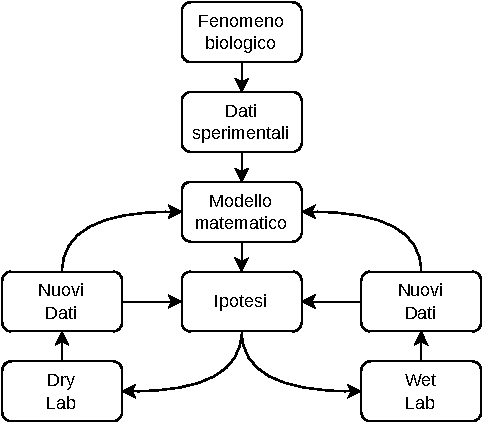
\includegraphics[scale = 0.8]{img/csb.pdf}
  \caption{Grafico rappresentante il processo ciclico della Systems Biology.} 
  \label{fig:csb}
\end{figure}
Un altro aspetto fondamentale del discorso è capire cosa \textbf{non} sia la
\textit{systems biology}. Citando Wolkenhauer \footnote{O. Wolkenhauer, Why
  Systems Biology is (not) called Systems Biology, BIOforum Europe 4/2007}:
\begin{center}
  \textit{Opening then the book, which I discovered in the London bookstore, I
    read the contents list: “Shotgun Fragment Assembly”, “Gene Finding”, “Local
    Sequence Similarities”, ... What?? ... “Protein Structure Prediction”, “Some 
    Computational Problems Associated with Horizontal Gene Transfer” ... what on
    earth has this to do with systems biology, I asked myself?}\\
  \textit{...}\\
  \textit{Most important to me is
    however that cells and proteins are in  teracting in space and time, that
    is, we are dealing here with (nonlinear) dynamic systems. If you ask me
    then, systems biology is a merger of systems theory with cell biology.}
  \\
  \textit{...}\\
  \textit{Systems biology and bioinformatics are different but complementary.}
\end{center}
Infatti tematiche come l'assemblaggio, l'allineamento etc$\ldots$ non sono
tematiche della \textit{systems biolog}y ma della \textit{bioinformatica},
nonostante spesso vengano confuse e sovrapposte. L'analisi diretta dei dati
biologici non è campo della \textit{systems biology} in quanto si perde uno
degli aspetti fondamentali, ovvero quello del \textbf{tempo}, che comporta lo
studio di \textbf{sistemi dinamici}, che appunto di evolvono nel tempo. In
bioinformatica d'altro canto si ha spesso a che fare con dati provenienti da
pochi timestamp (se non direttamente da uno solo). Inoltre, sempre in
bioinformatica, si studiano solitamente poche componenti biologiche, senza
studiarne l'interazione tra esse.\\
La domanda più importante della \textit{systems biology}, della quale possiamo
vedere uno schema generale delle fasi in figura \ref{fig:csb2}, è quindi:
\begin{center}
  \textit{dato un sistema biologico d'interesse, di cui si vogliono studiare le
    funzioni etc$\ldots$, quale approccio modellistico è più adatto per
    descrivere quel sistema?}
\end{center}
Una volta risposto a questo quesito bisogna ovviamente capire quale sia lo
strumento computazionale di cui si ha bisogno per simulare e analizzare tale
sistema. Bisogna infine capire quali predizioni si possono ottenere da questo
modello, che comunque deve prima essere validato. Tra le cose principali che si
vogliono capire abbiamo, ad esempio, se si può controllare il sistema e se si
può riprodurre il tutto in laboratorio riducendo il numero di tentativi e di
conseguenza anche il costo dell'esperimento in \textit{wet lab}.\\
\begin{figure}
  \centering
  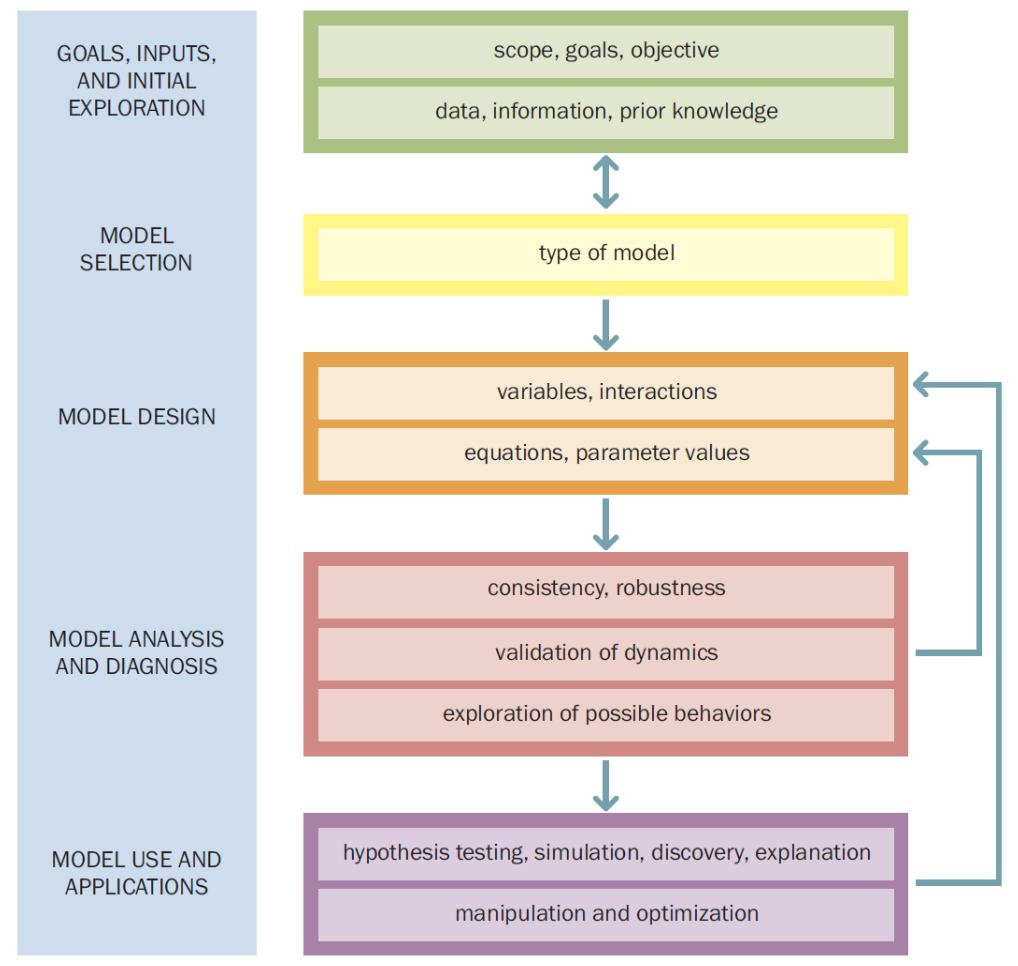
\includegraphics[scale = 0.3]{img/csb2.jpg}
  \caption{Schema generale delle fasi tipiche che compongono la systems
    biology.} 
  \label{fig:csb2}
\end{figure}
Possiamo quindi facilmente intuire che uno degli aspetti fondamentali di questo
ambito è quello di fare le corrette \textit{assunzioni}. Citando ancora
Wolkenhauer \footnote{O. Wolkenhauer, Why Systems Biology is (not) called
  Systems Biology, BIOforum Europe 4/2007}:
\begin{center}
  \textit{The modelling process itself is more important than the model. The
    discussion between the experimentalists and the theoretician, ro decide
    which variables to measure and why, how to formally represent interaction in
    a mathematical form is the basis for succesful interdisciplinary research in
    Systems Biology. In light of the complexity of moleculr systems and the
    available experimental data, Systems Biology is the art of making the right
    assumptions in modelling.}
\end{center}
si nota come il raggiungimento delle assunzioni stesse per ottenere il modello
sia una fase di importanza maggiore rispetto al modello stesso. Il modello
infatti rappresenta la realtà ma non è la realtà stessa e partire da assunzioni
false ed errate porterà ad un modello magari funzionante ``dal punto di vista
sintattico'' ma non `` dal punto di vista semantico'', avendo che esso non potrà
mai essere validato. Nella citazione si parla inoltre di \textit{variabili},
come elemento base dei vari modelli. Tra tali variabili si cercano relazioni,
correlazioni etc$\ldots$\\
Normalmente il punto di partenza sono i \textit{dati omici}.
\begin{shaded}
  Quanto qui riportato è tratto da wikipedia
  \footnote{\url{https://it.wikipedia.org/wiki/-omica}} 
  \begin{definizione}
    In biologia molecolare, ci si riferisce comunemente al neologismo omica (in
    inglese omics) per indicare l'ampio numero di discipline biomolecolari che
    presentano il suffisso ``-omica'', come avviene per la genomica o la
    proteomica. Il suffisso correlato -oma (in inglese -omes) indica invece
    l'oggetto di studio di queste discipline (genoma, proteoma).  
  \end{definizione}
  I più importanti ``-oma'' proposti recentemente all'interno della comunità
  scientifica sono:
  \begin{itemize}
    \item il \textbf{trascrittoma} è l'insieme degli mRNA trascritti nell'intero
    organismo, tessuto, cellula; è studiato dalla trascrittomica
    \item il \textbf{metabolom}a comprende la totalità dei metaboliti presenti
    in un organismo; è studiato dalla metabolomica 
    \item il \textbf{metalloma} comprende la totalità delle specie di metalli e
    metalloidi; è studiato dalla metallomica 
    \item il \textbf{lipidoma} comprende la totalità dei lipidi; è studiato dalla
    lipidomica 
    \item l'\textbf{interattoma} comprende la totalità delle interazioni
    molecolari che hanno luogo in un organismo; un nome che comunemente indica
    la disciplina 
    della interattomica è quello di biologia dei sistemi (systems biology)
    \item lo \textbf{spliceoma} (da non confondersi con lo spliceosoma, il
    complesso di 
    proteine ed acidi nucleici coinvolti nello splicing) comprende la totalità
    delle isoforme proteiche dovute a splicing alternativo; è studiato dalla
    spliceomica
    \item l'\textbf{ORFeoma} comprende la totalità delle sequenze di DNA che
    iniziano con 
    un codone ATG e terminano con un codone di stop (sequenze note come ORF,
    open reading frames). Queste sequenze sono ritenute in grado di codificare
    per una proteina o per una parte
    \item \textbf{textoma}: l'insieme della letteratura scientifica disponibile
    alla consultazione (studiato dalla textomica)
    \item \textbf{kinoma}: l'insieme delle protein chinasi (dall'inglese kinase)
    di una cellula. Esistono pubblicazioni scientifiche che citano il termine
    kinomica 
    \item \textbf{glicosiloma}: correlato alle reazioni di glicosilazione
    (studiato dalla glicosilomica)
    \item \textbf{fisioma}: correlato alla fisiologia (studiato dalla fisiomica)
    \item \textbf{neuroma}: l'insieme delle componenti nervose di un organismo
    (studiato dalla neuromica) 
    \item \textbf{predittoma}: l'insieme delle predizioni di struttura proteica
    \item \textbf{reattoma}: l'insieme dei processi biologici
    \item \textbf{ionoma}: insieme dei nutrienti minerali e degli elementi in
    tracce che si trovano in un organismo 
    \item \textbf{connettoma}: l'insieme di tutti i neuroni e le sinapsi di un
    cervello 
  \end{itemize}
\end{shaded}
Si hanno quindi vari ``livelli'' di studio, al variare dei dati omici, per i
quali variano gli strumenti. Ad esempio:
\begin{itemize}
  \item si ha il \textbf{genoma}, studiato tramite il \textit{sequenziamento},
  la \textit{genotipizzazione} etc$\ldots$
  \item il \textbf{trascrittoma}, ottenuto dopo la \textit{trascrizione},
  studiato tramite \textit{microarrays}, \textit{oligonucleotide chips}
  etc$\ldots$
  \item il \textbf{proteoma}, ottenuto dopo la \textit{traduzione}, studiato
  tramite \textit{proteomica MS-based}, \textit{elettroforesi} etc$\ldots$
  \item il \textbf{metaboloma}, ottenuto tramite le \textit{reazioni}, studiato
  tramite \textit{spettroscopia di massa}, \textit{risonanze magnetiche}
  etc$\ldots$
  \item l'\textbf{interattoma}, ottenuto tramite appunto le varie
  \textit{interazioni}, studiato tramite \textit{screens yeast-to-hybrid}
  etc$\ldots$ 
  \item il \textbf{fenomeno}, ottenuto dopo l'\textit{integrazione} delle varie
  interazioni, studiato tramite \textit{gene inactivations} etc$\ldots$
\end{itemize}
Ognuno di questi ``livelli'' ha una panoramica diversa su quello che sta
accadendo, è accaduto, potrebbe accadere o accadrà ad una certa
cellula. Partendo dalle informazioni dinamiche/cinetiche, ovvero dai dati, e
dalle informazioni strutturali dei vari \textit{pathway} si riesce ad ottenere
la rappresentazione matematica. Ovviamente è impensabile pensare di studiare
tutti i ``livelli'' contemporaneamente ma si può studiare solo una parte del
sistema, studiandone un paio di ``livelli'' o poco più. Inoltre ogni ``livello''
ha associato un suo formalismo matematico, legato alla singola modellazione
matematica. Non sempre tali formalismi sono facilmente integrabili (magari in un
caso ho delle EDO e in un altro dei grafi). Si ha quindi non solo un discorso di
\textit{data integration} ma anche di integrazione dei modelli matematici stessi
e questo non sempre è possibile.\\
Nella realtà, inoltre, prima di scegliere un modello bisogna scegliere
l'\textit{approccio} con cui ottenerlo. Generalmente se ne hanno due in
\textit{systems biology}: 
\begin{enumerate}
  \item l'approccio \textbf{top-down}. In questo caso si parte dalle analisi
  omiche, solitamente con pochissimi timestamp, i cui risultati vengono trattati
  con tecniche bioinformatiche, che riducono anche l'influenza degli errori, per 
  ottenere una \textbf{mappa globale di interazioni}, con le interazioni tra
  migliaia di componenti cellulari, dalla quale si ottiene il
  \textbf{modello predittivo del sistema}. Questo approccio è quindi supportato
  da una grande quantitù di dati basati su \textit{high-throughput} e
  \textit{global profiling}
  \item l'approccio \textbf{bottom-up}. In questo caso si parte dalle
  informazioni, prevalentemente di letteratura, le interazioni tra le componenti
  individuali del sistema, ceracondo magari le concentrazioni o il
  \textit{kinetic-rate}, ovvero a variazione della concentrazione di un reagente
  o di un prodotto nel tempo misurata in moli per secondo
  $\left[\frac{M}{s}\right]$. Tali informazioni potrebbero non essere
  precise. Da  
  queste si formalizza un modello matematico per 
  avere poi comparazioni tra esperimenti e modelli di simulazione, ottenendo
  alla fine il \textbf{modello predittivo del sistema}. Questo approccio soffre
  quindi la mancanza di dati, specialmente di dati quantitativi. Questo
  approccio è più vicino a quello tipico della biologia, avvicinandosi per
  alcuni aspetti al \textit{pensiero riduzionista} (che mira a studiare piccole
  componenti del sistema).\\
  Tale approccio è sicuramente più complesso, per quanto si possa limitare a
  studiare pathway e non l'intero metaboloma, ma per questo anche più
  informativo. 
\end{enumerate}
Ovviamente tali approcci, per quanto sarebbe fantastico, non possono essere
usati in contemporanea. Detto questo solitamente l'approccio top-down studia i
sistemi su larga scala per poi, a volte, procedere con uno studio bottom-up. In
generale comunque la scelta dipende dalla singola situazione. Non esiste un
meglio o un peggio, anche se i modelli generati dall'approccio top-down hanno
generalmente una minor capacità predittiva anche se studiano sistemi più ampi
rispetto all'approccio bottom-up.\\
Bisogna distinguere quindi quali siano le tecniche tipiche della bioinformatica
(ma anche della statistica)
e quali quelle della \textit{systems biology}. L'uso di tecniche per la ricerca
di similarità, correlazioni, causalità probabilistica, clustering (dove si noti
che non ha un ruolo significativo il \textbf{tempo}) etc$\ldots$
non sono di interesse della \textit{systems biology}, che invece è interessata
allo studio delle causalità in cui il \textit{tempo} è intrinseco e
necessario. Questa necessità di avere il \textit{tempo} comporta una maggior
difficoltà nel recuperare i dati e dell'eseguire la sperimentazione ma comporta,
del resto, un forte ``potere di spiegazione e predizione'' da parte del modello
stesso. \\
Vediamo ora qualche definizione di base.
\begin{definizione}
  Definiamo \textbf{modello} come una descrizione rigorosa e assolutamente non
  ambigua di un sistema. Nel dettaglio tale descrizione è ottenuta tramite un
  adeguato formalismo matematico (l'unico per definizione non ambiguo) e un
  adeguato livello di astrazione (importante per non avere informazioni
  ridondanti o inutili nel modello). 
\end{definizione}
\begin{definizione}
  Definiamo \textbf{proprietà/comportamento emergente} ogni
  caratteristica strutturale (quindi di topologia) o dinamica (quindi in
  evoluzione nel tempo) di un sistema che non può essere capita e/o spiegata
  banalmente tramite l'enumerazione delle componenti ma che deve essere derivata
  unicamente come conseguenza tra le componenti stesse del sistema.
\end{definizione}
\begin{definizione}
  Definiamo \textbf{simulazione} come una tecnica ``computer-based'' per
  determinare una qualsiasi caratteristica emergente e/o predire l'evoluzione
  temporale del sistema. 
\end{definizione}
\begin{definizione}
  Definiamo \textbf{metodo computazionale} come una soluzione automatica, basata
  su uno specifico algoritmo, usata per risolvere problemi difficili (da
  intendersi ``difficili'' anche a livello computazionale) e per
  analizzare sistemi in diverse condizioni.
\end{definizione}
Si noti che, come evidenziato da Fawcett e Higginson\footnote{Tim W. Fawcett
  and Andrew D. Higginson, Heavy use of equations impedes communication among
  biologists, PNAS 2012}, l'uso eccessivo dei formalismi matematici rendono
difficile la comunicazione con i biologi, quindi bisogna muoversi di
conseguenza. I modellatori dovrebbero essere preparati a sviluppare nuovi
strumenti matematici e computazionali, invece di ``forzare'' la descrizione e
l'analisi del sistema con un framework preferito e facilmente applicabile (tipo
usare le EDO per tutto a priori). U biologi sperimentali dovrebbero essere aperti
a progettare nuovi protocolli di laboratorio per identificare tutte le
caratteristiche qualitative e, soprattutto, quantitative che ancora mancano (per
aiutare anche i modellisti). \textbf{La parte più interessante del gioco del
  modellismo non è ciò che il modello permette di capire, ma esattamente ciò che
  non è in grado di spiegare}, infatti, secondo, Box:
\begin{center}
  \textit{essentially, all models are wrong, but some are useful.}
\end{center}
e, secondo Bower e Bolouri:
\begin{center}
  \textit{In fact, all modelers should be prepared to answer the question:
    ``what do you know that you did not know before?'' If the answer is ``that i
    was correct'', it is best to look elsewhere.}
\end{center}
Infatti un modello non solo deve rispondere a quello che già si sa ma deve
predire qualcosa che ancora non si sa (magari anche non funzionando).
\section{PCNA ubiquitylation}
Vediamo brevemente uno studio in cui ha partecipato anche la professoressa
Besozzi dove il non funzionamento del modello ha portato ad una nuova scoperta
scientifica \footnote{
  Flavio Amara, Riccardo Colombo, Paolo Cazzaniga, Dario Pescini, Attila
  Csikász-Nagy, Marco Muzi Falconi, Daniela Besozzi, Paolo Plevani , In vivo and
  in silico analysis of PCNA ubiquitylation in the activation of the 
  Post Replication Repair pathway in S. cerevisiae, BMC 2013 }.\\
In questo studio si cercava di studiare la \textbf{Post Replication Repair
  (\textit{PRR})}, ovvero il principale pathway di tolleranza al danno del DNA
che bypassa le lesioni del DNA durante la \textit{fase S}, che è in citologia
(la branca della biologia che studia la cellula dal punto di vista morfologico e
funzionale) una fase del ciclo cellulare, durante la quale il processo
principale è la sintesi e duplicazione del materiale genetico contenuto nel
DNA. Bombardando il lievito con raggi UV si è quindi studiata la proteina
\textbf{PCNA}, ovvero l'\textit{l'antigene nucleare di proliferazione
  cellulare}. La struttura di tale proteina (di forma a ciambella) è in grado di
assumere una peculiare conformazione la quale le consente di contattare il DNA
(DNA clamp) e di promuovere l'azione della polimerasi durante la replicazione
del DNA \footnote{\url{https://it.wikipedia.org/wiki/PCNA}}. I raggi UV
provocano lesioni che vengono ``trattate'' dalla PCNA. Se ne è quindi
studiata l'\textbf{ubiquitazione}, modificazione post-traduzionale di una
proteina dovuta al legame covalente di uno o più monomeri di ubiquitina. Tale
legame porta, solitamente, alla degradazione della proteina
stessa\footnote{\url{https://it.wikipedia.org/wiki/Ubiquitina}}. La
\textit{mono-ubiquitazione} avviene tramite gli enzimi \textit{Rad6}
\textit{Rad8} mentre la \textit{poli-ubiquitazione} tramite gli enzimi
\textit{Rad5} e \textit{Ubc13-Mms2}. La prima comporta errori di trascrizione,
in quanto si aveva sintesi di DNA tra le lesioni, formando \textit{mutageni},
mentre la seconda è ``error free''.\\
Si conoscevano quindi i principali attori del fenomeno, ovvero la proteina e gli
enzimi. C'erano varie cose che però non si conoscevano:
\begin{itemize}
  \item l'ordine spazio temporale della cascata delle interazioni delle varie
  proteine, non sapendo anche i tempi di attivazione dei vari enzimi
  \item se il numero di lesioni influenzasse il bilanciamento tra le
  \textit{mono-ubiquitazioni} e le \textit{poli-ubiquitazioni}
  \item se esistesse una soglia relativa al danno che regolasse l'interazione
  tra i due sub-pathway
\end{itemize}
Si è quindi proceduto, in \textit{wet lab}, irradiando il lievito in modo
controllato, misurando \textit{mono-ubiquitazioni} e le
\textit{poli-ubiquitazioni} al passare del tempo (da 0 a 300 minuti) a varie
dosi di UV, e contemporaneamente studiando un modello matematico (tramite le
varie reazioni, rappresentate tramite \textit{prodotti} e \textit{reagenti}) per
effettuare le simulazioni. Si è visto, in laboratorio, che 
le varie forme ubiquitilate di PCNA sono assenti a basse dosi di UV
($5\frac{J}{m^2}$ e $10\frac{J}{m^2}$), mentre ad alte dosi di UV
($50\frac{J}{m^2}$ e $75\frac{J}{m^2}$) entrambi i segnali sono ancora presenti
dopo 5 ore nei \textit{western blot}. La simulazione matematica confermava
quanto stesse succedendo a 
bassi dosaggi ma non riusciva ad ottenere i risultati ad alti dosaggi. Dopo vari
tentativi, rifacendo gli esperimenti (variando enzimi e geni) e sistemando il
modello (tramite \textit{parameter sweeping/estimation, analisi di sensitività})
si è sospettato che il modello fosse in realtà ``corretto'' ma non 
completo, mancava qualche ipotesi. Da qui la scoperta: si ha anche un altro
pathway, il \textbf{Nucleotide Excision Repair (\textit{NER})} che ``assiste''
la \textit{PCNA} quando le cellule sono gravemente lesionate. NER è infatti
attivo nella \textit{fase S} e serve alla \textit{PRR} per funzionare
correttamente \textit{in vivo}. Risistemando il modello con \textit{NER} ed
enzimi annessi le simulazioni hanno funzionato. \\
Questa è la prova che quando un modello non funziona si può ottenere anche una
scoperta scientifica, ed è una delle situazioni (coi giusti limiti) più
interessanti di questa branca di ricerca.
\section{I Sistemi Complessi}
In \textit{systems biology} si ha quindi a che fare con sistemi che vengono
definiti \textbf{sistemi complessi}, ovviamente presi nella loro ``sottoclasse''
relativa ai sistemi biologici.
\begin{definizione}
  Si definisce un \textbf{sistema complesso} con un sistema consistente di un
  certo numero di componenti più o meno semplici che, prese nel loro insieme,
  danno vita ad un \textit{comportamento emergente}, grazie alle loro
  \textit{mutue interazioni}. 
\end{definizione}
In questo contesto assumono importanza tre concetti chiave:
\begin{enumerate}
  \item \textbf{comportamento non lineare}, quindi non facilmente prevedibile
  \item \textbf{sistema aperto}, ovvero dove l'interazione con l'ambiente da
  parete del sistema è una delle caratteristiche da studiare e modellare
  \item \textbf{sistema dinamico}, ovvero si ha che il sistema evolve nel tempo 
\end{enumerate}
Uno dei punti cruciali è inoltre capire che quando si procede alla modellazione
di un certo sistema non si deve modellare anche cosa ci si aspetta da quel
modello. Tale informazione infatti deve scaturire dalle simulazioni del modello
stesso in modo completamente autonomo.\\
Come visto si studiano quindi insiemi di componenti. L'insieme complessivo delle
funzionalità del sistema non è determinato però da una specifica funzione di
ogni componente ma dalle loro interazioni. Si hanno quindi altri due concetti
chiave:
\begin{enumerate}
  \item \textbf{topologia/architettura interna}
  \item \textbf{moduli funzionali}
\end{enumerate}
Anche componenti molto semplici possono dare vita a un sistema complesso.\\ 
Vediamo quindi qualche esempio di sistema complesso:
\begin{itemize}
  \item un esempio ``semplice'' è quello di una \textbf{reazione enzimatica con
    feedback negativo}. In questo caso si hanno una serie di \textit{reazioni
    lineari} che dal legame di un \textit{substrato} portano ad un
  \textit{prodotto}. La complessità viene data dal \textit{feedback negativo} in
  quanto la produzione del prodotto stesso porta il substrato a non  legare. Si
  ha quindi la cosiddetta \textbf{autoregolazione} che rende questo un vero e
  proprio \textit{sistema complesso}, avendo che il comportamento emergente del
  sistema è in realtà difficile da prevedere.\\
  Ovviamente si potrebbe anche assumere il caso meno semplice dove si ha una
  serie di \textit{reazioni non lineare}. \\
  Si può quindi arrivare anche a parlare di casi più ``estesi'', come quello ad
  esempio di un \textbf{pathway metabolico}. Ci sarebbe inoltre un caso,
  seguendo questo filo pensiero, ancora più estremo, ovvero quello del
  \textbf{metabolismo di un'intera cellula}, come visualizzabile nella figura
  \ref{fig:meta}, dove si hanno moltissime parti che 
  nel dettaglio sono lineari ma che si autoregolano a vicenda, ottenendo quindi
  un \textit{sistema complesso} davvero impossibile da studiare.
  \begin{figure}
    \centering
    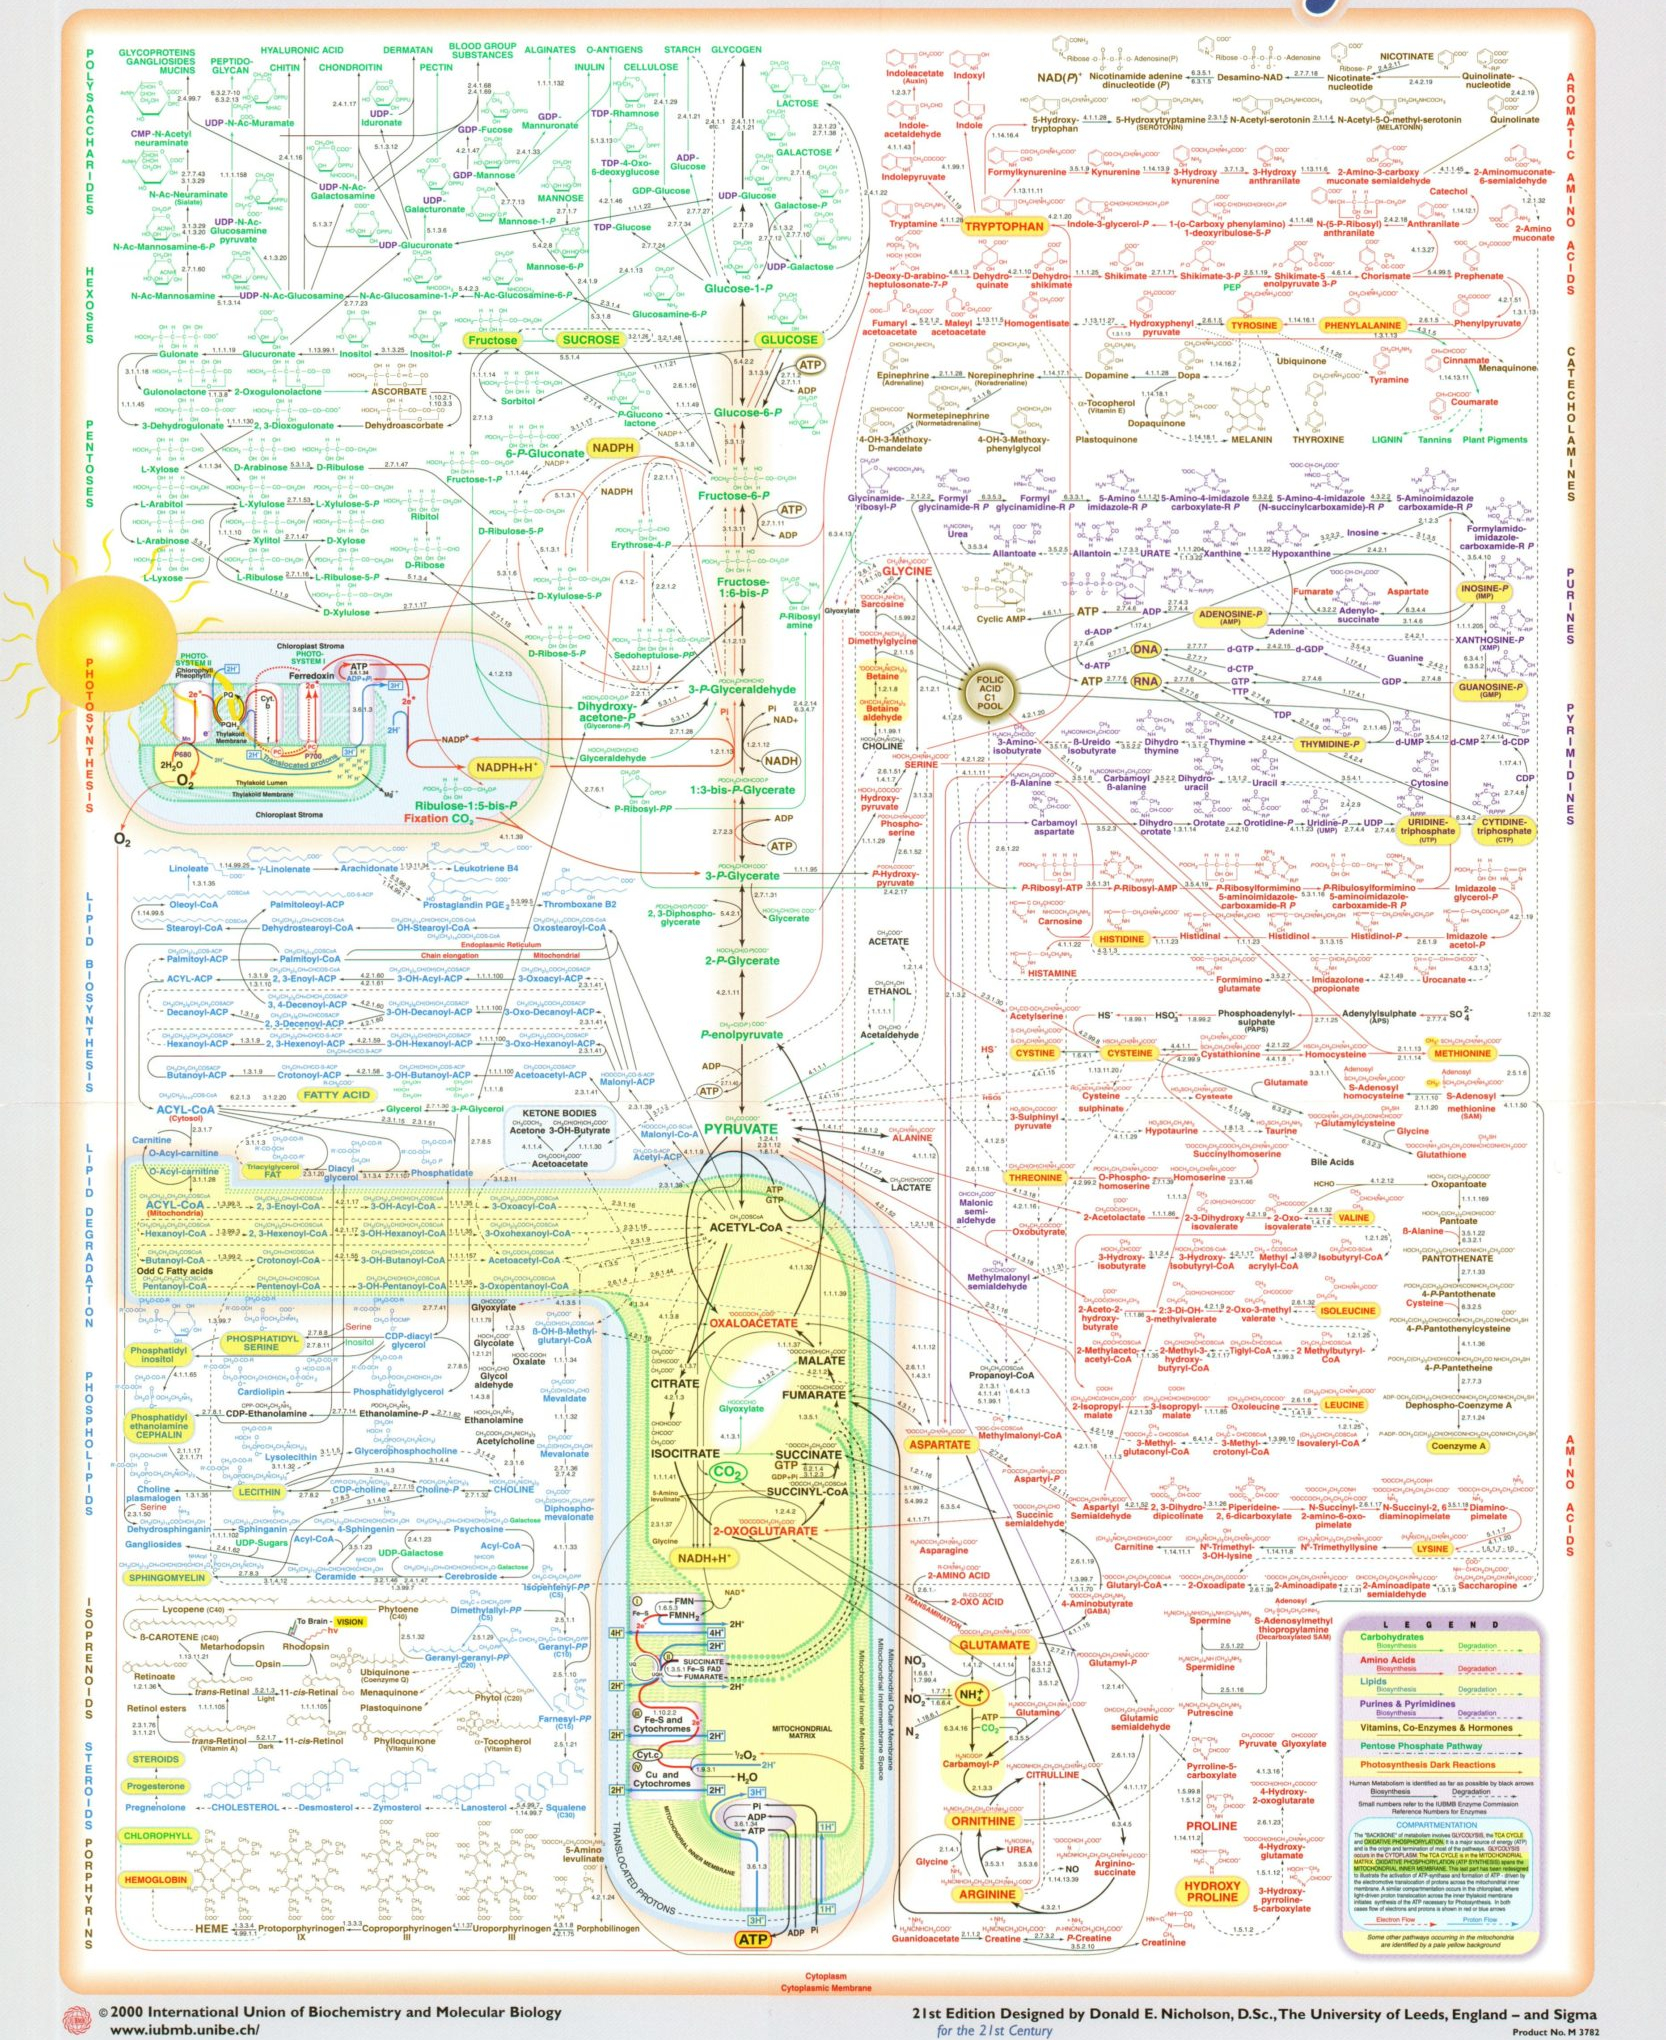
\includegraphics[width = \textwidth]{img/metabolome.jpg}
    \caption{Insieme dei pathway che ``compongono'' il metabolismo di un'intera
      cellula. Tale rappresentazione è stata fatta da Donald E. Nelson,
      dell'università di Leeds e dall'azienda Sigma-Aldrich per la International
      Union of Biochemistry and Molecular Biology del 2000.}
    \label{fig:meta}
  \end{figure}
  \item un altro esempio può essere quello di una \textbf{rete di interazioni
    proteina-proteina (\textit{protein-protein interaction network})} dove si
  hanno:  
  \begin{itemize}
    \item \textbf{nodi} che rappresentano le proteine
    \item \textbf{archi} che rappresentano \textbf{interazioni fisiche} e
    \textbf{interazioni funzionali} tra proteine (???)
  \end{itemize}
  In questo caso la ``complessità'' è data soprattutto dal numero
  incredibilmente alto di proteine (quindi di nodi) e di interazioni tra esse
  (quindi di archi) nel nostro sistema. Un esempio è visualizzabile in figura
  \ref{fig:ppn}. 
  \begin{figure}
    \centering
     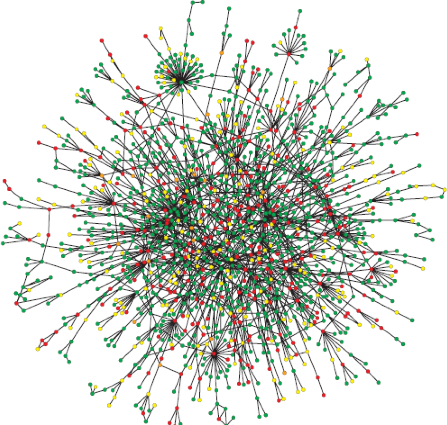
\includegraphics[width = \textwidth]{img/ppn.png}
    \caption{Esempio di rete di interazioni
      proteina-proteina,
      \url{https://www.ebi.ac.uk/training/online/courses/network-analysis-of-protein-interaction-data-an-introduction/protein-protein-interaction-networks/}. In
    tale rete si ha lo studio sul lievito e i vari colori dei nodi rappresentano
    vari effetti fenotipici legati alla rimozione della proteina rappresentata
    dal nodo stesso. Si ha rosso per l'effetto letale, verde per l'effetto non
    letale, arancione per la crescita lenta e giallo per effetto sconosciuto.}
     \label{fig:ppn}
  \end{figure}
  \item un altro esempio è quello delle \textbf{reti di regolazione genica
    (\textit{gene regulatory network})} dove appunto si studiano le relazioni
  che si hanno tra le espressioni e le regolazioni tra geni. In questo caso si
  hanno: 
  \begin{itemize}
    \item \textbf{nodi} che rappresentano i geni
    \item \textbf{archi} che rappresentano le regolazioni tra geni
  \end{itemize}
  Anche in questo caso si possono avere feedback e tali reti sono utili per
  studiare l'\textit{over-espressione di geni}. Inoltre deve essere chiaro che
  la modifica in un certo gene si ripercuote, chi più chi meno, sull'intera
  rete anche se non si ha un singolo gene che ``controlla'' l'intera rete ma
  tutti contribuiscono alla funzionalità dell'intero sistema complesso
  \item aumentando ancora il livello di complessità potremmo pensare allo studio
  di un certo pathway, come ad esempio il \textit{segnale di trasduzione}, in
  una cellula tenendo però conto anche della \textit{componente spaziale},
  tridimensionale, della stessa,  
  nonché le interazioni con l'ambiente. La componente spaziale, che ovviamente
  aggiunge complessità, è una parte rilevante del modello, come il ``movimento''
  al suo interno (prestando sempre attenzione a non aggiungere componenti
  inutili al modello stesso). L'interazione con l'ambiente può portare, ad
  esempio, a \textit{cascate di reazioni intra-cellulari} e a vari ``input'',
  come \textit{ormoni, fattori di sopravvivenza, fattori di
    crescita/anti-crescita, fattori di morte etc$\ldots$} da considerare nel
  modello 
  \item un altro esempio ancor più ``complesso'' può essere quello della
  \textbf{crescita tumorale}, magari ponendo al centro dello studio anche il
  rapporto tra essa e la \textbf{vascolarizzazione}, ovvero la distribuzione di
  vasi sanguigni in un tessuto, in quanto magari si vuole studiare la vicinanza
  tra il tumore e i vasi sanguigni. In questo contesto non solo lo spazio
  tridimensionale è di fondamentale importanza ma bisogna anche modellare
  cellule di vario tipo (normali, cancerogene, legate al sistema immunitario, in
  apoptosi, necrotiche
  etc$\ldots$), che interagiscono in modo diverso tra loro, magari avendo anche
  ``mutazioni'' da normali a cancerogene etc$\ldots$ Si hanno quindi componenti
  eterogenee, dovendo per lo più anche modellare i vasi sanguigni e le
  interazioni con le cellule.
  \item un altro esempio, ``complesso'' almeno quanto il precedente, è lo studio
  della \textbf{formazione di biofilm}, ovvero una aggregazione complessa di
  microrganismi contraddistinta dalla secrezione di una matrice adesiva e
  protettiva. Tale barriera è comunque una struttura permeabile permettendo il
  passaggio dei nutrienti. In un biofilm i microrganismi, tendenzialmente batteri, non solo
  crescono ma, soprattutto quelli più interni e ``protetti'', diventano anche
  più resistenti. Questa è una seria complicazione per la loro eliminazione
  quando fuoriescono dal biofilm. Anche qui quindi bisogna modellare lo spazio
  tridimensionale, l'interazione con l'ambiente, l'interazione tra i vari
  microrganismi (anche se si ha solitamente poca eterogeneità)
  \item cambiando prospettiva un altro esempio di \textit{sistema complesso} è
  quello dello \textbf{sviluppo embrionale e della differenziazione cellulare}
  dove, a partire dall'embrione e da cellule staminali si vanno a formare tutti
  i tipi di cellule che formeranno, ad esempio, i tessuti, gli organi
  etc$\ldots$ dell'uomo. In questo caso solitamente si ha un tipo di
  modellazione diverso, basato su componenti semplici 
  \item un altro esempio è quello dello studio dell'\textbf{ecosistema}. Nel
  dettaglio uno degli aspetti studiati è quello della cosiddetta
  \textbf{dinamica preda-predatore}. Tale dinamica descrive il rapporto tra il
  numero di prede e di predatori e osserva un comportamento oscillatorio (se
  aumentano i predatori diminuiscono le prede fino a che non sono abbastanza per
  i predatori, che calano di numero, portando il numero di prede a crescere
  etc$\ldots$) 
  \item infine un ultimo esempio, molto attuale, di \textit{sistema complesso} è
  quello dello \textbf{studio epidemiologico della diffusione di
    epidemie/pandemie} dove la ``complessità'' è incrementata anche dagli
  aspetti sociali e psicologici delle persone, nonché dalla loro eterogeneità
  anche nel dominio epidemiologico (infetti, gravemente infetti, guariti,
  esposti, suscettibili all'infezione, morti etc$\ldots$)
\end{itemize}
In questi esempi si è spesso parlato più o meno esplicitamente di
\textbf{livelli di complessità}. Per poter avere un'idea di quanti possano
essere bisogna considerare vari punti di vista:
\begin{itemize}
  \item un primo punto di vista è dato dalla \textbf{scala spaziale} dei
  fenomeni che si studiano. Possiamo studiare infatti eventi che accadono nel
  range dei nanometri, o meno, fino a pensare ad eventi in scala umana, in
  metri. Inoltre 
  anche un evento che avviene in nanometri può avere conseguenze visibili in
  metri. Questo tipo di complessità è per lo più un problema matematico dal
  punto di vista della gestione della stessa
  \item un secondo punto di vista è dato dalla \textbf{scala temporale} dei
  fenomeni che si studiano. Anche in questo caso si passa dai nanosecondi, o
  meno, ai miliardi di anni. Un evento quasi istantaneo può avere conseguenze
  evolutive tra milioni di anni. La gestione di questo tipo di complessità è un
  grande problema dal punto di vista computazionale. La complessità aumenta
  all'aumentare della scala temporale
  \item altri livelli di complessità sono dati dai \textit{livelli di funzione
    di un organismo}, avendo, ad esempio, che da \textit{trascrittoma, proteoma}
  e \textit{metaboloma}, in ottica pathway, si passa al \textit{fisioma}, in
  ottica cellule, tessuti, organi e direttamente l'uomo
\end{itemize}
Pensando anche solo alla scala spaziale e quella temporale si ha inoltre che
esse sono in sinergia ma è comunque pressoché impossibile pensare ad un modello
che tenga traccia in modo completo o quasi di entrambe queste scale.
\section{Rappresentazione Grafica}
Ai biologi/biotecnologi etc$\ldots$ piace fare diagrammi e mappe concettuali per
rappresentare graficamente le conoscenze biologiche che hanno su un sistema, ad
esempio componenti molecolari e le loro mutue relazioni, formazione di complessi
molecolari, presenza di feedback di regolazione positivi/negativi
etc$\ldots$. Come si intuisce facilmente diagrammi di questo tipo sono soggetti
ad interpretazioni ambigue e limitano anche l'esplicita rappresentazione della
conoscenza biologica. La matematica è l'unico linguaggio non ambiguo e
fortunatamente esistono anche formalismi, come i \textit{grafi}, le \textit{reti
  di Petri} etc$\ldots$ che non solo sono formalmente rigorosi ma hanno anche
un'interpretazione grafica (tanto amata dalle persone). Ovviamente non sempre si
hanno queste soluzioni intermedie. La modellazione
matematica risolve ogni errata interpretazione e descrive in modo non ambiguo
quello che accade nel sistema e può potenzialmente includere ogni tipo di
ipotesi che può poi essere studiata e testata in \textit{wet lab}. In ogni caso
i diagrammi possono avere utilità nella fase preliminare di discussione tra il
biologo e il modellista: può essere un buon punto di partenza ma non sarà mai
sufficiente per modellare il sistema, che si può ottenere solo con la
formalizzazione matematica di componenti e interazioni. Un esempio è
visualizzabile in figura \ref{fig:dia}\footnote{Besozzi D. (2016) Reaction-Based
  Models of Biochemical Networks. In: Beckmann A., Bienvenu L., Jonoska N. (eds)
  Pursuit of the Universal. CiE 2016. Lecture Notes in Computer Science, vol
  9709. Springer, Cham. https://doi.org/10.1007/978-3-319-40189-8\_3}. 
\begin{figure}
  \centering
  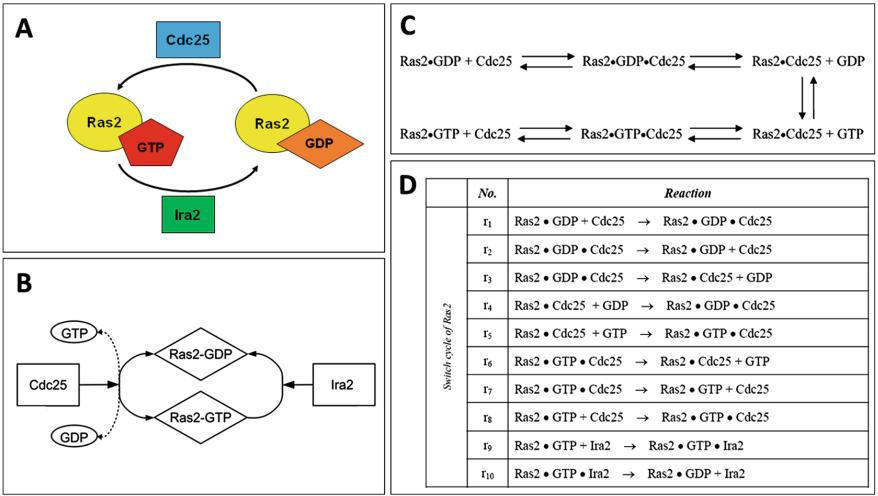
\includegraphics[scale = 0.4]{img/dia.jpg}
  \caption{Esempio (senza entrare nei dettagli biologici che sarebbero ora
    superflui) di un diagramma ambiguo, in figura \textit{A}, tipico 
    dell'approccio biologico. Si hanno poi successive migliorie formali fino ad
    arrivare al modello matematico preciso, in figura \textit{D}, e non ambiguo
    formato da 10 reazioni biochimiche.} 
  \label{fig:dia}
\end{figure}
\section{Tipologie di Modelli}
Sistemi biologici differenti necessitano di approcci modellistici differenti,
ovvero di framework matematici, quindi ad un preciso formalismo, e
conseguentemente computazionali diversi. Inoltre bisogna sempre tenere in
considerazione che ogni metodo computazionale legato ad un preciso modello può
rispondere solo a certe tipologie di domande. Non si ha però una corrispondenza
biunivoca tra ogni approccio modellistico e ogni sistema biologico, infatti
diversi modelli potrebbero prestarsi bene ad un certo sistema biologico (anche
se alcuni modelli sono inapplicabili per certi sistemi biologici o per certe
domande su tali sistemi). La scelta del modello è quindi fortemente legata alle
entità che si vogliono rappresentare e alle risposte che si vogliono ottenere
dal modello. \textbf{Non si ha una strategia universalmente valida per scegliere
il miglior approccio modellistico in base al sistema biologico d'interesse.}\\
Il primo passo è quindi l'interazione tra il biologo/biotecnologo e il
modellista. Il primo deve porsi varie domande tra cui:
\begin{itemize}
  \item cosa si sa e cosa non si sa del sistema biologico in questione?
  \item che tipologie di dato di laboratorio sono disponibili?
  \item che tipologie di dato posso misurare effettivamente i9n laboratorio? 
\end{itemize}
Anche il modellista quindi si deve porre delle domande fondamentali, tra cui:
\begin{itemize}
  \item quale formalismo matematico si presta meglio per questo problema?
  \item che strumenti computazionali sono necessari?
  \item che tipo di predizioni mi aspetto dal modello?
\end{itemize}
Queste questioni sono ``in ciclo'' tra di esse e sono la base degli studi in
\textit{systems biology}, dove farsi domande è una parte fondamentale. In merito
all'ultima domanda del biologo è 
interessante notare che un modello \textbf{deve} essere validato in
laboratorio. Qualora non sia possibile, ad esempio un ``caso limite'' emerso
dallo studio del modello, non si può fare nulla (anche se, qualora
si avessero più modelli completamente distinti che portano allo stesso risultato
si può presupporre che ci sia un fondo di verità). \\
La domanda fondamentale resta però:
\begin{center}
  \textit{qual è la questione scientifica? Perché mi serve un modello?}
\end{center}
La risposta a questa domanda deve essere ``sicura'' prima di intraprendere uno
studio di modellazione.\\
Nel dettaglio, durante il corso, si vedranno i quattro approcci modellistici
tradizionali più usati anche se si tratta di una selezione tra la moltitudine
degli approcci presenti:
\begin{enumerate}
  \item \textbf{modelli basati su interazioni (\textit{interaction-based
      models})}
  \item \textbf{modelli basati su vincoli (\textit{constraint-based
      models})}
  \item \textbf{modelli logici (\textit{logici-based models})}
  \item \textbf{modelli meccanicistici (\textit{mechanism-based models})}
\end{enumerate}
Un generale dato un certo sistema biologico d'interesse, dopo aver risposto alla
domanda fondamentale e avendo quindi ben chiaro il fine di tale modello, la
scelta del modello stesso viene presa considerando secondo quattro aspetti
fondamentali:
\begin{enumerate}
  \item la \textbf{dimensione del sistema}, data in primis dal numero di
  componenti e dal numero delle interazioni tra esse. Si distinguono, secondo
  questo aspetto, due grandi macro-categorie di sistemi:
  \begin{enumerate}
    \item \textbf{sistemi small-scale}, se siamo nel range delle unità o delle
    decine di componenti/interazioni
    \item \textbf{sistemi large-scale}, se siamo nel range delle centinaia o
    migliaia (se non oltre) di componenti/interazioni 
  \end{enumerate}
  Questo è già un ottimo fattore discriminatorio per la scelta del sistema 
  \item il \textbf{livello di dettaglio} necessario a descrivere in modo
  completo le componenti del sistema e le loro interazioni. Si ricorda sempre
  però che formalizzare informazioni inutili e/o ridondanti comporta solo
  un'inutile spreco dal punto di vista computazionale
  \item il \textbf{tipo} e la \textbf{qualità} dei \textbf{dati sperimentali}
  che sono già disponibili o che si è in grado di produrre all'evenienza con
  precisi protocolli al fine di supportare la fase di modellazione. Tali dati
  possono essere ad esempio \textit{dati omici, western blots} etc$\ldots$
  \item il \textbf{carico computazionale} che l'approccio scelto comporta in
  fase di simulazione e analisi dei dati. Un esempio è quello della
  \textit{dinamica molecolare}, che studia come interagiscono tra loro più
  molecole (o anche il comportamento interno di una sola). Tali studi
  normalmente impiegano settimane per simulare anche range temporali molto
  ridotti e necessitano di molte informazioni che non possono essere trascurate
  per ottenere un modello ed una simulazione realistici. Questa scelta è spesso
  un trade-off nella scelta di \textbf{approcci modellistici quantitativi} e
  \textbf{approcci modellistici qualitativi}.\\
  L'uso di \textbf{super computer}, di \textbf{tecniche di calcolo parallelo su
    GPU} etc$\ldots$ sono molto comuni in \textit{systems biology}
\end{enumerate}
Una misura fondamentale è poi la \textbf{capacità predittiva del modello} che,
se bassa, ci porta a preferire \textit{modelli qualitativi}, se alta invece a
\textit{modelli quantitativi}.\\
Si ha quindi un comodo grafico che classifica le quattro tipologie di modelli
in base a questi quattro aspetti\footnote{Besozzi D. (2016) Reaction-Based
  Models of Biochemical Networks. In: Beckmann A., Bienvenu L., Jonoska N. (eds)
  Pursuit of the Universal. CiE 2016. Lecture Notes in Computer Science, vol
  9709. Springer, Cham. https://doi.org/10.1007/978-3-319-40189-8\_3} in figura
\ref{fig:appro}. 
\begin{figure}
  \centering
  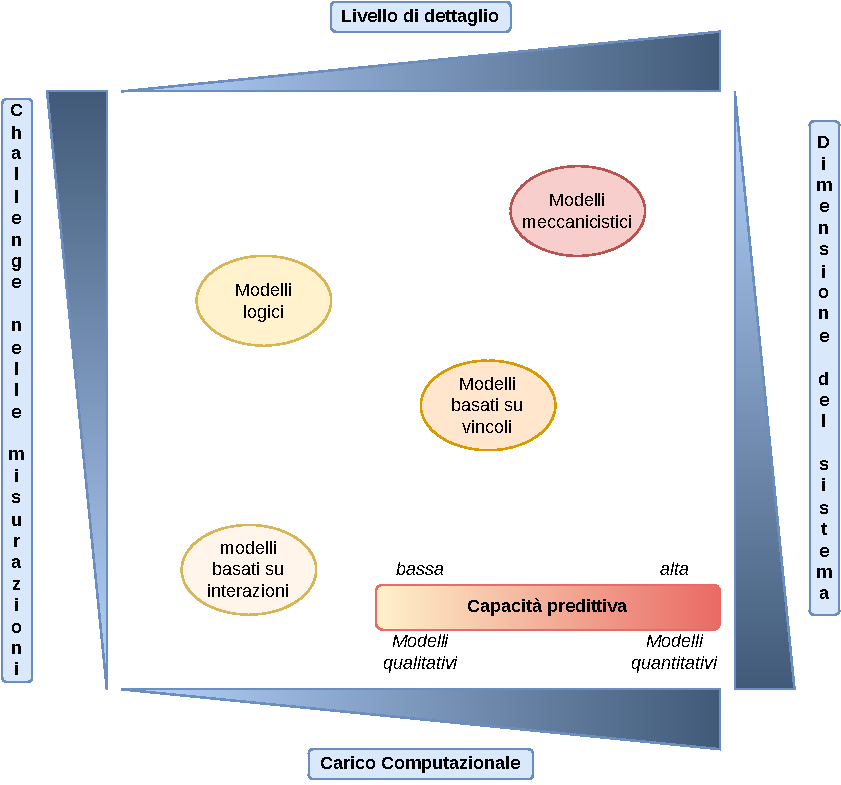
\includegraphics[width = \textwidth]{img/choice.pdf}
  \caption{Schema riassuntivo dei quattro approcci}
  \label{fig:appro}
\end{figure}
Nel grafico notiamo come i \textit{modelli meccanicistici}, tra quelli
analizzati, siano 
quelli con il più alto potere predittivo, che è un aspetto fondamentale ma anche
con i più alti livelli di 
dettaglio, costi computazionali e sfide nella misurazione dei dati
richiesti. L'ovvia conseguenza è che la dimensione del sistema da studiare deve
essere ridotta, avendo quindi \textit{sistemi small-scale}.\\
Si noti che collocare i \textit{modelli logici} non sia così banale in quanto il
livello di dettaglio e la facilità di misurazione possono essere migliorati
usando ad esempio le \textbf{logiche fuzzy}.\\
Un altro aspetto fondamentale da tenere in considerazione è che il processo di
modellazione richiede molto tempo e si basa su continui rifinimenti del modello
stesso, in un processo circolare, come visualizzabile in figura
\ref{fig:cyc}\footnote{Chou IC, Voit EO. Recent developments in parameter
  estimation and structure identification of biochemical and genomic
  systems. Math
  Biosci. 2009;219(2):57-83. doi:10.1016/j.mbs.2009.03.002}. Quindi partendo dai
dati biologici si abbozza un primo modello che viene poi continuamente sistemato
tramite nuove ipotesi, altri dati, analisi \textit{in silico} etc$\ldots$ fino
all'ottenimento di un modello validato.
\begin{figure}
  \centering
  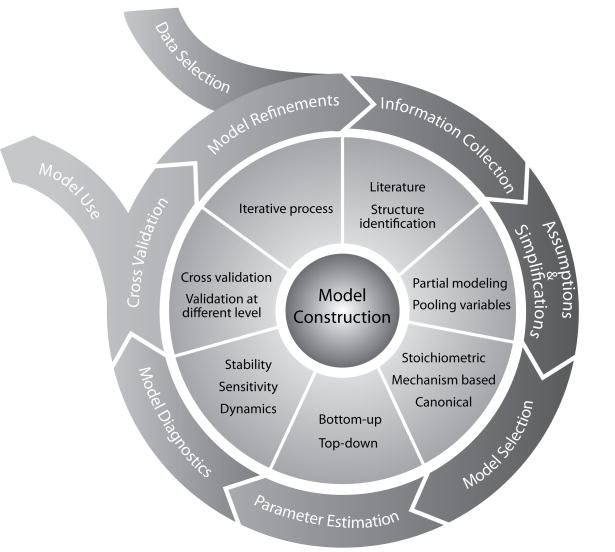
\includegraphics[scale = 0.8]{img/cycle.jpg}
  \caption{Raffigurazione che mostra i dettagli del processo ciclico di
    modellazione in \textit{systems biology}. Molte, ma non tutte, delle keyword
    presenti verranno approfondite nel corso}
  \label{fig:cyc}
\end{figure}
Vediamo ora una breve introduzione ai quattro approcci elencati al fine di poter
fare un confronto tra essi prima di studiarli e formalizzarli nel dettaglio.\\
Prima di fare ciò diamo una più precisa idea dei criteri con cui si classifica
un modello.
\begin{definizione}
  Si definisce \textbf{modello qualitativo} un modello che specifica le
  interazioni tra le componenti del modello stesso.
\end{definizione}
\begin{definizione}
  Si definisce \textbf{modello quantitativo} un modello che assegna un valore ad
  ogni elemento che descrive e anche alle interazioni tra essi. In questo caso
  si possono avere o non avere cambiamenti nel modello.
\end{definizione}
\begin{definizione}
  Si definisce \textbf{modello deterministico} un modello per il quale
  l'evoluzione attraverso i vari stati può essere predetta a partire dallo stato
  corrente, nel dettaglio anche dallo \textit{stato iniziale}. Il comportamento
  evoluzionistico del modello quindi non varierà tra una simulazione e l'altra.
\end{definizione}
\begin{definizione}
  Si definisce \textbf{modello stocastico} un modello che descrive, a partire da
  uno stato corrente, uno stato futuro attraverso una \textit{distribuzione di
    probabilità}.
\end{definizione}
\begin{definizione}
  Un processo è detto \textbf{reversibile/irreversibile} se si può o meno
  procedere in avanti o indietro tra i vari stati.
\end{definizione}
\begin{definizione}
  Con il termine \textbf{periodicità} si intende che il sistema assume una serie
  di stati nell'intervallo di tempo $[t, t+\Delta t]$ ma anche in:
  \[[t+i \Delta t, t+(i+1)\Delta t],\,\,i=1,2,3,\ldots\]
\end{definizione}
\subsection{Modelli Basati su Interazioni}
Questo tipo di modelli vengono usati per \textit{sistemi large-scale} con
centinaia o migliaia di componenti che interagiscono tra loro in modo fisico o
funzionale. Abbiamo vari esempi di questi modelli, tra cui:
\begin{itemize}
  \item \textbf{reti di interazioni proteina-proteina}
  \item \textbf{reti di regolazione genica}
  \item \textbf{reti metaboliche}
  \item \textbf{reti di malattie}, modelli più complessi, modellati tramite un
  particolare tipo di grafo, che sfruttano
  l'integrazione tra \textit{reti di regolazione genica} e grafi/reti
  rappresentanti le malattie e le relazioni tra esse. Si ottiene quindi un grafo
  che mette in relazione componenti genomiche e malattie
\end{itemize}
In questo caso la scelta del formalismo matematico ricade principalmente sulla
\textbf{teoria dei grafi} e si ha quindi un \textit{modello qualitativo} e
\textit{statico}. Infatti il \textit{tempo} non viene considerato in tali
modelli, che di conseguenza non permettono di ottenere informazioni su
eventuali \textbf{comportamenti emergenti}. Non si possono nemmeno ottenere
informazioni quantitative.\\
Parlando di \textit{modelli basati su interazioni} non si può propriamente
parlare di ``simulazioni'' vere e proprie in quanto in primis manca la
modellazione del \textit{tempo} ma anche di altri fattori come il
\textit{kinetic rate}. Inoltre tali modelli difettano anche di una qualsivoglia
modellazione dello \textit{spazio}. Il fulcro dello studio di tali modelli
quindi solitamente si concerta sulle proprietà ``architetturali'' della
struttura della rete, studiando, ad esempio:
\begin{itemize}
  \item la presenza di \textbf{hub}, ovvero nodi in cui sono entranti/uscenti un
  gran numero di archi rispetto agli altri nodi della rete
  \item misure di centralità
  \item presenza di \textit{motivi (motifs)} nella rete
  \item la robustezza topologica
\end{itemize}
Tutte queste misure permettono anche di caratterizzare, caratterizzando la
topologia stessa, una rete rispetto ad un
altra. Infatti si vedranno vari tipologie di rete, tra cui:
\begin{itemize}
  \item \textbf{random network}
  \item \textbf{scale-free network}, caratterizzate da una forte
  \textit{robustezza}
  \item \textbf{hierarchical network}
\end{itemize}
\subsection{Modelli Logici}
Questi modelli possono essere usati sia per sistemi \textit{small-scale} che per
sistemi \textit{large-scale} e alcuni degli esempi sono:
\begin{itemize}
  \item \textbf{reti di regolazione gene-gene}
  \item \textbf{pathway di trasduzione del segnale} (che si ricorda essere la
  capacità di una cellula di convertire uno stimolo esterno in una particolare
  risposta cellulare) 
  \item \textbf{differenziazione cellulare}
  \item \textbf{pathway per la morte cellulare programmata}
\end{itemize}
Il primo caso è un esempio di \textit{sistema large-scale} mentre gli altri di
\textit{sistemi small-scale}.\\
Dal punto di vista del formalismo matematico si ha anche qui la \textbf{teoria
  dei grafi}, a cui viene aggiunta la \textbf{logica booleana}, con i classici
operatori logici $\neg,\land,\lor$, o anche,
preferibilmente, la \textbf{logica fuzzy}, che verrà approfondita più avanti. L'idea di base è quella che lo stato
delle componenti è regolato da altre componenti del sistema stesso. I nodi
possono assumere o valore booleano 0/1 o, in logica fuzzy, qualsiasi valore tra
0 e 1 (con varie conseguenze nel loro studio).\\
Tali modelli sono in grado di simulare il tempo, rientrando quindi nella
categoria dei \textit{sistemi dinamici} ma sono anch'essi della tipologia dei
\textit{modelli qualitativi}. Tali sistemi si prestano ad essere sia
\textit{deterministici} che \textit{non deterministici}.\\
Lo studio di tali modelli solitamente consiste, tramite le simulazioni e le
analisi, nel determinare:
\begin{itemize}
  \item \textbf{cicli}, ovvero sequenze finite di stati complessivi del sistema
  che si ripetono
  \item \textbf{attrattori}, ovvero degli \textit{stati finali} che sono
  raggiungibili da qualsiasi stato iniziale e una volta raggiunti sio resta in
  tali stati
  \item \textbf{bacini di attrattori}, ovvero percorsi che partono da stati
  intermedi e che conducono a degli \textit{attrattori}
\end{itemize}
Tendenzialmente si arriva sempre ad un \textit{ciclo} o ad un insieme di
\textit{attrattori}.\\
La ``potenza'' della \textit{logica fuzzy} permette, come detto, anche di
modellare il \textit{tempo}, derivando quindi un comportamento dinamico del
sistema, descrivendo, ad esempio, la variazione nel tempo tra i valori degli
stati di ogni componente.\\
Un esempio semplice di quello che si può ottenere con tali modelli è
visualizzabile in figura \ref{fig:log}\footnote{Wynn ML, Consul N, Merajver SD,
  Schnell S. Logic-based models in systems biology: a predictive and
  parameter-free network analysis method. Integr Biol
  (Camb). 2012;4(11):1323-1337. doi:10.1039/c2ib20193c}. 
\begin{figure}
  \centering
  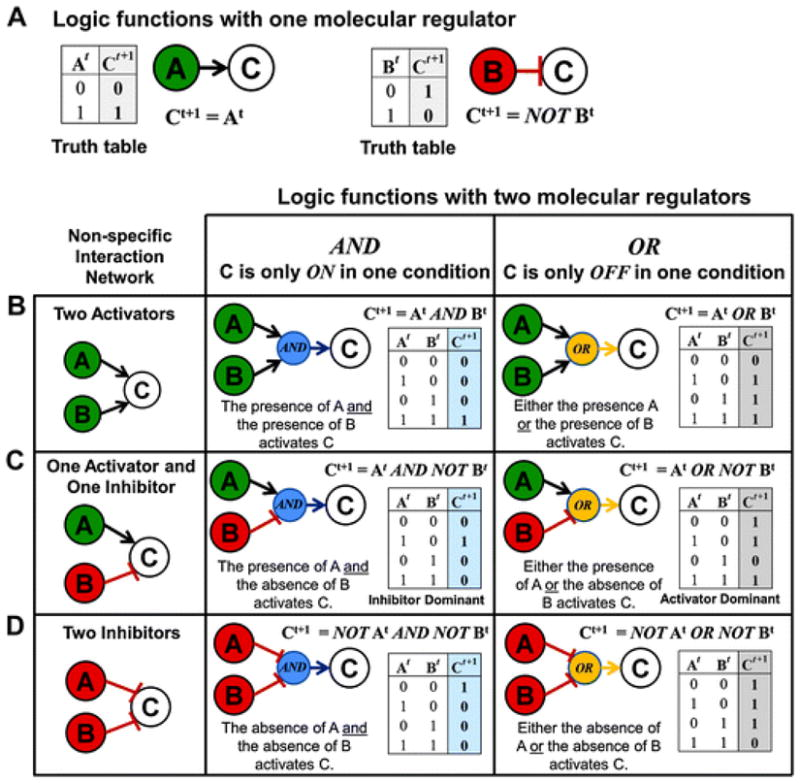
\includegraphics[scale = 0.65]{img/logicnet.jpg}
  \caption{Esempio di modellazione di interazioni tra componenti tramite
    funzioni logiche.}
  \label{fig:log}
\end{figure}
\subsection{Modelli Meccanicistici}
Come già anticipato tali modelli si limitano a descrivere \textit{sistemi
  small-scale}. Questa è la classe di approcci modellistici più complessa ed
eterogenea infatti, in primis, richiede una parametrizzazione completa delle
componenti, con un ampio range di formalismi matematici, tra cui spiccano tra
gli altri i \textbf{metodi numerici} e gli \textbf{algoritmi di simulazione
  stocasitca}. Un problema, già solo 
a questo punto, è che non si hanno spesso i dati per effettuare la
parametrizzazione in quanto i biologi/biotecnologi spesso non sono interessati a
misurarli. \\
Le simulazioni con questi modelli sono usate per studiare l'\textbf{evoluzione
  nel tempo}, quindi la dinamica, del sistema. Si usano metodi
\textit{deterministici, stocastici} e \textit{ibridi}, insieme ad una serie
infinita di altre tecniche computazionali, tra cui l'\textit{analisi di
  sensitività} o il \textit{parameters sweeping}.\\
Si arriva quindi a modelli \textit{quantitativi} e \textit{dinamici}. \\
La scelta tra metodi stocastici, solitamente più dispendiosi, e deterministici
dipende anche dal fatto che \textbf{la vita non è deterministica}. Ad esempio
modellare le interazioni tra, ad esempio tra la proteina \textit{Mdm3} e la
proteina \textit{p53}, avendo che la prima inibisce la seconda, comporta una
funzione molto pulita se studiata in modo deterministico quando in realtà, a
causa di molti fattori, non si ha tale precisione se si va a studiare cosa
accade realmente in natura. Da qui l'uso anche di \textit{modelli stocastici}.\\
La stima dei parametri resta comunque un grandissimo problema e spesso si usano
altre tecniche computazionali/modellistiche in pipeline per inferire gli stessi.
\subsection{Modelli Basati su Vincoli}
Tali modelli sono usati esplicitamente e solo per \textit{sistemi large-scale
  per reti metaboliche}. Il formalismo matematico qui usato si compone di
\textbf{matrici stechiometriche}, \textbf{algebra lineare} e tecniche di
\textbf{ricerca operativa} mentre le
simulazioni e le analisi consistono nello studiare le variazioni nelle
\textbf{distribuzione di flusso}, calcolando i valori di flusso di tutte le
reazioni metaboliche, a seconda di perturbazioni/input prefissati.\\
Non è semplice se si può dire di ottenere dei \textit{sistemi quantitativi} in
quanto si studia il comportamento ad uno \textit{steady state}.\\
Tra gli esempi di uso si hanno:
\begin{itemize}
  \item l'\textbf{ingegnerizzazione metabolica}, ovvero l'ottimizzazione, il
  design e la regolarizzazione di certe strutture/funzioni metaboliche al fine
  di ottenere un certo fenotipo metabolico
  \item studiare \textbf{bersagli di farmaci}, attraverso ad esempio lo studio
  del \textit{rewiring metabolico del cancro}
\end{itemize}
L'idea è quindi quella di:
\begin{itemize}
  \item stabilire dei \textbf{vincoli}
  \item stabilire una \textbf{funzione obiettivo} da
  \textit{massimizzare/minimizzare}
  \item determinare automaticamente la distribuzione dei flussi
\end{itemize}
Si parla di \textbf{Flux Balance Analysis (\textit{FBA})}.
\subsection{Confronto tra i Vari Approcci}
Viste queste prime piccole premesse sui quattro approcci possiamo fare qualche
piccolo confronto. \\
In primis abbiamo capito come lo studio del \textit{tempo} sia assente del tutto
nei \textit{modelli basati su interazioni} e che sia di dubbio uso nel caso dei
\textit{modelli basati su vincoli} a causa dello \textit{steady state}. Quindi
se si dovesse, ad esempio, studiare il cambio di concertazione di una certa
molecola al variare del \textit{tempo} tali approcci sarebbero da scartare a
priori.\\
Si è anche visto come, in realtà, praticamente solo i \textit{modelli
  meccanicistici} ci offrono uno studio quantitativo, al costo di una
complessità sia formale, che di dati, che computazionale molto alta e
riducendosi a studiare solo sistemi piccoli. Ne segue che:
\begin{center}
  \textit{I sistemi meccanicistici sono l'approccio modellistico migliore per
    comprendere e acquisire nuove intuizioni il funzionamento del sistema.} 
\end{center}
Nella realtà però ``avere tutto'' è un'utopia quindi non si ha un vero e proprio
vincitore in questa ``gara tra approcci modellistici'', ben riassunti nella
figura \ref{fig:app}\footnote{Bordbar, A., Monk, J., King, Z. et
  al. Constraint-based models predict metabolic and associated cellular
  functions. Nat Rev Genet 15, 107–120 (2014). https://doi.org/10.1038/nrg3643},
in quanto al variare del problema, dei dati, e di mille altri fattori potrei
aver motivi validi per preferire un approccio ad un altro.\\
\begin{figure}
  \centering
  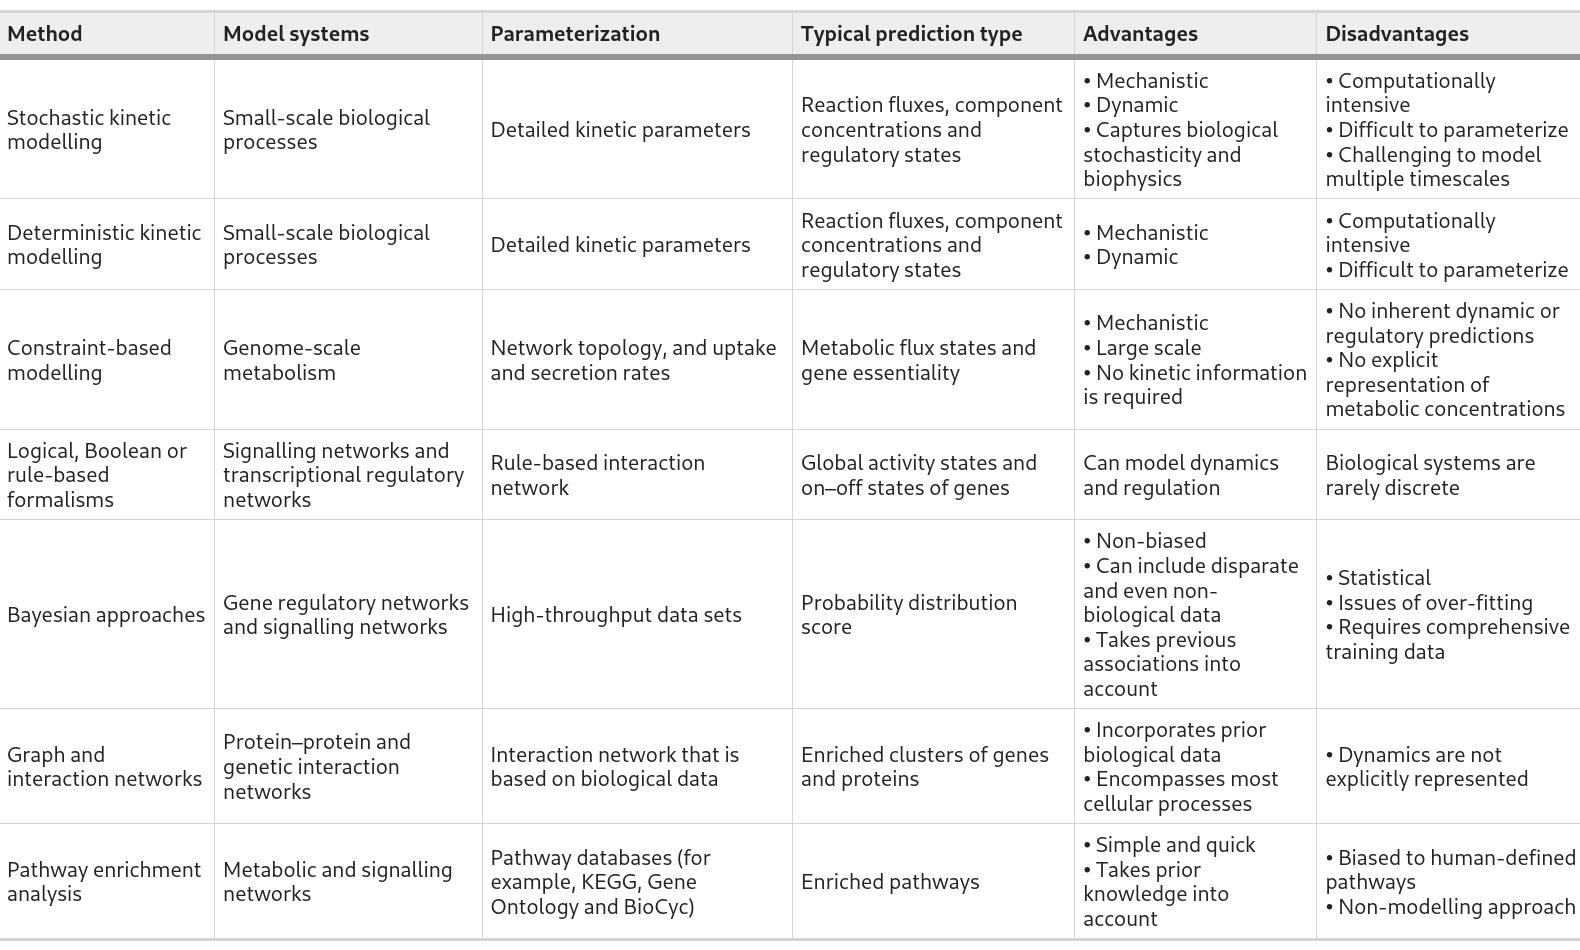
\includegraphics[width = \textwidth]{img/apptable.jpg}
  \caption{Schema riassuntivo delle caratteristiche dei vari approcci.}
  \label{fig:app}
\end{figure}
Inoltre, in questa breve introduzione, si è scoperto come ci siano moltissime
\textbf{dicotomie} in \textit{systems biology}:
\begin{itemize}
  \item \textit{top-down} e \textit{bottom-up}
  \item \textit{qualitativo} e \textit{quantitativo}
  \item \textit{statico} e \textit{dinamico}
  \item \textit{deterministico} e \textit{stocastico}
  \item \textit{discreto} e \textit{continuo} (sia in ottica di
  rappresentazione del \textit{tempo} che della numerazione delle componenti)
  \item \textit{omogeneo} e \textit{eterogeneo}
  \item \textit{a singolo volume} e \textit{multicompartamentale}
\end{itemize}
Tutte queste dicotomie rappresentano la complessità degli studi in
\textit{systems biology}.\\
Integrare i vari modelli è per lo più utopia. Fare \textit{data integration} è
già di per se uno scoglio complesso ma si aggiunge anche la difficoltà di
integrare vari formalismi matematici. Non si ha il modello ``perfetto'' ma si
può scegliere bene in base al sistema biologico da studiare, magari integrando
anche qualche (molto pochi) approccio modellistico diverso, come visibile in
figura \ref{fig:pap}\footnote{Gonçalves E, Bucher J, Ryll A, et al. Bridging the
  layers: towards integration of signal transduction, regulation and metabolism
  into mathematical models. Molecular Biosystems. 2013 Jul;9(7):1576-1583. DOI:
  10.1039/c3mb25489e. PMID: 23525368. }. Nel diagramma si segnala il paper
centrale di Karr et al.: \textit{A whole-cell computational model predicts
  phenotype from genotype}\footnote{Karr JR, Sanghvi JC, Macklin DN, et al. A
  whole-cell computational model predicts phenotype from
  genotype. Cell. 2012;150(2):389-401. doi:10.1016/j.cell.2012.05.044} cruciale
nello studio di un approccio misto per modellare il sistema un'intera cellula di
un piccolo batterio.
\begin{figure}
  \centering
  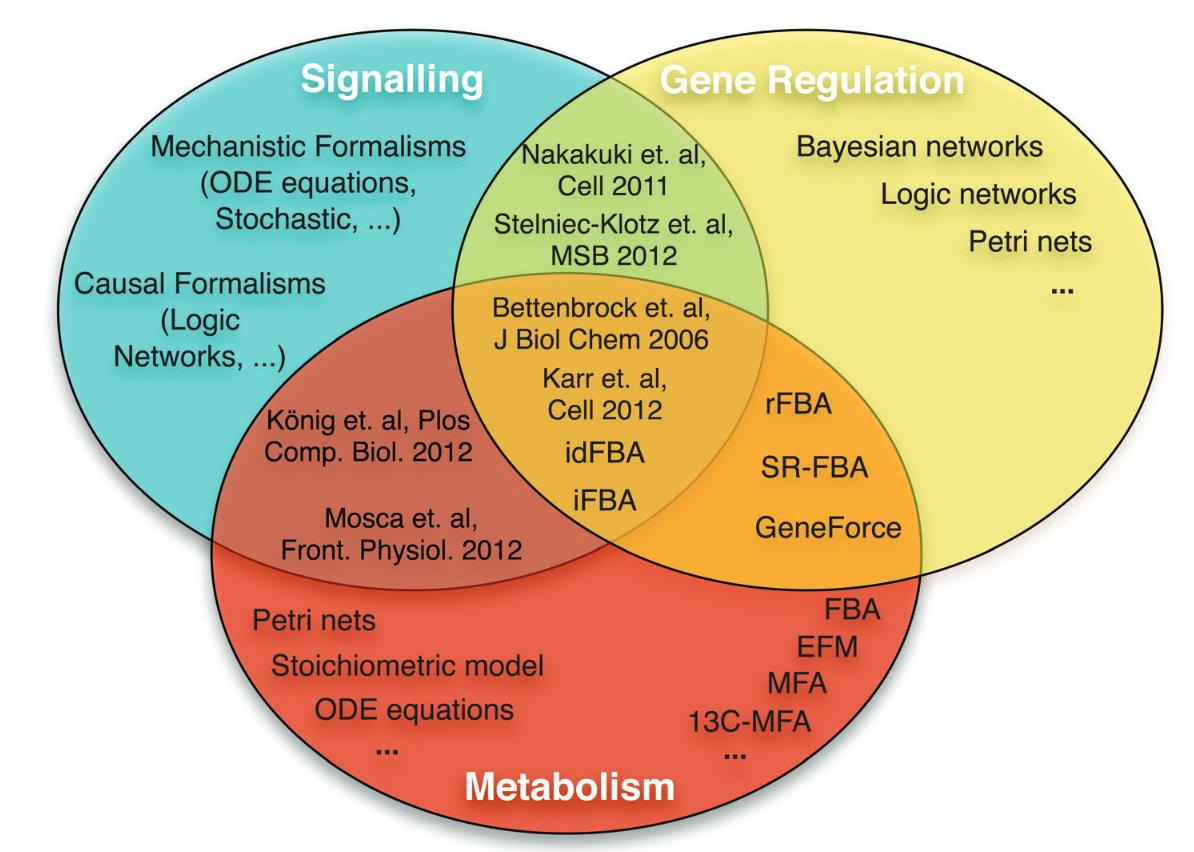
\includegraphics[scale = 0.25]{img/papers.jpg}
  \caption{Diagramma che mostra varie soluzioni modellistiche al variare del
    problema biologico}
  \label{fig:pap}
\end{figure}
\chapter{Interaction-Based Modelling}
Si parte con la descrizione della prima classe di modelli, parlando quindi della
\textbf{interaction-based modelling}.\\
Ricordiamo che tali modelli, come visibile in figura \ref{fig:appro}:
\begin{itemize}
  \item hanno un sistema di grandi dimensioni, con centinaia o migliaia di
  componenti (se non di più),
  essendo quindi \textit{modelli large-scale}
  \item presentano tendenzialmente un basso costo computazionale per le analisi
  \item hanno un basso livello di dettaglio
  \item non presentano particolari difficoltà nella misurazione dei dati
\end{itemize}
Inoltre, sempre ricordando l'introduzione alla classe, questo approccio
modellistico:
\begin{itemize}
  \item non permette propriamente di parlare di simulazioni non modellando
  \textit{tempo, localizzazione spaziale} e \textit{kinetic-rates} 
  \item indirizzano l'analisi verso lo studio topologico della rete
  \item si studiano proprietà emergenti prettamente strutturali quali la
  presenza di \textit{hubs}, misure di centralità, presenza di \textit{motifs} e
  \textit{robustezza topologica} contro certe \textit{perturbazioni}
\end{itemize}
Abbiamo quindi a che fare con \textbf{modelli qualitativi e statici}.\\
Come anticipato possiamo avere vari tipi di relazione tra i nodi della rete in
questo modello, ovvero vari tipi di \textbf{interazioni}.
\newpage
\noindent
Vediamo qualche
esempio\footnote{Merico D, Gfeller D, Bader GD. How to visually interpret
  biological data using networks. Nat Biotechnol. 2009 Oct;27(10):921-4. doi:
  10.1038/nbt.1567. PMID: 19816451; PMCID: PMC4154490.} (\textit{nel corso si
  approfondiranno solo i primi tre esempi, a livello genico e proteico}): 
\begin{itemize}
  \item \textbf{interazioni fisiche}, ovvero interazioni che si verificano tra
  biomolecole a diretto contatto. Ad esempio, le reti proteina-proteina
  con tali interazioni sono importanti in processi come la formazione di
  complessi proteici, la trasduzione del segnale e il trasporto. Sono
  tendenzialmente il caso di studio più semplice
  \item \textbf{interazioni di regolazione}, ovvero interazioni che sono eventi
  di attivazione o inibizione diretta. Ad esempio, nella regolazione
  dell'espressione genica, un fattore di trascrizione è collegato ai suoi
  bersagli da archi diretti nella rete. Quindi posso quindi avere sia
  \textit{regolazioni positive} che \textit{regolazioni negative} e non si hanno
  più \textit{interazioni fisiche}
  \item \textbf{interazioni geniche}, ovvero interazioni che connettono geni la
  cui simultanea perturbazione genetica porta a un risultato fenotipico diverso
  da quello previsto dalla combinazione di singoli effetti. Ad esempio, le
  interazioni letali sintetiche collegano i geni che influenzano debolmente la
  vitalità dell'organismo quando eliminati individualmente, ma sono letali
  quando eliminati in combinazione. Le \textit{interazioni genetiche} sono utili
  per studiare la funzione genica e per identificare complessi e pathway che
  lavorano insieme per controllare le funzioni essenziali  
  \item \textbf{relazioni di similarità}, avendo collegamenti tra oggetti
  biologici che sono \textit{simili} secondo un attributo comune. È possibile
  utilizzare molte diverse misure di somiglianza, come la somiglianza della
  sequenza proteica o la coespressione genica basata su profili trascrizionali
  correlati (avendo sia correlazioni positive che negative). Le relazioni di
  somiglianza sono utili per identificare gruppi di geni o proteine
  funzionalmente correlati. Un altro esempio è quello di studiare se, in una
  certa condizione data, si possono identificare geni indipendenti con un
  profilo di espressione (ovvero escrizione qualitativa e quantitativa
  dell’insieme dei geni trascritti in un dato momento da una cellula o da un
  tessuto, studiabile tramite, ad esempio, l'uso dei
  \textit{microarrays})
\end{itemize}
Quindi in generale si hanno tipi modelli di reti di interazioni associati ai
vari tipi di interazione (fisica, funzionale, genica, etc$\ldots$), ad
esempio\footnote{Winterbach W, Van Mieghem P, Reinders M, Wang H, de Ridder
  D. Topology of molecular interaction networks. BMC Syst
  Biol. 2013;7:90. Published 2013 Sep 16. doi:10.1186/1752-0509-7-90}: 
\begin{itemize}
  \item \textbf{Association networks}, che modellano qualsiasi tipo di relazione
  tra molecole, ad esempio legami, coespressione e somiglianze
  strutturali. Esempi di tali reti sono le \textbf{gene co-expression networks}
  e le \textbf{protein similarity networks} 
  \item \textbf{Functional networks}, che modellano le relazioni funzionali tra
  coppie di molecole (solitamente geni o proteine). Un collegamento implica che
  entrambe le componenti sono coinvolte nella stessa funzione, processo o
  fenotipo. Un esempio sono le \textbf{genetic interaction networks}
  rappresentano interazioni in cui una doppia mutazione 
  porta a un effetto epistatico (che si ha quando una coppia di alleli copre
  l'espressione fenotipica di un'altra coppia di alleli), ad esempio peggiore o
  migliore del previsto rispetto alla singola mutazione 
  \item \textbf{Protein-Protein Interaction (\textit{PPI}) networks}, che sono
  reti non dirette che modellano il legame proteico tra le componenti, che sono
  appunto proteine. Tali reti sono derivate da esperimenti ad alto rendimento
  che utilizzano tecniche come lo \textit{screening di due ibridi di lievito, la
    spettrometria di massa} e la \textit{purificazione per affinità tandem}, che
  sono metodi \textit{high-throughput}. Le
  \textbf{signaling networks} sono correlate alle \textit{reti PPI}
  ma in questo caso i collegamenti sono diretti in base al flusso di segnali
  molecolari
  \item \textbf{Transcription-Regulatory (\textit{TR}) networks}, tali reti sono
  reti bipartite con un insieme di nodi che rappresentano i geni e l'altro che
  rappresenta i \textit{fattori di trascrizione (TF, da ``transcription
    factors'')}. I \textit{TF} sono prodotti di geni (modellati da collegamenti
  \textit{gene-TF}) mentre i geni sono regolati dai \textit{TF} (modellati da
  collegamenti \textit{TF-gene}). I dati per tali reti sono derivati attraverso
  il processo di immunoprecipitazione della cromatina (detto \textit{ChIP}). Le
  \textbf{gene regulatory networks} sono correlate alle \textit{reti TR} ma
  contengono solo geni e i collegamenti rappresentano relazioni regolatorie
  indirette 
  \item \textbf{Metabolic networks}che sono reti bipartite che modellano le
  relazioni tra le reazioni chimiche che si verificano nelle cellule e i
  substrati coinvolti nelle reazioni. Spesso vengono studiate anche reti
  metaboliche ridotte e non bipartite contenenti solo metaboliti o solo
  reazioni. Parlando di metabolismo ovviamente i risultati che ottengo tramite
  queste reti sono diversi da quelli che otterrei usando, ad esempio, un
  \textit{modello basato su vincoli}
\end{itemize}
L'analisi della topologia delle reti è formata quindi da:
\begin{itemize}
  \item la \textbf{teoria dei grafi}, mediante la quale si misura il sistema
  \item le \textbf{misure di centralità}, con le quali si analizza (e non si
  simula) la rete 
  \item la \textbf{classificazione della rete}, ovvero la caratterizzazione
  della sua topologia, e la \textbf{robustezza topologica}, che sono i risultati
  delle analisi. Tali risultati possono anche corrispondere a nuovi ``insight''
  biologici 
\end{itemize}
\textit{Se aggiungiamo funzioni logiche per descrivere come cambia lo stato di
  ogni nodo nel tempo, possiamo effettuare un'analisi dinamica di una rete. Si
  hanno quindi i \emph{modelli basati sulla logica}, che aggiungono complessità,
  sia formale che computazionale, al fine di raggiungere ulteriori risultati.}
\section{Introduzione alle Reti PPI}
Prima di approfondire la classe di modelli si vede un piccolo approfondimento
sulle \textbf{Protein-Protein Interaction (\textit{PPI}) networks}, come
l'esempio in figura \ref{fig:ppn} (anche se si ricorda che la rappresentazione
di un sistema è sempre limitante), anche al
fine di capire il motivo biologico e i limiti tecnici. Gli algoritmi tipici
della teoria dei grafi ci permetteranno di studiarne la topologia.\\
\textit{Questo sarà comunque il modello più studiato in questo corso per questa
  classe}.\\ 
Ovviamente le reti sono formalizzate come dei \textbf{grafi} e, questo caso, si
hanno:
\begin{itemize}
  \item i \textit{nodi} che rappresentano le proteine
  \item gli \textit{archi}, che non sono orientati, che corrispondono alle
  interazioni di legame tra coppie di proteine
\end{itemize}
Come già anticipato le \textit{reti PPI}, più precisamente, parlando di sistemi
\textit{large-scale}, \textbf{large-scale PPI} vengono costruite a partire da
dati proteomici ottenuti tramite metodi \textit{high-throughput}, ben definiti e
con protocolli chiari (per questo non si hanno particolari challenge dal punto
di vista dell'ottenimento dati). Le \textit{reti large-scale PPI} sono però
anche caratterizzate da:
\begin{itemize}
  \item \textbf{conflitti}, in quanto tali reti sono ottenute rappresentando
  tutti i casi possibili, ignorando appunto la componente temporale. Ne segue
  quindi che, in realtà, le interfacce proteiche possono legare molte altre 
  diverse in modo mutuamente esclusivo, avendo magari che alcuni legami possono
  avvenire in modo mutuamente esclusivo in un dato tempo. Rappresentare quindi
  ``tutti i tempi'' può creare ambiguità. L'idea di togliere componenti al
  modello per evitare ambiguità non è una buona idea in quando si toglierebbe
  senso al modello (che già ha poca capacità predittiva)
  \item \textbf{complessità combinatoria} in quanto si ha un'esplosione del
  numero di complessi distinti che possono essere formati da una rete di,
  appunto, ``possibili'' legami
\end{itemize}
Il sistema è quindi \textit{statico}, non cambiando nel tempo, che non viene
nemmeno rappresentato. Il tempo non è comunque un fattore rilevante per gli
studi che si fanno su tali modelli. \\
Si hanno anche alte criticità, ad esempio:
\begin{itemize}
  \item gli archi in una \textit{rete PPI} non rappresentano necessariamente
  connessioni fisiche persistenti, ma piuttosto riassumono le possibilità di
  interazione, come già detto, e quindi si lascia spazio a:
  \begin{itemize}
    \item \textit{gaps} sia per i nodi che per gli archi, ovvero nodi/archi non
    rappresentati in quanto non si conosce una certa interazione (non ancora
    studiata nella letteratura scientifica)
    \item interazioni che sono \textit{false positive} o \textit{false negative}
  \end{itemize}
  \item le interazioni proteina-proteina nell'intera rete non si verificano,
  come detto,
  necessariamente contemporaneamente e/o utilizzando domini di legame diversi
  e/o nello stesso compartimento cellulare. In altre parole il non rappresentare
  dove accade una certa interazione può essere un problema. Si ``pone tutto allo
  stesso livello''
  \item come non si hanno informazioni temporali non si hanno nemmeno
  informazioni quantitative riguardo al funzionamento della cellula, al suo
  stato, al ciclo cellulare etc$\ldots$
  \item si rischia un bias dovuto al fatto che alcune proteine hanno più
  connessioni semplicemente perché sono meglio studiate (si parla, quando si usa
  molto la letteratura come base del modello, di \textbf{literature-curated
    networks}). Un esempio banale è pensare che la proteina \textit{p53}
  compare, a data Marzo 2019, in 94552 paper secondo PubMed (34205 direttamente
  nel titolo) mentre \textit{Snf1} 1037 volte (solo 318 nel titolo)
  \item si hanno forti limiti di modellazione. Ad esempio non si può modellare
  che una proteina interagisca con altre sse queste due ahnno prima avuto
  un'interazione tra loro (avendo che ilo massimo che posso avere è un
  ``triangolo'' nella rete)
\end{itemize}
Possiamo quindi concludere che \textbf{i risultati dello studio di una
  \textit{rete PPI} (ma anche delle altre reti tipiche
  dell'\textit{interaction-based modelling}) non sono sempre così affidabili}.
\section{La Teoria dei Grafi}
Lo studio dei \textbf{grafi} è centrale in vari problemi/tecnologie comuni,
dal web ai social, dalle reti di collaborazione (pensando ad esempio al
\textit{erd\"{o}s number}) a ipotesi come la famosa
\textit{ipotesi dei sei gradi di separazione} che dimostra (come visto sia nel
collegare attori a Kevin Bacon che con lo studio del 1967 più ``accademico''
dello psicologo Stanley Milgram)
come si abbiano di media sei passaggi per collegare due persone a caso nel
mondo. Si parla infatti spesso della \textbf{teoria del mondo piccolo}, che è
appunto una teoria matematica e sociologica che sostiene che tutte le reti
complesse presenti in natura sono tali che due qualunque nodi possono essere
collegati da un percorso costituito da un numero relativamente piccolo di
collegamenti.
\begin{definizione}
  Si definisce formalmente un \textbf{grafo} $G$ come una coppia di insiemi:
  \[G=\langle V, E\rangle\]
  dove:
  \begin{itemize}
    \item $V=\{v_1,\ldots,v_n\}$ è l'insieme dei \textbf{nodi}, di cardinalità
    $n$ 
    \item $E\subseteq V\times V$ è l'insieme degli \textbf{archi}, di
    cardinalità $m$. Si ha che $E=\{e_1,\ldots,e_m\}$, dove un generico arco
    $e_k=(v_i,v_j)$ con $k=1,\ldots,m$, è definito come una coppia di vertici
    $v_i,v_j\in V$ 
  \end{itemize}
\end{definizione}
\begin{definizione}
  In un grafo si definisce \textbf{nodo isolato} un nodo che non è connesso a
  nessun altro nodo. 
\end{definizione}
\begin{definizione}
  In un grafo si definisce \textbf{cappio} un arco tra un nodo e se stesso.
\end{definizione}
\begin{definizione}
  In un grafo $G=\langle V,E\rangle$ si definisce \textbf{percorso/cammino} come
  una sequenza finita o infinita 
  di archi che unisce una sequenza di vertici. Dati quindi due nodi $v_1,v_n\in
  V$ un cammino da $v_1$ a $v_n$ un cammino è una sequenza di nodi: 
  \[(v_1,v_2, \ldots, v_n) \mbox{ tali che }\forall i =1,2,\ldots,
    n-1,\,\,\exists \,e=(v_1, v_{i+1})\in E\]
  Se il vertice di partenza coincide con quello di fine si parla di
  \textbf{ciclo}, quindi $v_1=v_n$. \\
  Ovviamente tra due nodi possono avere distinti cammini.
\end{definizione}
Il concetto di \textit{cammino} e il concetto di \textit{ciclo} assumono
particolare rilevanza in biologia. I \textit{cicli} servono, ad esempio, per
rappresentare i \textit{feedback} mentre i \textit{cammini}, ad esempio, per le
\textit{vie di trasduzione del segnale} dove si parte da un recettore
transmembrana per poi attivare una catena di reazioni.
\begin{definizione}
  Si definisce \textbf{grafo connesso} un grafo dove esiste un percorso tra ogni
  coppia di vertici. In caso contrario si parla di \textbf{grafo non connesso}.
\end{definizione}
\begin{definizione}
  Si definisce \textbf{grafo completo} o \textbf{grafo completamente connesso}
  un grafo, di $n$ nodi, dove ogni nodo è collegato ai rimanenti $n-1$ nodi.
\end{definizione}
\begin{definizione}
  Si definisce \textbf{grafo totalmente sconnesso} un grafo che non presenta
  archi.  
\end{definizione}
\begin{definizione}
  Due nodi $v_i$ e $v_j$ si dicono \textbf{adiacenti} se esiste un arco, diretto
  o indiretto, $e=(v_i, v_j)$.
\end{definizione}
\begin{definizione}
  Dato un nodo $v$ in un \textit{grafo indiretto} si definisce
  \textbf{grado/connettività/degree} come il 
  numero di 
  nodi adiacenti ad esso. Tale valore solitamente si indica con $k_v$, che è
  ovviamente un numero intero non negativo. Qualora ci sia un cappio esso conta
  doppio.\\
  Un \textbf{nodo isolato} presenta un grado nullo.
\end{definizione}
\begin{definizione}
  Dato un \textit{grafo diretto} si definiscono:
  \begin{itemize}
    \item \textbf{indegree} di un nodo $v$ come il numero di archi entranti in $v$
    \item \textbf{outdegree} di un nodo $v$ come il numero di archi uscenti da $v$
  \end{itemize}
  \textit{In letteratura ha volte si definisce
    \textbf{grado/connettività/degree} in un grafo diretto come la somma di
    \emph{indegree} e \emph{outdegree}}.
\end{definizione}
Nella modellazione di sistemi biologici mediante questa classe di modelli è
interessante notare come si possa passare da un grafo connesso ad uno non
connesso dopo l'influenza di una \textit{perturbazione} sul sistema, che
influisce sulle interazioni (e quindi sugli archi) tra le componenti. Tali
cambiamenti hanno forte valenza dal punto di vista biologico in quanto se un
sistema è propenso a produrre un grafo disconnesso dopo una perturbazione, come
ad esempio in figura \ref{fig:conn}, allora è un sistema che è in generale
propenso a ``fallire''. 
\begin{figure}
  \centering
  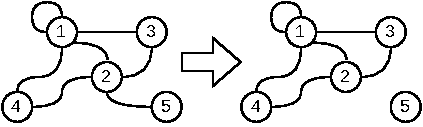
\includegraphics[scale = 1.35]{img/ncon.pdf}
  \caption{Esempio di passaggio da \textit{grafo connesso} a \textit{grafo non
      connesso} dopo un'ipotetica perturbazione, che produce il \textit{nodo
      isolato} etichettato con 5.} 
  \label{fig:conn}
\end{figure}
\begin{definizione}
  Si definisce \textbf{grafo orientato} un grafo dove ogni arco consiste in una
  \textbf{coppia orientata} di vertici, altrimenti si parla di \textbf{grafo non
    orientato}. Formalmente si ha quindi, per un \textit{grafo orientato}, con
  $v_1,v_2\in V$: 
  \[e=(v_1,v_2)\neq e'=(v_2,v_1)\]
  In tal caso, a livello grafico, gli archi sono rappresentati mediante frecce.
\end{definizione}
In questa classe modellistica si hanno:
\begin{itemize}
  \item \textbf{grafi orientati} per \textit{gene regulatory networks} e
  \textit{signal transduction networks}
  \item \textbf{grafi non orientati} per \textit{reti PPI}
\end{itemize}
\begin{definizione}
  Dato un grafo $G=\langle V, E\rangle$ si definisce $S$ come
  \textbf{sottografo} di $G$ come una coppia di insiemi:
  \[S=\langle V', E'\rangle\]
  dove:
  \begin{itemize}
    \item $V'\subseteq V$
    \item $E'\subseteq E$
  \end{itemize}
\end{definizione}
Possiamo quindi dire che, riprendendo la figura \ref{fig:conn}, mediante una
\textit{perturbazione}, si ottiene un sottografo del grafo di partenza. \\
I sottografi sono molto utili per studiare ``caratteristiche'' di forte
interesse biologico, rappresentate appunto da sottografi\footnote{Winterbach W,
  Van Mieghem 
  P, Reinders M, Wang H, de Ridder D. Topology of molecular interaction
  networks. BMC Syst Biol. 2013;7:90. Published 2013 Sep
  16. doi:10.1186/1752-0509-7-90}:  
\begin{itemize}
  \item \textbf{modules} che sono sono sottografi indotti la cui densità di
  archi è elevata rispetto al resto del grafo. Questa non è una vera e propria
  definizione in quanto al natura dei \textit{modules} varia dal contesto e
  dall'algoritmo utilizzato per scoprirli 
  \item \textbf{motifs} che sono piccoli sottografi, solitamente di tre o
  quattro nodi, 
  la cui sovrarappresentazione o sottorappresentazione può indicare che le loro
  strutture sono ``importanti'' o ``dannose'' per il sistema. Di solito, vengono
  contati 
  tutti i \textit{motifs} distinti in una rete, ottenendo una \textit{motif
    signature} per la 
  rete che può quindi essere confrontata con le firme, ottenute campionando da
  un modello nullo di rete casuale appropriato, per determinare la 
  sovrarappresentazione o sottorappresentazione. Le \textit{motif
    signature} possono essere usate per caratterizzare le reti stesse
  \item \textbf{graphlets} che sono simili ai \textit{motifs} ma sono
  \textit{completamente connessi}. Anch'essi vengono utilizzati per costruire
  firme che catturano le caratteristiche locali di una rete  
\end{itemize}
\textbf{Questi argomenti verranno approfonditi più avanti, queste sono solo le
  ``definizioni'' recuperate nel paper indicato.}\\
Torniamo a parlare di della nozione di \textbf{grado}.
\begin{definizione}
  Si definisce \textbf{distribuzione dei gradi/degree distribution} come la
  distribuzione di 
  probabilità dei gradi dei nodi sull'intera rete. Tale distribuzione, denotata
  con $P(k)$, quindi è la
  probabilità che un certo nodo abbia grado esattamente pari a $k$. Tale
  probabilità si ottiene contando il numero di nodi del grafo, denotati $N(k)$,
  che presentano grado $k$ e dividendo tale valore per il numero totale di nodi
  del grafo, che indichiamo con $N=|V|$. Si ha quindi:
  \[P(k)=\frac{N(k)}{N},\,\,k=1,2,\ldots\]
  Avendo una distribuzione di probabilità ne segue che:
  \[\sum_{i=1}^{k_{max}} P(i)=1\]
\end{definizione}
La \textbf{degree distribution} ci permette di classificare un grafo, anche
solo plottando con un istogramma i valori di $P(k)$ al variare di $k$
stesso. Ad esempio qualora si avesse un picco nel plot di tali valori allora si
avrebbe che la rete ha un ``grado caratteristico'' (estremizzando l'esempio
magari si ha una rete dove tutti i nodi hanno grado $k=2$) e quindi non si hanno
nodi fortemente connessi, con alto \textit{degree}. Questo tipo di analisi non
può essere fatta ``visivamente'' su reti reali ma ci si deve per forza affidare
a conti precisi o al più plot della distribuzione stessa. Da tali studi posso
estrarre alcune informazioni, ad esempio:
\begin{itemize}
  \item i nodi con $k=0$, ovvero i nodi isolati possono rilevare che ci sono
  probabilmente informazioni mancanti, falsi negativi etc$\ldots$ mentre il
  valore di $P(0)$ mi dice la probabilità stessa che un qualsiasi nodo della
  rete sia un nodo isolato
  \item i nodi con un $k$ elevato sono tendenzialmente molto pochi e sono i
  cosiddetti \textbf{hubs}, che hanno un ruolo chiave nello studio di
  \textit{reti large-scale} 
\end{itemize}
Al fine di rappresentare i vari valori si usa un piano cartesiano (spesso per
necessità rappresentato in \textit{scala logaritmica}) dove:
\begin{itemize}
  \item l'asse delle $x$ è formato dai valori di $k$
  \item l'asse delle $y$ è formato dai valori di $P(k)$
\end{itemize}
Rappresentando tutte le varie coppie $\langle k,P(k)\rangle$ si ottiene una
``forma'' che è la cosiddetta \textbf{power-law degree distribution} (che
rappresenta la relazione funzionale tra $k$ e $P(k)$ dove una variazione
relativa in una delle due quantità si traduce in una variazione relativa
proporzionale nell'altra quantità, indipendentemente dalla dimensione iniziale
delle due quantità, avendo quindi che una quantità varia come potenza di
un'altra). Lo studio della \textit{power-law degree distribution} è spesso
essenziale nello studio di sistemi biologici.\\
Sempre restando sullo stesso discorso si è notato che in molte reti se si ha un
nodo $v_i$ connesso con un nodo $v_j$, che a sua volta è connesso al nodo $v_h$,
allora è altamente probabile che $v_i$ sia anch'esso collegato al nodo
$v_h$. Questo \textbf{fenomeno di clusering} può essere quantificato usando il
cosiddetto \textbf{coefficiente di clustering}.
\begin{definizione}
  Dato un nodo $v$ si definisce il \textbf{coefficiente di clustering} del nodo
  $v$, denotato con $C_v$, come il numero di archi che connettono nodi adiacenti
  a $v$ diviso il numero totale delle possibili connessioni che si avrebbero tra
  i nodi adiacenti a $v$. Formalmente:
  \[C_v=\frac{2N_v}{k_v(k_v-1)}\]
  infatti si hanno:
  \begin{itemize}
    \item $N_v$ come numero di archi che connettono coppie di nodi adiacenti a
    $v$. Questo valore è facilmente contabile avendo il grafo
    \item $\frac{k_v(k_v-1)}{2}$, parlando di \textit{grafo indiretto}, come
    numero di tutti i possibili archi tra 
    coppie di nodi adiacenti a $v$, che ha grado $k_v$, un valore conosciuto
  \end{itemize}
  Si osserva inoltre che, ricordando che alla fine si ha a che fare con la
  misura di probabilità di quanto sia probabile che si abbia o meno un cluster
  che include il nodo $v$:
  \[0\leq C_v\leq 1\]
\end{definizione}
\begin{esempio}
  Vediamo un semplice esempio che mostra come varia il \textit{coefficiente di
    clustering}. Si studia, nel dettaglio, il valore $C_5$ nei seguenti grafi:
  \begin{figure}[H]
    \centering
    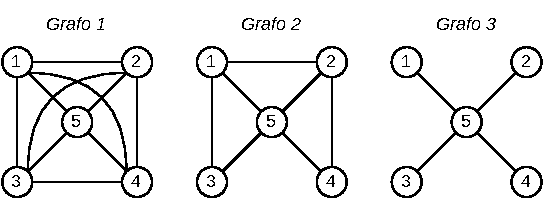
\includegraphics[scale = 1.3]{img/clus.pdf}
  \end{figure}
  In tutti i casi si ha $k_5=4$ ma:
  \begin{itemize}
    \item nel \textit{Grafo 1} si ha $N_5=6$ e $C_5=\frac{12}{12}=1$ e infatti
    il nodo $5$ è sicuramente in cluster
    \item nel \textit{Grafo 2} si ha $N_5=3$ e $C_5=\frac{6}{12}=0.5$
    \item nel \textit{Grafo 3} si ha $N_5=0$ e $C_5=\frac{0}{12}=0$ e infatti il
    nodo $5$ non è sicuramente in cluster
  \end{itemize}
\end{esempio}
Questo tipo di coefficiente è utile soprattutto nel caso di \textit{grafi
  indiretti}. Nel caso di \textit{grafi diretti} bisogna invece ragionare in
ottica di \textit{indegree} e \textit{outdegree}.\\
Un caso limite interessante in ottica di \textit{coefficiente di clustering} è
quello della \textbf{clique}.
\begin{definizione}
  Si definisce \textbf{clique (\textup{cricca})} di un \textit{grafo non
    orientato}
  $G=\langle V,E\rangle$ come un sottoinsieme $V'\subseteq V$ di vertici tale
  che: 
  \[(v_1,v_2)\in E,\,\,\forall \,v_1,v_2\in V'\]
  quindi un sottoinsieme di vertici con solo vertici collegati da un arco.
\end{definizione}
Il caso della \textit{clique} è quindi il ``caso migliore'' parlando del
fenomeno del clustering.\\
Il singolo \textit{coefficiente di clustering} di un nodo comunque non è di
particolare interesse se preso in modo isolato, in quanto si vuole classificare
l'intera rete.
\begin{definizione}
  Si definisce il \textbf{coefficiente di clusering medio}, denotato con
  $\langle C\rangle$, il valore medio di tutti i \textit{coefficienti di
    clusering} dei nodi del grafo.
\end{definizione}
Il \textit{coefficiente di clusering medio} permette di caratterizzare la
tendenza complessiva dei nodi di una rete a formare gruppi o cluster. Questo è
quindi un valore che ci permette di caratterizzare la topologia di una rete.
\begin{definizione}
  Si definisce la funzione $C(k)$, che potremmo chiamare ``\textbf{average
    clustering distribution}'' o \textbf{average clustering coefficient}, come
  la media dei \textit{coefficienti di 
    clusering} di tutti i nodi di grado pari a $k$ nella rete.
\end{definizione}
Il valore $C(k)$ quindi fornisce un'indicazione del carattere
modulare/gerarchico di una rete, ovvero l'esistenza di sottografi/sottoreti
caratterizzati da nodi fortemente collegati internamente, che presentano scarse
connessioni con altre parti della rete.
\begin{definizione}
  Si definisce la \textbf{lunghezza del cammino} tra due nodi $v_1$ e $v_n$ come
  il numero di archi che si hanno nel cammino.\\
  Si definisce \textbf{cammino minimo}, notando che potrebbe non essere unico,
  un cammino di lunghezza minima tra due nodi. 
\end{definizione}
Anche la nozione di \textit{lunghezza del cammino}  ha un ruolo centrale nella
modellazione di sistemi biologici. Basti pensare, in modo comunque approssimato
e semplicistico, che più è lungo il cammino e più sono le interazioni biologiche
e quindi, ad esempio, più energia è richiesta alla cellula. Infatti normalmente
la natura ha fatto sì che ogni ``operazione biologica'' venga fatta nel modo
meno dispendioso possibile, quindi, ricollegando la modellazione a grafo,
mediante \textit{cammini minimi}. Nella realtà si vedrà il concetto di
\textbf{ridondanza} in quanto si hanno vari modi, nel mondo biologico, per
ottenere lo stesso risultato anche se con ``cammini'' di lunghezza diversa
(magari per casi, ad esempio, in cui alla cellula conviene
``temporeggiare''). Inoltre magari ad un percorso più lungo può comunque
corrispondere un dispendio energetico minore. In ogni casa l'aggiunta di
\textbf{pesi} al grafo permette 
una modellazione leggermente più precisa, potendo rappresentare ad esempio, i
``costi'' delle reazioni etc$\ldots$\\
Un'altra cosa interessante da notare nella maggior parte delle reti è che
esiste un cammino relativamente breve tra qualsiasi coppia di nodi e la
lunghezza media di tale cammino è proporzionale al logaritmo della dimensione
della rete, quindi al numero totale di nodi. Questa è la cosiddetta
\textbf{small world property} che sembra caratterizzare la maggior parte delle
reti complesse, comprese \textit{reti metaboliche} e \textit{reti PPI}.
\begin{definizione}
  Si definisce un \textbf{grafo pesato} $G=\langle V,E\rangle$ come un grafo a
  cui viene associata anche una \textbf{funzione di peso} $w$:
  \[w:E\to\mathbb{R}\]
\end{definizione}
Esistono, oltre a quelle già citate, anche altre metriche di studio, tra
cui\footnote{Winterbach W, Van Mieghem P, Reinders M, Wang H, de Ridder
  D. Topology of molecular interaction networks. BMC Syst
  Biol. 2013;7:90. Published 2013 Sep 16. doi:10.1186/1752-0509-7-90}: 
\begin{itemize}
  \item ulteriori \textbf{metriche per i cammini} come il \textit{cammino
    minimo} su \textit{grafi pesati} o il \textit{cammino minimo medio} tra
  ogni coppia di nodi
  \item la \textbf{metrica di centralità} fornisce una classifica dei nodi in
  base alla loro "importanza". La versione più semplice sfrutta appunto il grado
  di un nodo per misurarne la centralità, parlando quindi di \textbf{degree
    centrality}. Un'alternativa è la \textbf{closeness centrality} che è il
  reciproco della somma dei cammini più brevi verso tutti gli altri nodi (cioè
  un nodo la cui \textit{closeness centrality} è alta è vicino a molti
  nodi). Un'ulteriore metrica è la \textbf{betweenness centrality} ovvero la
  frazione di cammini minimi che passano attraverso un nodo. Tra le metriche più
  elaborate si annoverano la \textbf{centralità per autovettori} e il
  \textbf{pagerank} che sono misure della frequenza con cui si arriva a un nodo
  quando si esegue una \textit{random walk} su una rete.  
\end{itemize}
\textbf{Queste non sono comunque metriche solitamente utili per la
  caratterizzazione della topologia di una rete}.
\begin{definizione}
  Si definisce un grafo $G=\langle V,E\rangle$, orientato o meno, come un
  \textbf{grafo bipartito} se:
  \begin{itemize}
    \item l'insieme dei nodi $V$ è in realtà l'unione di due sottoinsiemi di
    nodi $V_1$ e $v_2$, ovvero $V=V_1\cup V_2$, tali che la loro intersezione è
    nulla, ovvero $V_1\cap V_2=\emptyset$
    \item data la prima premessa si ha che ogni arco del grafo connette solo un
    nodo in $V_1$ ad un nodo in $V_2$
  \end{itemize}
  Ad esempio potremmo avere questi casi, dove i primi due grafi sono bipartiti
  (come evidenziato anche a livello visivo dai colori che identificano le
  partizioni) a differenza del terzo (a causa dell'arco in rosso):
  \begin{figure}[H]
    \centering
    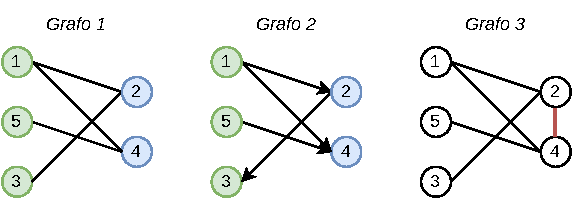
\includegraphics[scale = 1.3]{img/bip.pdf}
  \end{figure}
  Potenzialmente si possono anche avere \textbf{grafi tripartiti}, con 3
  partizioni, o in generale \textbf{grafi multipartiti} con $m$ partizioni.
\end{definizione}
\newpage
Un esempio d'uso dei \textit{grafi bipartiti} sono le \textbf{human desaesome
  networks}, come ad esempio\footnote{Goh, Kwang-Il, et al. "The
  human disease network." Proceedings of the National Academy of Sciences 104.21
  (2007): 8685-8690.}:
\begin{figure}[H]
  \centering
  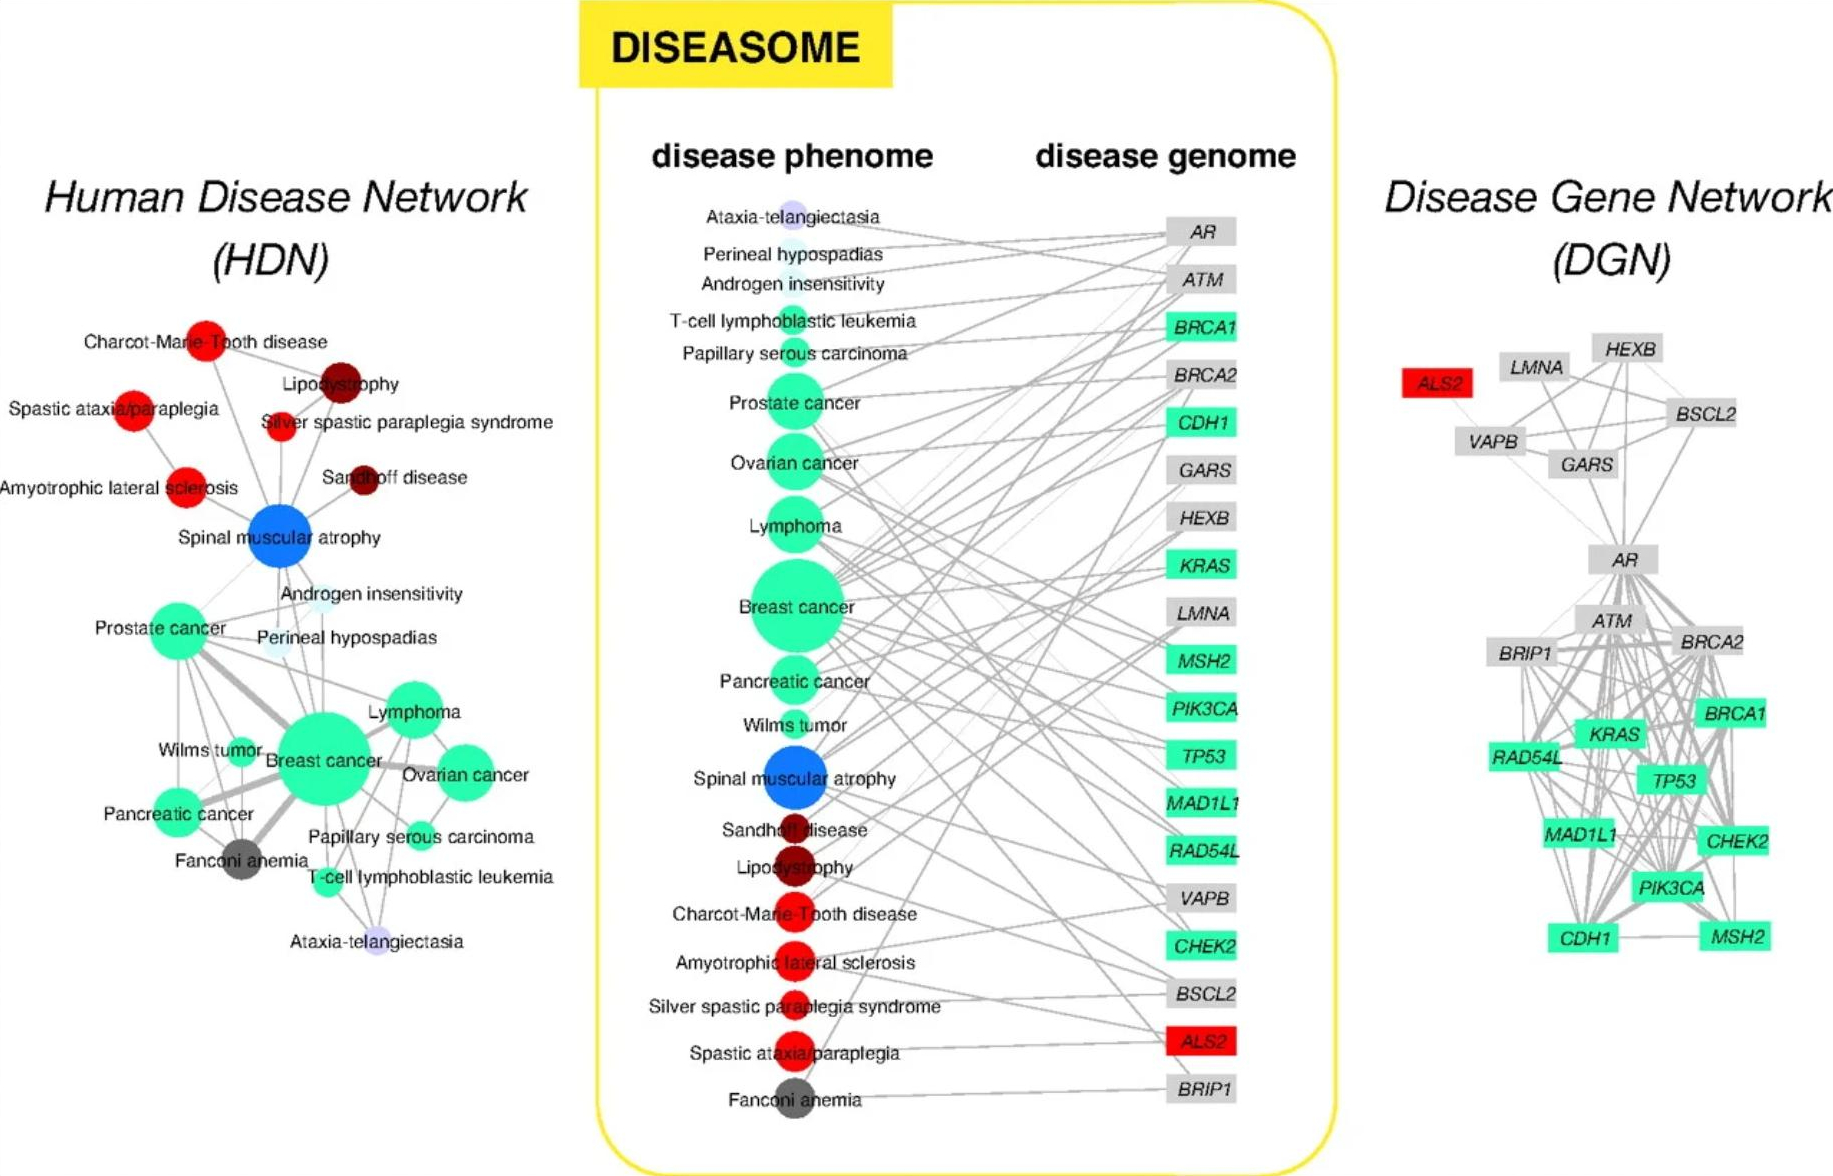
\includegraphics[scale = 0.7]{img/bi.jpg}
  \label{fig:mbip}
\end{figure}
Nella figura si hanno appunto due partizioni: 
\begin{itemize}
  \item un sottoinsieme di nodi per i geni
  \item un sottoinsieme di nodi per le malattie
\end{itemize}
Banalmente quindi un nodo che rappresenta una malattia è legato a un nodo che
rappresenta un gene se è noto che una
mutazione di quel gene induce l'insorgenza di quella malattia. A supporto posso
inoltre avere due ulteriori reti solo per i geni e solo per le malattie.\\
Un esempio di rete basata su un \textit{grafo multipartito} è, ad esempio, una
\textbf{drug-target protein network}, come quella proposta da
Nacher visualizzabile in figura
\ref{fig:mbip}\footnote{Nacher, J., Akutsu, T. Structural controllability of
  unidirectional bipartite networks. Sci Rep 3, 1647
  (2013). https://doi.org/10.1038/srep01647}.
\begin{figure}
  \centering
  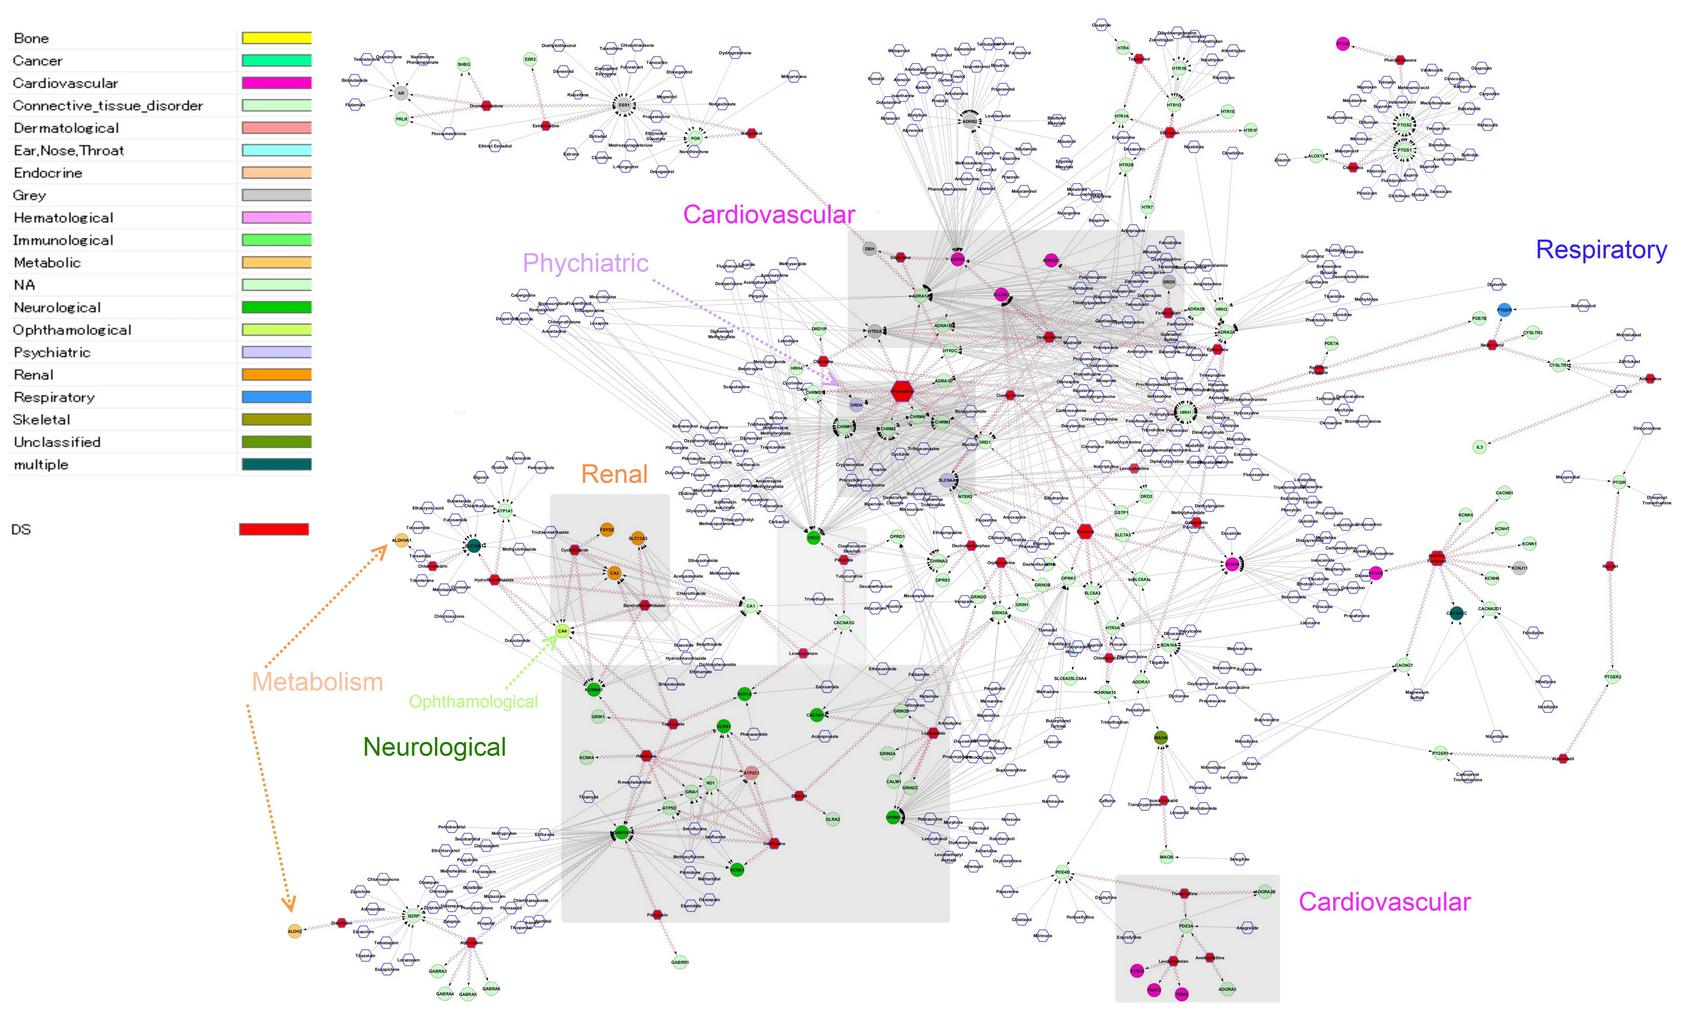
\includegraphics[scale = 0.22]{img/multi.jpg}
  \caption{Esempio di \textit{drug-target protein network}, rappresentata
    mediante \textit{grafo multipartito}.}  
  \label{fig:mbip}
\end{figure}
\newpage
Un esempio invece di rete tripartita può essere la rappresentazione di un
\textit{pathway metabolico}\footnote{Réka Albert; Scale-free networks in cell
  biology. J Cell Sci 1 November 2005; 118 (21): 4947–4957. doi:
  https://doi.org/10.1242/jcs.02714}: 
\begin{figure}[H]
  \centering
  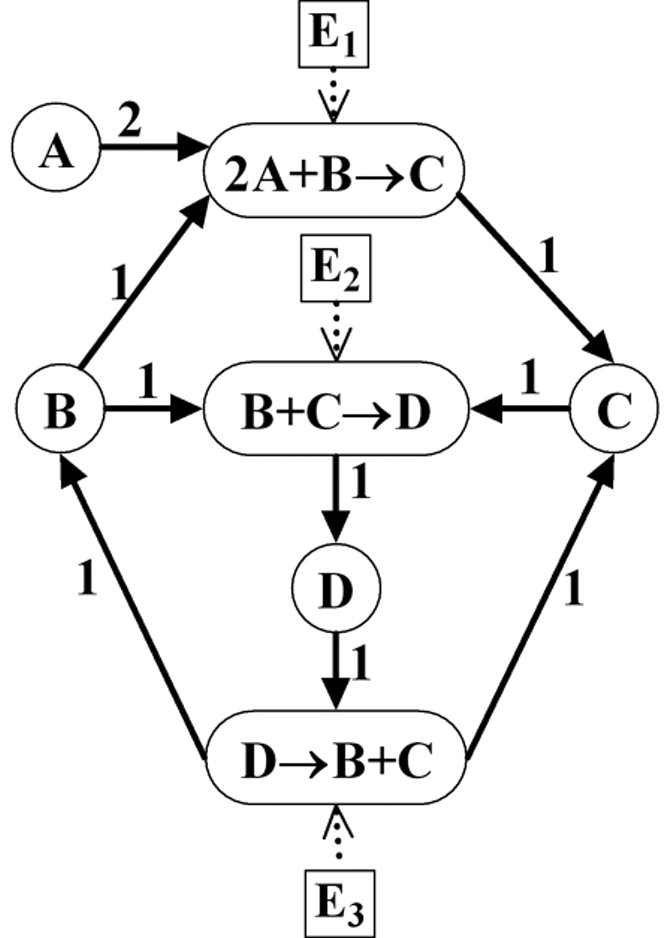
\includegraphics[scale = 0.22]{img/tri.jpg} 
\end{figure}
dove si hanno tre tipologie di nodo:
\begin{enumerate}
  \item nodi per i \textit{reagenti} (nell'immagine rappresentati da cerchi)
  \item nodi per le \textit{reazioni} (nell'immagine rappresentate da ovali)
  \item nodi per gli \textit{enzimi} (nell'immagine rappresentati da quadrati)
\end{enumerate}
Si hanno inoltre due tipologie di archi:
\begin{enumerate}
  \item le linee solide per rappresentare il \textit{mass flow},
  ovvero il \textit{tasso di turnover} delle molecole attraverso una via
  metabolica, tasso che serve ad indicare il dispendio energetico (???)
  \item le linee tratteggiate per la \textit{catalisi}, ovvero fenomeno chimico
  attraverso il quale la velocità di una reazione chimica subisce delle
  variazioni per l'intervento di una sostanza (o una miscela di sostanze) detta
  catalizzatore, che non viene consumata dal procedere della reazione
  stessa\footnote{\url{https://it.wikipedia.org/wiki/Catalisi}} 
\end{enumerate}
Inoltre i pesi degli archi indicano i \textit{coefficienti stechiometrici}, che
rappresentano infatti il rapporto tra le moli delle diverse sostanze, dei
reagenti.  \\
Ovviamente l'uso delle reti in ambito biologico può essere espanso, considerando
ad esempio i legami tra più reti, che rappresentano vari livelli, ad esempio:
\begin{itemize}
  \item \textit{reti sociali}, da usare comunque con cautela a causa della loro
  alta probabilità di portare \textit{falsi positivi/negativi} anche se possono
  rappresentare informazioni importanti. Ormai si tende comunque a preferire il
  dato del singolo paziente, puntando alla \textit{medicina personalizzata} in
  quando ``la media tra i pazienti'' raramente è un dato utile. Esse
  possono rappresentare legami 
  famigliari, vicinanza tra persone, informazioni sui luoghi in cui si vive
  etc$\ldots$ 
  \item \textit{disease networks}
  \item \textit{reti metaboliche}
  \item \textit{reti PPI}
  \item \textit{reti di regolazione genica}
  \item $\ldots$
\end{itemize}
I vari livelli sono ovviamente connessi a vicenda ma non sempre è facile
studiare tali connessioni a causa della mancanza di dati etc$\ldots$\\
Altri esempi interessanti di uso sono le \textbf{reti in ecologia}, come, ad
esempio, lo 
studio di Faust e Raes\footnote{Faust, K., Raes, J. Microbial interactions: from
  networks to models. Nat Rev Microbiol 10, 538–550
  (2012). https://doi.org/10.1038/nrmicro2832} dove si studiavano le
\textit{interazioni microbiche}, tra cui il parassitismo, il mutualismo la
competizione etc$\ldots$ tramite appunto delle reti.\\
Un uso recente delle reti è anche quello nelle \textbf{neuroscienze}, per
capire, durante una malattia, cosa non stia funzionando bene nel cervello. Un
esempio è lo studio di Chennu, Srivas et al.\footnote{Chennu, Srivas, et
  al. "Spectral 
  signatures of reorganised brain networks in disorders of consciousness." PLoS
  computational biology 10.10 (2014): e1003887.} dove si è sfruttata la
relazione tra reti e funzionalità del cervello per identificare quali aree del
cervello/funzioni del cervello funzionassero male in pazienti in stato
vegetativo e pazienti 
minimamente coscienti, facendo il paragone con vari soggetti controllo
sani. Sono stati usati anche i concetti di grado etc$\ldots$ nello studio.
\section{Tipologie di Reti}
Un aspetto fondamentale nello studio delle reti è inoltre quello che sia la
\textit{degree distribution} $P(k)$ che il \textit{average clustering
  coefficient} $C(k)$ sono \textbf{indipendenti} dalla grandezza delle rete e
possono essere usati per identificare caratteristiche generali e classificare le
reti stessi. Tra le tipologie più importanti abbiamo:
\begin{itemize}
  \item \textbf{random network}
  \item \textbf{scale-free network}
  \item \textbf{hierarchical network}
\end{itemize}
Ad ogni tipologia ovviamente corrisponde un certo insieme di caratteristiche,
come ad esempio le seguenti catalogate da Mitchell\footnote{Mitchell,
  Melanie. (2006). Field review: Complex systems: Network thinking. Artificial
  Intelligence. 170. 1194-1212. 10.1016/j.artint.2006.10.002.}:
\begin{figure}[H]
  \centering
  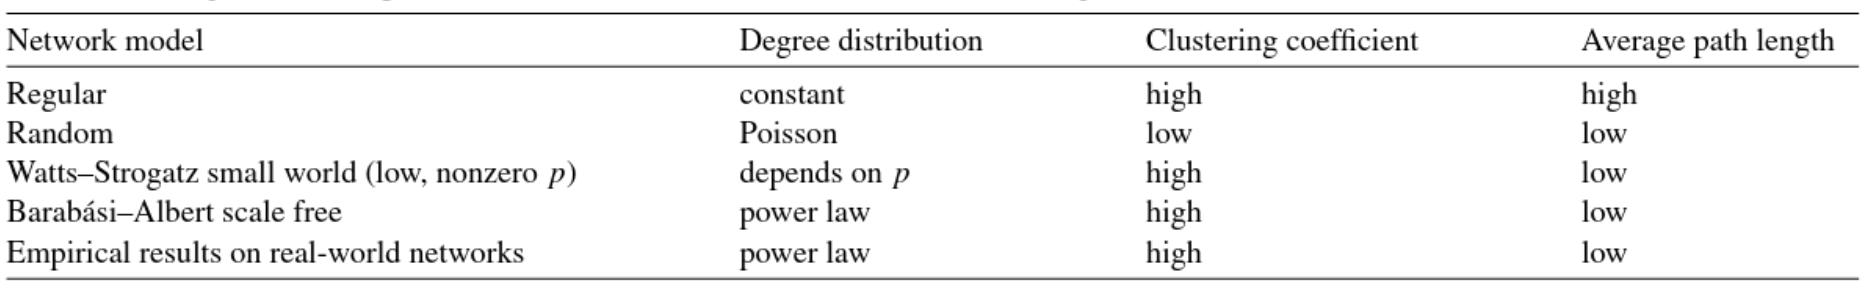
\includegraphics[width = \textwidth]{img/net.jpg} 
\end{figure}
\newpage
\subsection{Random Network}
Si comincia parlando delle \textbf{random network}, dette anche
\textbf{Erd\"{o}s-Rényi model}, dal nome di coloro che le formalizzarono nel
1960.\\
Si hanno quindi le seguenti caratteristiche principali per una \textit{random
  network}: 
\begin{itemize}
  \item la rete è \textbf{statisticamente omogenea}, infatti la maggior parte
  dei nodi ha circa lo stesso numero di archi incidenti che quindi è vicino al
  grado medio della rete $\langle k \rangle$
  \item la \textit{degree distribution} segue una \textbf{distribuzione di
    Poisson}, avendo quindi che si hanno davvero pochissimi nodi con un numero
  di archi incidenti maggiore o minore del valore medio. Si ha quindi,
  graficamente, una ``campana'' molto stretta sulla media del grado di tutti i
  nodi della rete,
  come visibile in figura \ref{fig:pois}\footnote{Réka Albert; Scale-free
    networks in cell biology. J Cell Sci 1 November 2005; 118 (21):
    4947–4957. doi: https://doi.org/10.1242/jcs.02714} 
  \item non si ha \textbf{modularità intrinseca}, non avendo quindi
  \textit{moduli} e avendo che $C(k)$è indipendente dal valore di $k$. Si hanno
  quindi pochi cluster
  \item sono caratterizzate dalla \textbf{small world property}
\end{itemize}
In merito all'ultimo punto bisogna formalizzare meglio quanto già
anticipato. Quando tale proprietà è garantita si ha che la lunghezza media di
un cammino tra due nodi è proporzionale a $\log |V|$, assicurando quindi alta
velocità di trasmissione delle ``informazioni'' nella rete. Questo è necessario
nei sistemi biologici in quanto, per natura, si hanno sempre un numero basso di
operazioni per ridurre sia i tempi che per ottimizzare i consumi energetica. In
certi casi ha la \textbf{ultra small world property} dove la proprietà viene
estremizzata e infatti si arriva ad avere che la lunghezza media di
un cammino tra due nodi è proporzionale a $\log(\log |V|)$, che è molto minore
di $\log(|V|)$.\\
Un esempio di questa tipologia di rete è visibile in figura
\ref{fig:rnet}\footnote{Barabási, AL., Oltvai, Z. Network biology: understanding
  the cell's functional organization. Nat Rev Genet 5, 101–113
  (2004). https://doi.org/10.1038/nrg1272} 
\begin{figure}
  \centering
  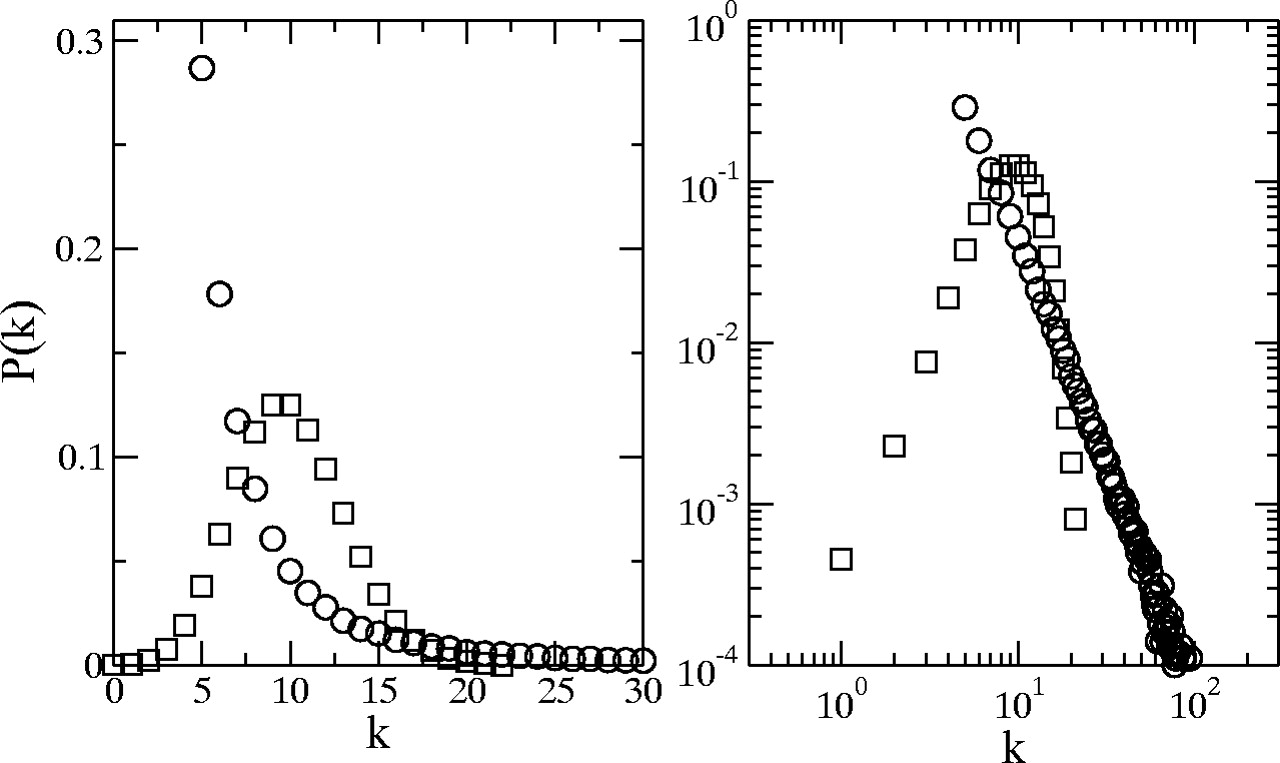
\includegraphics[scale = 0.2]{img/pois.jpeg}
  \caption{Confronto tra la \textit{distribuzione di Poisson}, rappresentata dai
    quadrati, e la \textit{power-law}, rappresentata coi cerchi, prima in scala
    normale e poi in scala logaritmica.}
  \label{fig:pois}
\end{figure}
\begin{figure}
  \centering
  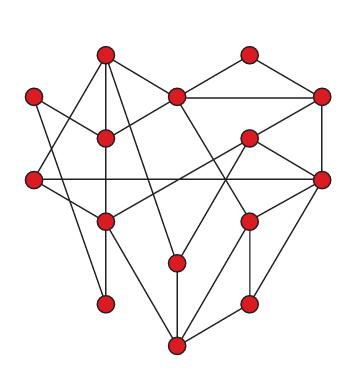
\includegraphics[scale = 2.25]{img/rnet1.jpg}\\
  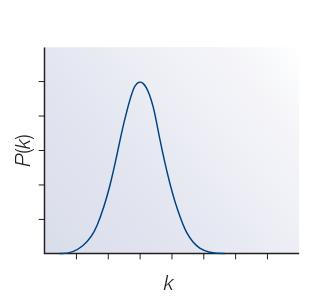
\includegraphics[scale = 1.75]{img/rnet2.jpg}
  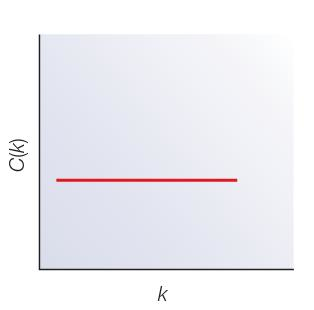
\includegraphics[scale = 1.75]{img/rnet3.jpg}
  \caption{Esempio di \textit{random network} con i grafici di $P(k)$ e $C(k)$.}
  \label{fig:rnet}
\end{figure}
\newpage
\subsection{Scale-Free Networks}
Si hanno poi le \textbf{scale-free network}, dette anche \textbf{Barabási-Albert
  model}, dal nome di coloro che le formalizzarono nel 1999.\\
Si hanno quindi le seguenti caratteristiche principali per una
\textit{scale-free network}:
\begin{itemize}
  \item la rete è \textbf{non omogenea}, da qui il nome scale-free. Si hanno
  quindi pochi nodi fortemente connessi, gli \textbf{hub}, e tanti nodi con
  pochissimi archi incidenti
  \item la \textit{degree distribution} segue la \textbf{power-law}, come
  visibile in figura \ref{fig:pois}\footnote{Réka Albert; Scale-free 
    networks in cell biology. J Cell Sci 1 November 2005; 118 (21):
    4947–4957. doi: https://doi.org/10.1242/jcs.02714}, avendo che: 
  \[P(k)=k^{-\gamma},\,\,\gamma\in\mathbb{R}\]
  dove si ha la \textit{ultra small world property} per $2<\gamma<3$, anche se
  in realtà dei valori di $\gamma$ che eccedono questo range comportano altre
  tipologie di rete
  \item non si ha \textbf{modularità intrinseca}, non avendo quindi moduli e
  avendo che$ C(k)$ è indipendente dal valore di $k$. Si hanno quindi pochi
  cluster 
\end{itemize}
\textbf{QUI MANCA UNA SLIDE FATTA A LEZIONE MA NON PRESENTE NEL PDF.}\\
Questa tipologia di rete è solitamente quella più usata in ambito
biologico, infatti possiamo ad esempio pensare ad una proteina come
\textit{p53}, tra le principali responsabili dell'\textit{apoptosi}, che in una
rete sarà sicuramente un \textit{hub}. Altri esempi possono essere le molecole
di \textit{ATP}, \textit{ADP} etc$\ldots$. Alcuni esempi sono (\textit{alcune
  immagine relative sono presenti sulle slide}): 
\begin{itemize}
  \item \textit{rete PPI per il lievito}
  \item \textit{rete di proteine per c. elegans, un eucariote}
  \item \textit{reti metaboliche per a. fulgidus, un archaea, e. coli, un
    batterio, c. elegans etc$\ldots$}, dove le reti sono modellate da grafi
  orientati e si ha che sia la \textit{indegree distribution} che la
  \textit{outdegree distribution} seguono la \textit{power-law}
\end{itemize}
Ma si hanno anche esempi non biologici come:
\begin{itemize}
  \item \textit{world wide web}
  \item \textit{connessioni tra gli aeroporti mondiali}
\end{itemize}
Interessante è cercare di capire perché i sistemi biologici tendono a comportare
\textit{scale-free network}. Si suppone infatti che tale comportamento abbia
due cause principali:
\begin{enumerate}
  \item la \textbf{crescita (\textit{growth})}
  \item il cosiddetto \textbf{attaccamento preferenziale (\textit{preferential
      attachment})} 
\end{enumerate}
Infatti questi due processi generano \textit{hub} tramite il processo detto
\textit{``rich-gets-richer''} per il quale nuovi nodi tendono a collegarsi a
nodi con un grado alto, facendo sì che i nodi con alto grado siano destinati ad
avere sempre più nodi incidenti, aumentandone ancora il grado e aumentando la
possibilità che nuovi nodi vengano attaccati a loro. Si ha inoltre che è molto
probabile che i primi nodi della rete siano quelli destinati ad avere un grado
alto che cresce all'aggiunta di nuovi nodi (cosa che porta ad avere reti
dominate da \textit{hub}). Questo comportamento è anche alla base
dell'\textit{algoritmo di PageRank}. \\
Quindi in generale si hanno varie ipotesi possibili:
\begin{itemize}
  \item l'\textit{evoluzione}
  \item \textit{ottimizzazione energetica}
  \item maggior \textit{robustezza} (concetto che si introdurrà a breve) nei con
  fronti delle perturbazioni
\end{itemize}
Un'altra teoria molto accreditata è quella, parlando di \textit{reti PPI},
rileva le origini di tali reti nella \textbf{duplicazione genica}, spiegata
visivamente in figura \ref{fig:dup}\footnote{Barabási, AL., Oltvai, Z. Network
  biology: understanding the cell's functional organization. Nat Rev Genet 5,
  101–113 (2004). https://doi.org/10.1038/nrg1272}. Quando le 
cellule si dividono, uno o più geni potrebbero essere copiati due volte nel
genoma della prole e ciò induce la crescita nella \textit{rete PPI} poiché
esiste un gene in più che codifica per una nuova proteina, avendo letteralmente
un nodo in più uguale ad un altro. La nuova proteina ha la stessa struttura
della vecchia, quindi entrambe interagiscono con le stesse proteine e le
proteine che hanno interagito con la proteina duplicata originale acquisiranno
ciascuna una nuova interazione con la nuova proteina. Inoltre le proteine con un
gran numero di interazioni tendono a ottenere collegamenti più spesso, poiché è
più probabile che interagiscano con la proteina che è stata
duplicata. Si creano così \textit{hub} e \textit{scale-free network}. Ovviamente
poi, nella realtà, tali proteine duplicate è difficile che 
restino esattamente uguali e in ogni caso non è un discorso semplice pensare di
rimuovere a priori tali nodi dalla rete.\\
\begin{figure}
  \centering
  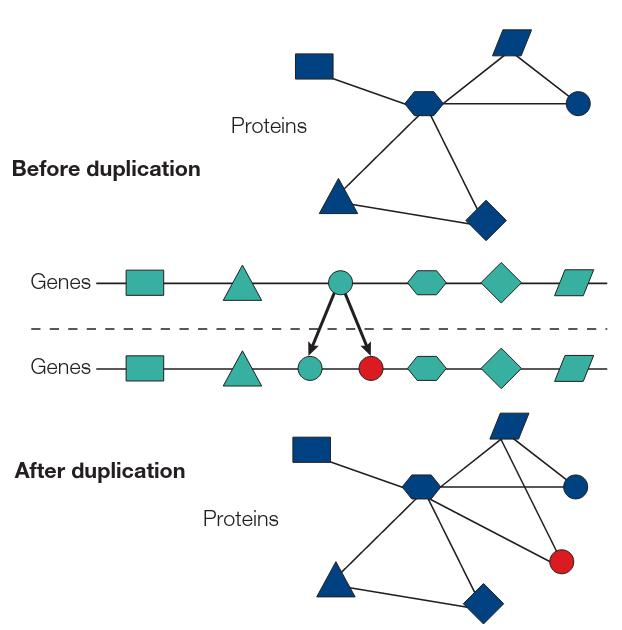
\includegraphics[scale = 1.5]{img/dup.jpg}
  \caption{Rappresentazione grafica dell'ipotetico processo di
    \textit{duplicazione genica}, che produce i due nodi rappresentati da
    cerchi, che porterebbe a \textit{scale-free network}.}  
  \label{fig:dup}
\end{figure}
Tali modelli trovano molto spazio anche fuori dal mondo biologico, basti
pensare a reti per modellare materiali etc$\ldots$\\
Un esempio di questa tipologia di rete è visibile in figura
\ref{fig:sfnet}\footnote{Barabási, AL., Oltvai, Z. Network biology: understanding
  the cell's functional organization. Nat Rev Genet 5, 101–113
  (2004). https://doi.org/10.1038/nrg1272}.
\begin{figure}
  \centering
  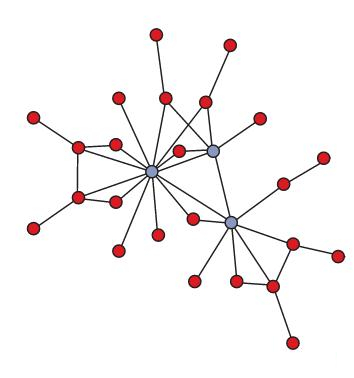
\includegraphics[scale = 2.25]{img/sfnet1.jpg}\\
  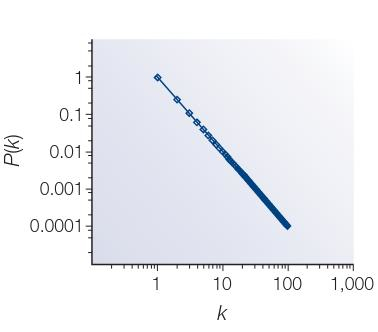
\includegraphics[scale = 1.75]{img/sfnet2.jpg}
  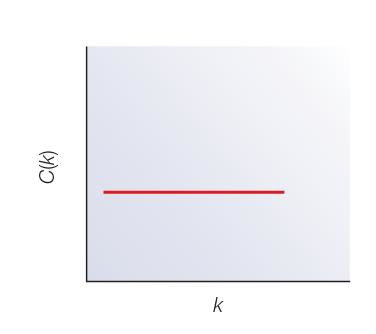
\includegraphics[scale = 1.75]{img/sfnet3.jpg}
  \caption{Esempio di \textit{scale-free network} con i grafici di $P(k)$ e
    $C(k)$. Gli \textit{hub} sono colorati in grigio.} 
  \label{fig:sfnet}
\end{figure}
\subsubsection{Robustezza Topologica}
Un altro discorso interessante da introdurre in questo contesto è quello della
``resistenza'' da parte delle \textit{scale-free} network alle
\textit{perturbazioni}. Si parla quindi di \textbf{robustezza topologica} delle
reti. 
\begin{definizione}
  Si definisce \textbf{robustezza} come l'abilità del sistema di rispondere a
  cambiamenti nelle condizioni esterne o nell'organizzazione interna, mantenendo
  un comportamento ``normale''.
\end{definizione}
Una formalizzazione matematica di un ``punteggio'' relativo alla robustezza non
è discorso banale e nemmeno unico. Si possono avere varie strategie basate sul
numero di \textit{hub}, sui pesi degli archi, sulle caratteristiche globali
della rete etc$\ldots$\\
Ci si chiede quindi:
\begin{itemize}
  \item cosa succede se si disabilita/elimina un numero sostanziale di nodi in
  una rete? 
  \item cosa succede se si verifica un errore accidentale?
  \item cosa succede se si rimuovono deliberatamente nodi specifici nella rete? 
\end{itemize}
Parlando di rimozione di nodi potrei avere infatti due casi:
\begin{enumerate}
  \item un \textbf{random attack}, dove letteralmente il nodo da eliminare è uno
  casuale e, avendo molti più nodi con basso grado che \textit{hub} (che sono
  pochissimi), si ha che la rete ``collassa'' ad un grafo sconnesso molto
  lentamente in quanto gli \textit{hub} impiegano diverse rimozioni di nodi a
  sparire 
  \item un \textbf{deliberate attack} sugli \textit{hub}, dove appunto si mira
  ad eliminare specificamente i nodi \textit{hub}. In questo caso la rete
  ``collassa'' ad un grafo sconnesso molto in fretta
\end{enumerate}
Le chance di poter studiare \textit{proprietà emergenti} da una rete è
direttamente correlata alla ``resistenza'' ai vari tipi di attacchi anche se
bisogna ricordare che non sempre avere \textit{hub} è a priori la situazione
migliore per uno studio.
\subsection{Hierarchical Networks}
Vediamo infine l'ultima tipologia di rete tratta in questo corso, le
\textbf{hierarchical networks}. Tali reti hanno comunque poco spazio nella
\textit{systems biology}.\\
Si hanno quindi le seguenti caratteristiche principali:
\begin{itemize}
  \item si ha la \textit{coesistenza} di \textbf{modularità}, \textbf{clustering
    locale} e \textbf{topologia scale-free}. Si hanno quindi cluster, poco
  collegati tra loro, con all'interno \textit{modules}
  \item la \textit{degree distribution} segue la \textbf{power-law}, come
  visibile in figura \ref{fig:pois}\footnote{Réka Albert; Scale-free 
    networks in cell biology. J Cell Sci 1 November 2005; 118 (21):
    4947–4957. doi: https://doi.org/10.1242/jcs.02714}
  \item si ha \textbf{modularità intrinseca}, avendo che $C(k)$ è proporzionale
  a $\frac{1}{k}$
\end{itemize}
Prove crescenti suggeriscono che le reti biologiche contengono piccoli
sottografi conservati dai processi evolutivi che hanno una struttura ben
definita. Possiamo quindi caratterizzarli, anche se è già stato fatto, in modo
descrittivo in quanto non esiste una vera e propria formalizzazione matematica
di essi: 
\begin{itemize}
  \item i \textbf{module}, ovvero un gruppo di nodi collegati fisicamente o
  funzionalmente che lavorano insieme per ottenere una specifica funzione
  cellulare, come ad esempio la trasduzione del segnale di una determinata
  molecola 
  \item i \textbf{motif}, ovvero sottografi che si verificano significativamente
  più frequentemente nella rete data di quanto si otterrebbe con una
  \textit{random network}
\end{itemize}
Questi due tipi di sottografo sono essenziali negli studi in \textit{systems
  biology} tramite reti ma la loro identificazione è un problema
computazionalmente complesso, oltre ad essere, come detto, non ben definito. \\
Parlando di \textit{motif} se ne possono identificare varie tipologie, come
quelle proposte da Albert\footnote{Réka Albert; Scale-free networks in cell
  biology. J Cell Sci 1 November 2005; 118 (21): 4947–4957. doi:
  https://doi.org/10.1242/jcs.02714}:
\begin{itemize}
  \item \textbf{transcriptional feed-forward loop}, ad esempio:
  \begin{figure}[H]
    \centering
    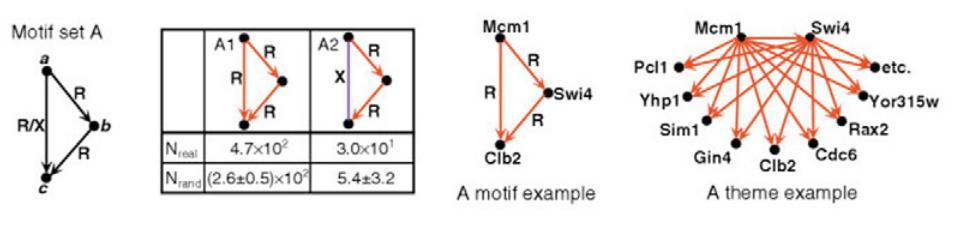
\includegraphics[width = \textwidth]{img/mot1.jpg}
  \end{figure}
  dove con $R$ si identificano gli archi per le regolazioni trascrizionali e con
  $X$ le \textit{espressioni correlate}
  \item \textbf{transcriptional co-regulation}, ad esempio:
  \begin{figure}[H]
    \centering
    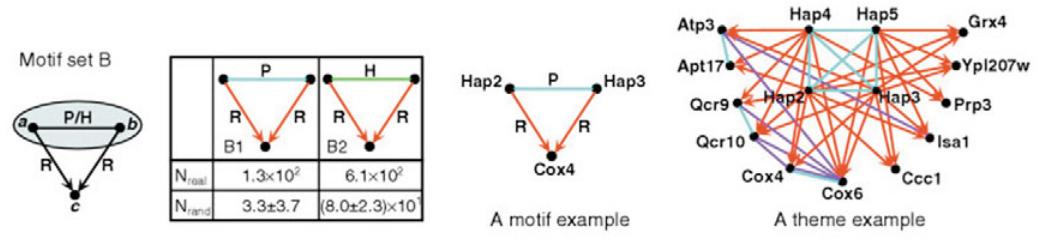
\includegraphics[width = \textwidth]{img/mot2.jpg}
  \end{figure}
  dove con $R$ si identificano gli archi per le \textit{regolazioni
    trascrizionali}, con 
  $P$ le \textit{interazioni proteiche} e con $H$ l'\textit{omologia tra
    sequenze} 
  \item \textbf{co-regulation of members of a protein complex}, ad esempio:
  \begin{figure}[H]
    \centering
    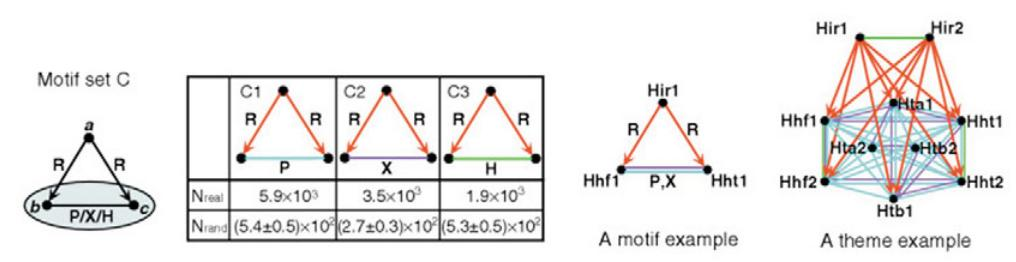
\includegraphics[width = \textwidth]{img/mot3.jpg}
  \end{figure}
  dove con $R$ si identificano gli archi per le \textit{regolazioni
    trascrizionali}, con 
  $P$ le \textit{interazioni proteiche}, con $H$ l'\textit{omologia tra
    sequenze} e con
  $X$ le \textit{espressioni correlate}
  \item \textbf{co-expressed protein cliques}, ad esempio:
  \begin{figure}[H]
    \centering
    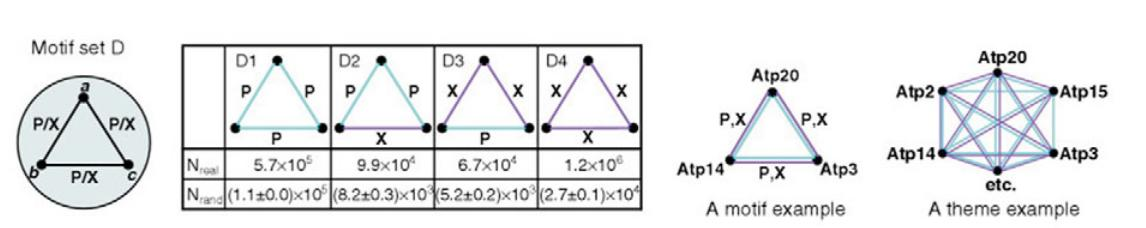
\includegraphics[width = \textwidth]{img/mot4.jpg}
  \end{figure}
  dove $P$ le \textit{interazioni proteiche} con
  $X$ le \textit{espressioni correlate}
\end{itemize}
Un esempio di questa tipologia di rete è visibile in figura
\ref{fig:sfnet}\footnote{Barabási, AL., Oltvai, Z. Network biology: understanding
  the cell's functional organization. Nat Rev Genet 5, 101–113
  (2004). https://doi.org/10.1038/nrg1272}.
\begin{figure}
  \centering
  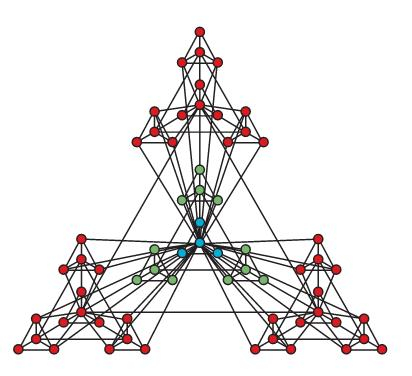
\includegraphics[scale = 2.25]{img/hnet1.jpg}\\
  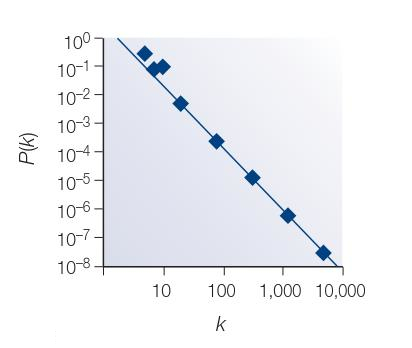
\includegraphics[scale = 1.75]{img/hnet2.jpg}
  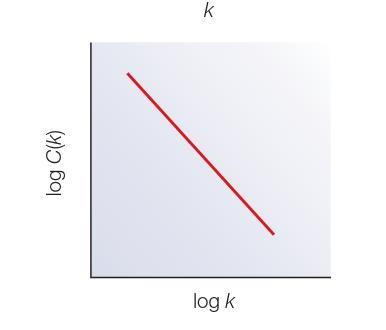
\includegraphics[scale = 1.75]{img/hnet3.jpg}
  \caption{Esempio di \textit{hierarchical network} con i grafici di $P(k)$ e
    $C(k)$. Gli \textit{hub} sono colorati in grigio.} 
  \label{fig:sfnet}
\end{figure}
\textbf{Un testo online interessante sul tema delle reti si trova al link:\\}
\begin{center}
  \url{http://networksciencebook.com}
\end{center}
\section{Software}
Per analizzare reti, biologiche ma anche non biologiche (si passa anche a studi
di scienze sociali e reti complesse generiche), uno dei tool standard
in uso è \textbf{Cytoscape}\footnote{Cline, Melissa S et al. “Integration of
  biological networks and gene expression data using Cytoscape.” Nature
  protocols vol. 2,10 (2007): 2366-82. doi:10.1038/nprot.2007.324}, disponibile
gratuitamente a 
\url{http://www.cytoscape.org/}.\\
Citando direttamente:
\begin{center}
  \textit{``Cytoscape is an open source software platform for visualizing
    molecular 
    interaction networks and biological pathways and integrating these networks
    with annotations, gene expression profiles and other state data.''\\
    ...\\
    ``Although Cytoscape was originally designed for biological research, now it
    is a 
    general platform for complex network analysis and visualization.''\\
    ...\\
    ``Cytoscape core distribution provides a basic set of features for data
    integration, 
    analysis, and visualization. Additional features are available as Apps
    (formerly called 
    Plugins). Apps are available for network and molecular profiling analyses,
    new layouts, additional file format support, scripting, and connection with
    databases.''  } 
\end{center}
Come scritto si hanno a disposizione una vasta serie di plugins, detti
\textit{apps} e ben introdotti dal paper di Saito et al.\footnote{Saito R, Smoot
ME, Ono K, et al. A travel guide to Cytoscape plugins. Nat
Methods. 2012;9(11):1069-1076. doi:10.1038/nmeth.2212}, che aggiungono
moltissime funzionalità, tra cui, ad esempio, 
collegare una rete ad un database esterno per fare \textit{gene enrichment}. 
\chapter{Logic-Based Modelling}
Si introducono ora i \textbf{modelli logic-based}.\\
Ricordiamo che tali modelli, come visibile in figura \ref{fig:appro}:
\begin{itemize}
  \item sono sistemi meno \textit{large-scale} di quanto lo fossero i
  \textit{modelli interaction-based}
  \item presentano tendenzialmente un basso costo computazionale
  \item presentano un livello di dettaglio, per quanto ambiguo nello schema,
  variabile
  \item presentano alcune difficoltà nella misurazione dei dati
\end{itemize}
Il tutto comporta una miglior capacità predittiva rispetto ai \textit{modelli
  interaction-based} e, grazie all'uso di vari tipi di logiche, può portare
anche a ottenere modelli molto più predittivi.\\
Un'altra differenza sostanziale rispetto ai \textit{modelli interaction-based} è
che si può iniziare a parlare di \textit{simulazioni}, superando il ``limite''
delle sole analisi. In questo caso i modelli più semplici si basano sulla
\textit{logica booleana} e, come si vedrà, se simulazioni e le analisi
consistono nel determinare:
\begin{itemize}
  \item \textbf{cicli}, ovvero sequenze ripetute di stati di sistema
  \item \textbf{attrattori}, ovvero stati finali raggiungibili da un qualsiasi
  stato iniziale
  \item \textbf{bacini di attrazione}, percorsi di stati intermedi che iniziano
  da uno stato iniziale e terminano in un attrattore
\end{itemize}
Con l'aggiunta della \textbf{logica fuzzy}, più complessa di quella booleana, si
può anche derivare il \textit{comportamento dinamico} del sistema, ad esempio
derivando la variazione temporale del valore di ogni componente in uno o più
stati, magari dopo una certa \textit{perturbazione}. Si parla quindi di
\textbf{modelli qualitativi} e 
\textbf{dinamici}. L'informazione \textit{quantitativa} è ridotta al minimo, non
avendo la rappresentazione di vere e proprie interazioni/proprietà chimiche e
fisiche 
come, ad esempio, la rappresentazione di \textit{kinetic-rate} etc$\ldots$\\ 
Come detto si hanno sia \textit{sistemi small-scale} che \textit{sistemi
  large-scale}, anche se comunque di dimensioni ridotte rispetto ai
\textit{modelli interaction-based}, e ad esempio sono usati per:
\begin{itemize}
  \item \textbf{reti di regolazione gene-gene}
  \item \textbf{pathway per il segnale di trasduzione}
  \item \textbf{differenziazione cellulare}, soprattutto grazie allo studio
  degli \textit{attrattori}
  \item \textbf{pathway per la morte programmata cellulare}
\end{itemize}
Tecnologie sperimentali di natura qualitativa (ad esempio \textit{targeting
  genico} e \textit{screening fenotipici}) hanno portato allo sviluppo di metodi
computazionali per modellare e analizzare reti regolatorie geniche sulla base di
regole logiche. L'architettura di tali modelli, per semplificare, consiste in
due ``aspetti'' principali:
\begin{enumerate}
  \item la \textbf{struttura della rete}, modellata tramite \textit{grafi
    diretti}, dove con la direzione si specificano principalmente, ma non solo,
  fenomeni di regolazione
  \item le \textbf{dinamiche della rete}, modellati tramite stati logic-based
  mutevoli e funzioni di update degli stati stessi, che garantiscono
  un'evoluzione nel tempo
\end{enumerate}
L'idea generale è quindi quella di partire da uno \textbf{stato iniziale} per
poi assegnare un nuovo valore ad ogni variabile del modello, quindi ad ogni nodo
della rete, tramite l'uso di \textit{funzioni logiche} che combinano i valori
delle variabili dello stato corrente per produrre il nuovo stato.\\
Interessante è elencare fin da subito alcuni \textbf{pro} di questo approccio
modellistico:
\begin{itemize}
  \item i \textit{modelli logic-based} sono \textbf{versatili}, in quanto una
  variabile può praticamente rappresentare qualsiasi cosa, come ad esempio un
  gene, un'attività genica, la presenza di una proteina, un fenotipo, lo stato
  di una cellula etc$\ldots$ Inoltre si possono mischiare componenti eterogenee
  in modo abbastanza semplice, a differenza di quanto accadeva coi
  \textit{modelli interaction-based}, dove era molto più complesso fare ciò
  \item i \textit{modelli logic-based} sono \textbf{flessibili}, in quanto lo
  stato di un dato componente cellulare può essere rappresentato da una o più
  variabili, con diversi insiemi di valori. Quindi una certa componente può
  avere funzioni diverse a seconda dello stato del sistema e questo risolve
  quanto visto nel caso dei \textit{modelli interaction-based} in merito ai
  nodi ripetuti nella rete, avendo che in questo caso i due o più nodi sono
  ben distinti, magari avendo un nodo per una certa proteina e un altro per la
  stessa proteina ma fosforilata (si ricorda che la \textit{fosforilazione} è
  una reazione chimica, fondamentale in biochimica,  che consiste
  nell'addizione di un gruppo fosfato, $PO_4^{3-}$, ad una proteina o ad
  un'altra molecola e si ricorda che gli enzimi che solitamente catalizzano le
  fosforilazioni sono le chinasi)   
  \item gli effetti delle \textit{perturbazioni}, come \textit{inibizioni} o
  \textit{mutazioni}, possono essere ``testati'' in modo molto facile e diretto
\end{itemize}
Si hanno però anche vari \textbf{contro}, che principalmente si riconducono al
fatto che non sono modelli meccanicistici. Infatti, per quanto si abbia alla
base un \textit{grafo diretto}, non è possibile inferire la proprietà
meccanicistica che si ha dietro la regolazione positiva/negativa, o altro, che
viene rappresentata mediante l'arco diretto. Ipotizziamo anche solo di avere due
nodi $A$ e $B$, con $A$ che regola $B$:
\begin{center}
  \begin{tikzpicture}[shorten >=1pt,node distance=2cm,on grid,auto]
    \node[state] (q_0) {$A$};
    \node[state] (q_1) [right=of q_0] {$B$};
    \path[->]
    (q_0) edge  node {} (q_1);
  \end{tikzpicture}
\end{center}
Potremmo dire che ``l'attività di $A$ stimola l'attività di $B$'' e si può
modellare una regolazione positiva o negativa ma non
potremo mai caratterizzare nel dettaglio il meccanismo stesso, che potrebbe
essere, ad esempio: 
\begin{itemize}
  \item l'attivazione della produzione di $B$
  \item l'inibizione della degradazione di $B$
  \item la stabilizzazione dell'\textit{high-activity state} di $B$
  \item $\ldots$
\end{itemize}
Posso solo sapere che c'è uno stimolo, avendo infatti perdita d'informazione che
impedisce l'inferenza dei meccanicismi. \\
Nei paragrafi precedenti si sono nominate spesso le
\textit{variabili}. Approfondendo il discorso si ha che in modello matematico
esse possono essere:
\begin{itemize}
  \item \textbf{valori booleani}, ovvero valori binari come 0/1,
  presente/assente, attivo/inattivo etc$\ldots$
  \item \textbf{valori multi-stato}, sia \textbf{linguistici} che
  \textbf{numerici}, come ad esempio nullo/basso/medio/alto, 0/1/2/3 etc$\ldots$
  \item \textbf{valori numerici interi o reali}, usati ad esempio per
  rappresentare la concentrazione o il numero di molecole
\end{itemize}
Le prime due categorie sono quindi sono a \textit{valori discreti} mentre la
terza è a \textit{valori continui}. Una categorizzazione più precisa, parlando
di \textit{modelli-logic based} si può osservare in figura
\ref{fig:log}\footnote{Morris MK, Saez-Rodriguez J, Sorger PK, Lauffenburger
  DA. Logic-based models for the analysis of cell signaling
  networks. Biochemistry. 2010;49(15):3216-3224. doi:10.1021/bi902202q}. \\ 
È stato anche citato il cosiddetto \textit{stato iniziale del sistema}, ovvero
la \textit{condizione iniziale} del modello, che prevede l'assegnamento di un
valore, all'inizio della simulazione, ad ogni variabile del sistema. La
\textit{condizione iniziale} influisce ovviamente i risultati stessi della
simulazione, determinando come evolve il sistema nel tempo, soprattutto se si ha
una simulazione deterministica.
\begin{figure}
  \centering
  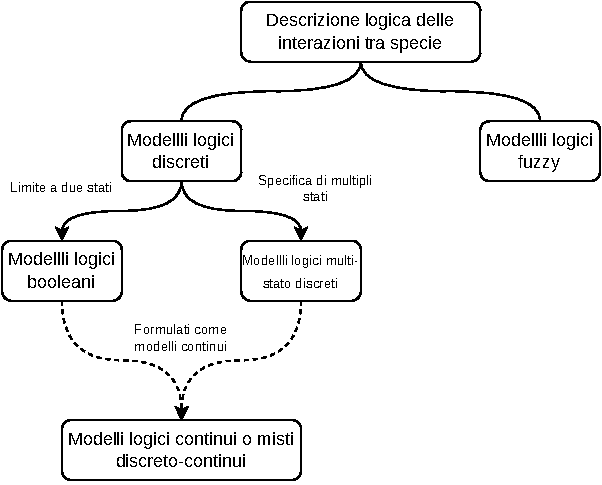
\includegraphics[scale = 1]{img/log.pdf}
  \caption{Schema riassuntivo dell'uso delle variabili in modelli
    \textit{logic-based}.}
  \label{fig:log}
\end{figure}
\newpage
\noindent
Ovviamente la scelta tra discreto e continuo comporta delle
conseguenze. Prendiamo ad esempio la seguente situazione:
\begin{center}
  \begin{tikzpicture}[shorten >=1pt,node distance=2cm,on grid,auto]
    \node[state] (q_0) {$Y$};
    \node[state] (q_1) [right=of q_0] {$X$};
    \path[->]
    (q_0) edge  node {} (q_1);
  \end{tikzpicture}
\end{center}
e il seguente grafico\footnote{Albert, Reka, and
  Juilee Thakar. "Boolean modeling: a logic‐based dynamic approach for
  understanding signaling and regulatory networks and for making useful
  predictions." Wiley Interdisciplinary Reviews: Systems Biology and Medicine
  6.5 (2014): 353-369.}, che descrive la regolazione positiva di $Y$ su $X$: 
\begin{figure}[H]
  \centering
  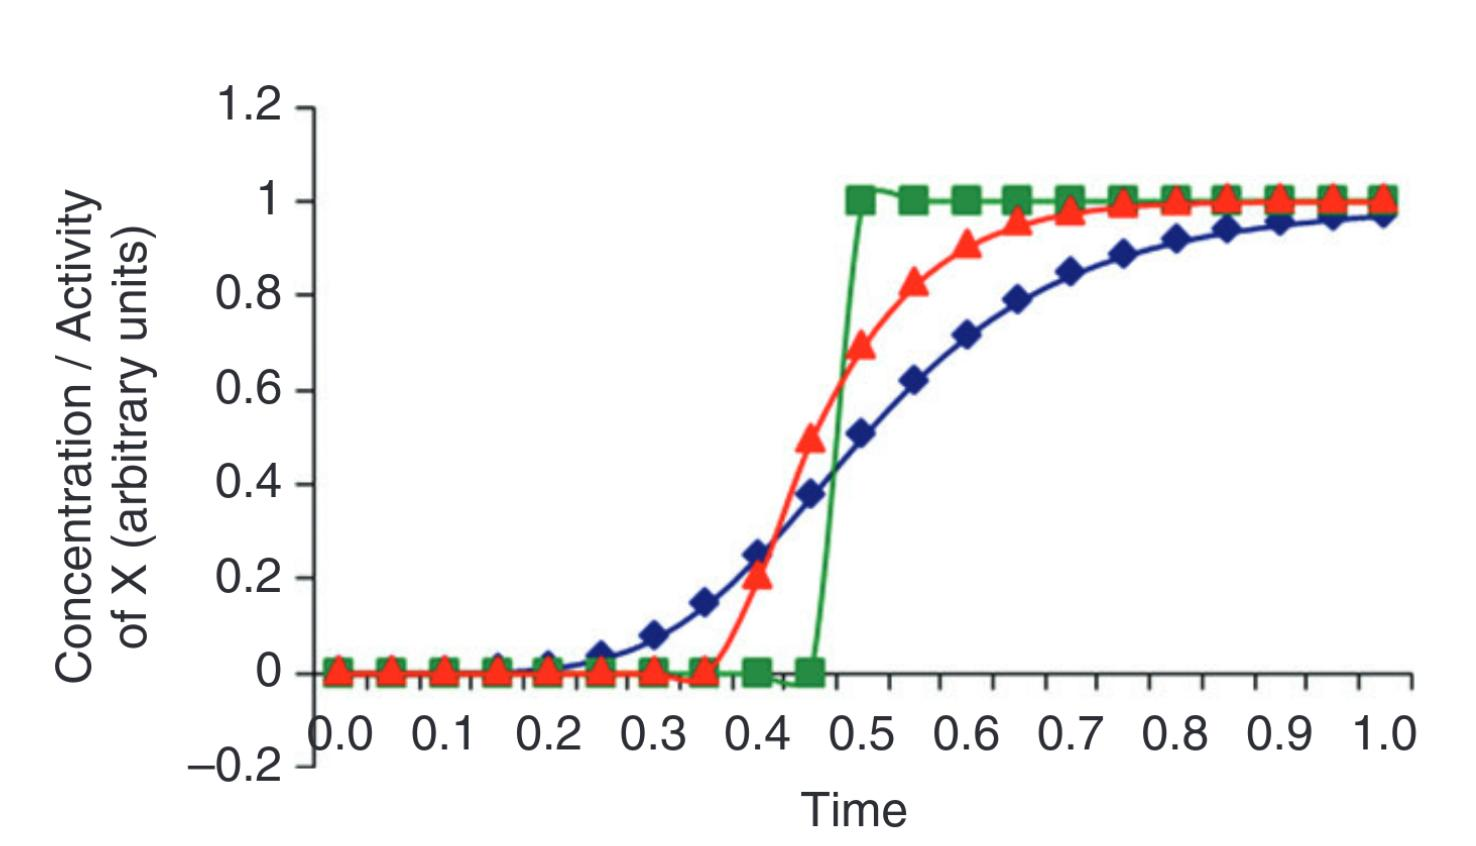
\includegraphics[scale = 0.2]{img/boolf.jpg}
\end{figure}
Nel grafico si hanno:
\begin{itemize}
  \item sull'asse delle ascisse il tempo
  \item sull'asse delle ordinate la concentrazione del nodo $X$ (si assume che
  la concentrazione/attività del nodo $Y$ cresca linearmente)
  \item la funzione booleana in verde
  \item due funzioni continue in rosso e blu che rappresentano il ``caso reale''
\end{itemize}
Si nota come il ``cambio'' per la funzione booleana sia ``secco'', prima 0 e poi
1, un certo momento temporale. Questa eccessiva semplificazione non sempre è
accettabile per descrivere casi reali ma ci sono situazioni in cui è comunque
accettabile. Potrei avere anche altre funzioni, magari multi-stato, come quelle
in figura \ref{fig:funbool}\footnote{Morris MK, Saez-Rodriguez J, Sorger PK,
  Lauffenburger DA. Logic-based models for the analysis of cell signaling 
  networks. Biochemistry. 2010;49(15):3216-3224. doi:10.1021/bi902202q}
\begin{figure}
  \centering
  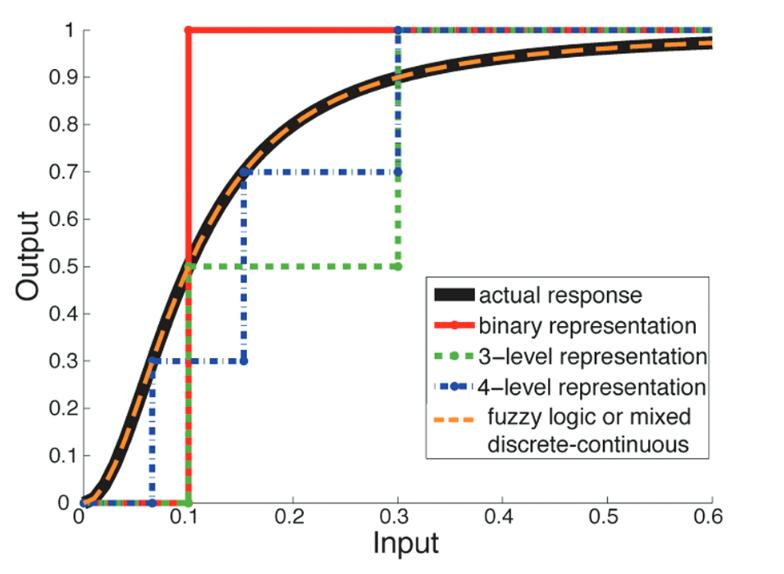
\includegraphics[scale = 0.35]{img/funbool.jpg}
  \caption{Esempio di approssimazioni di un certo andamento, partendo
    dall'approssimazione  booleana a
    quella nel caso continuo, che rappresenta correttamente la relazione
    a sigmoide tra i livelli di input e output ad esempio nel casi dell'azione
    della chinasi su un substrato, passando per diverse approssimazioni
    multi-strato.}  
  \label{fig:funbool}
\end{figure}
Si può quindi rilevare un ulteriore \textbf{contro} che si può avere in
\textit{sistemi logic-based} in quanto quando un nodo è ``off'', ad esempio, non
significa esattamente che la molecola ha zero concentrazione in quel momento nel
sistema. Si sottintende una \textit{soglia implicita} che stabilisce ``on''  e
``off'', quindi è ``off'' sse la molecola non è presente in modo
sufficiente al punto da permettere cambiamenti nelle molecole regolate da
essa. Quando supera quella soglie diventa ``on'' (ad esempio si può pensare di
avere $0\leq x\leq 1$ e che fino a $x=0.8$ si ha lo stato ``off'' e con $x>0.8$
lo stato ``on''). Si ha quindi solo
un'approssimazione qualitativa della regolazione molecolare anche se bisogna
notare che noti che molti dati sperimentali disponibili sulle regolazioni
molecolari sono di natura qualitativa. \\
Si possono, come anticipato, fare delle \textit{simulazioni} e l'aggiornamento
degli stati può essere determinato in vari modi, tramite diverse concezioni del \textit{tempo}:
\begin{itemize}
  \item tramite \textbf{iterazioni} che non rappresentano necessariamente una
  durata temporale fisica specifica, infatti un ``passo temporale'', un
  \textit{time step} può rappresentare una durata diversa per iterazioni diverse
  (magari in un caso è un evento che avviene in un secondo e in un altro che
  avviene in un'ora ma entrambi sono un singolo \textit{time step} di ugual
  durata). Si hanno inoltro due ulteriori sotto casistiche:
  \begin{enumerate}
    \item la \textbf{modalità di aggiornamento sincrona}, dove il valore di
    tutte le variabili viene ricalcolato dopo ogni singola
    iterazione. \textit{Questa sarà la modalità che verrà approfondita nel
      corso}  
    \item la \textbf{modalità di aggiornamento asincrona}, dove le variabili
    subiscono transizioni una alla volta e le variabili da aggiornare vengono
    scelte in modo tendenzialmente causale
  \end{enumerate}
  \item tramite \textbf{step discreti}, che quindi hanno una specifica durata
  eventualmente diversa l'uno dagli altri, dopo i quali avvengono gli
  aggiornamenti delle variabili
  \item \textbf{tempo continuo}, dove si simula (eventualmente su una scala
  diversa) il trascorrere reale del tempo
\end{itemize}
Un'altra problematica che si presenta dopo aver capito come viene aggiornato lo
stato del sistema in un \textit{modello logic-based} è quello che il numero di
stati cresce in modo esponenziale rispetto al numero di variabili, quindi al
numero di nodi $|V|$. Questo aspetto rende complicata anche la validazione dei
modelli, validazioni che solitamente vengono fatte in modo probabilistico
(\textit{aspetto non ben chiarito a lezione ma magari si vedrà più avanti nel
  corso}). Inoltre, avendo nei \textit{modelli logic-based} solitamente l'uso di
iterazioni per descrivere l'evoluzione temporale si ha difficoltà a tracciare
processi lenti/veloci o anche \textit{ritardi}, spesso frequenti nei sistemi
biologici.\\
Come detto ad ogni iterazione si ha una \textbf{transizione di stati}, quindi
l'\textit{aggiornamento degli stati}, che avviene dopo la computazione di un
insieme di \textit{funzioni logiche} assegnate ad ogni variabile del modello,
quindi ad ogni nodo del grafo nel nostro caso. Si hanno quindi:
\begin{itemize}
  \item gli \textbf{operatori booleani}, nel caso specifico un sottoinsieme
  degli stessi composto da $\land$ (l'\textit{and logico}), $\lor$ (l'\textit{or
    logico}) e il $\neg$ (il \textit{not logico})
  \item le \textbf{espressioni booleane} ottenute tramite gli \textit{operatori
    booleani} 
\end{itemize}
Dopo che si è definita la logica di un modello e si è costruito il modello
stesso si possono produrre le cosiddette \textbf{traiettorie}, dette anche
\textbf{pseudo time-courses}, quindi sequenze di stati raggiungibili
consecutivamente ognuno a partire dal precedente, e studiare eventuali
\textit{attrattori} etc$\ldots$ Ovviamente, poiché il tempo non è correlato al
tempo fisiologico/reale, i modelli booleani possono fornire solo una cronologia
qualitativa delle attivazioni dei nodi.
\section{Introduzione alla Logica Booleana}
Prima di procedere occorre fare un piccolo ripasso di logica booleana, anche per
poterla collegare a situazioni biologiche.\\
Come anticipato abbiamo tre \textit{operatori logici}:
\begin{enumerate}
  \item il \textit{not}, indicato solitamente con $\neg$, è un operatore unario
  che viene rappresentato, a livello circuitale tramite:
  \begin{center}
    \begin{tikzpicture}[circuit logic US]
      \node [not gate] (and1) {};
      \draw (and1.input) -- node[at end,left]{A} ++(left:4mm);
      \draw (and1.output) -- node[at end,right]{B} ++(right:4mm);
    \end{tikzpicture}
  \end{center}
  e al quale corrisponde la seguente tabella di verità:
  \begin{table}[H]
    \small
    \centering
    \begin{tabular}{c|c}
      $A$&$B=\neg A$\\
      \hline
      0 & 1 \\
      1 & 0
    \end{tabular}
  \end{table}
  \item l'\textit{and}, indicato solitamente con $\land$, è un operatore binario
  che viene rappresentato, a livello circuitale tramite:
  \begin{center}
    \begin{tikzpicture}[circuit logic US]
      \node [and gate, inputs=nnn] (and1) {};
      \draw (and1.input 1) -- node[at end,left]{\footnotesize{A}} ++(left:4mm);
      \draw (and1.input 3) -- node[at end,left]{\footnotesize{B}} ++(left:4mm);
      \draw (and1.output) -- node[at end,right]{C} ++(right:4mm);
    \end{tikzpicture}
  \end{center}
  e al quale corrisponde la seguente tabella di verità:
  \begin{table}[H]
    \small
    \centering
    \begin{tabular}{c|c|c}
      $A$&$B$&$C=A\land B$\\
      \hline
      0 & 0 & 0 \\
      0 & 1 & 0\\
      1 & 0 & 0\\
      1 & 1 & 1 
    \end{tabular}
  \end{table}
  \item l'\textit{or}, indicato solitamente con $\lor$, è un operatore binario
  che viene rappresentato, a livello circuitale tramite:
  \begin{center}
    \begin{tikzpicture}[circuit logic US]
      \node [or gate, inputs=nnn] (and1) {};
      \draw (and1.input 1) -- node[at end,left]{\footnotesize{A}} ++(left:4mm);
      \draw (and1.input 3) -- node[at end,left]{\footnotesize{B}} ++(left:4mm);
      \draw (and1.output) -- node[at end,right]{C} ++(right:4mm);
    \end{tikzpicture}
  \end{center}
  e al quale corrisponde la seguente tabella di verità:
  \begin{table}[H]
    \small
    \centering
    \begin{tabular}{c|c|c}
      $A$&$B$&$C=A\lor B$\\
      \hline
      0 & 0 & 0 \\
      0 & 1 & 1\\
      1 & 0 & 1\\
      1 & 1 & 1 
    \end{tabular}
  \end{table}
\end{enumerate}
Un'\textit{espressione booleana} è appunto la combinazione degli
\textit{operatori booleani} e delle \textit{variabili booleane}. Uno dei
problemi è che, date $n$ variabili booleane (quindi $|v|=n$ nodi), si hanno
esattamente $2^n$ possibili combinazioni di valori di stato, avendo $2^n$ righe
nella tavola di verità.\\
Un esempio potrebbe essere la seguente espressione booleana:
\[C=(A\land B)\lor (\neg B)\]
alla quale corrisponde la seguente tabella di verità:
\begin{table}[H]
  \small
  \centering
  \begin{tabular}{c|c|c|c|c}
    $A$&$B$&$A\land B$ & $\neg B$ & $C$\\
    \hline
    0 & 0 & 0 & 1 & 1\\
    0 & 1 & 0 & 0 & 0\\
    1 & 0 & 0 & 1 & 1\\
    1 & 1 & 1 & 0 & 1
  \end{tabular}
\end{table}
\section{Simulazioni su Modelli Logic-Based}
Si riprende per comodità un esempio già visto nell'introduzione ai modelli per
avere un esempio di quanto detto rapportato alla regolazione
molecolare\footnote{Wynn ML, Consul N, Merajver SD, 
  Schnell S. Logic-based models in systems biology: a predictive and
  parameter-free network analysis method. Integr Biol
  (Camb). 2012;4(11):1323-1337. doi:10.1039/c2ib20193c}:
\begin{figure}[H]
  \centering
  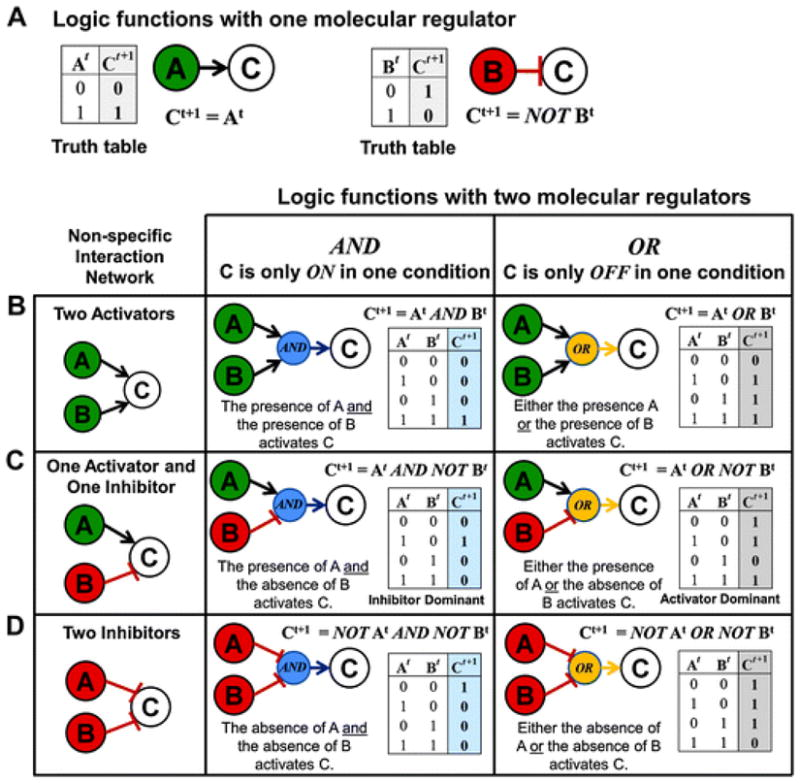
\includegraphics[scale = 0.65]{img/logicnet.jpg}
\end{figure}
In questo esempio notiamo come possiamo differenziare regolazioni positive, come
quella di $A$ su $C$, e quelle negative, come quella di $B$ su $C$, anche a
livello grafico. Notiamo anche come il formalismo sia del tipo:
\[C^{t+1}=\neg B^t\]
indicando con gli apici lo step temporale, avendo quindi specificato che lo
stato risultante in $C$ al tempo $t+1$ dipende da quello di $B$ al tempo
$t$. Ovviamente questi esempi, con le rispettive tabelle diversità, sono
minuscoli, infinitamente più piccoli rispetto a modelli logici
reali. Nell'esempio possiamo comunque vedere le varie casistiche dove $A$ attiva
$C$, facendo regolazione positiva, mentre $B$ lo inibisce, facendo regolazione
negativa, vedendo i vari risultati possibili nelle varie possibili combinazioni
di ``input''.\\
Nel dettaglio, inoltre, lo stato del sistema al tempo $t$ corrisponde ad un
vettore booleano consistente nel valore di ogni variabile booleana al tempo
$t$. Purtroppo a volte non abbiamo informazioni biologiche per assegnare la
funzione booleana al nodo e ovviamente la questione si complica all'aumentare
dei nodi regolatori, positivamente e negativamente, del nodo in
questione. Quindi alla semplicità matematica si associa in questo caso anche un
``lack'' di informazioni biologiche preliminari. \\
Si procede quindi dallo \textit{stato iniziale}, che viene definito per $t=0$, e
si calcola la traiettoria che si ha a partire da quello stato, che viene
composta quindi dall'insieme degli stati a $t=1$, $t=2$, $t=3$ etc$\ldots$ dove
il tempo è una \textbf{variabile discreta}, avendo quindi $\{t,
t+1,t+2,\ldots\}$, e dove si assume aggiornamenti in \textit{modalità sincrona}.
Fatte queste premesse è ovvio che lo stato corrente del sistema è identificato
univocamente dallo stato precedente, che a sua volta identificava univocamente
lo stato corrente come suo successore. Si ha quindi che i \textit{modelli
  logic-based booleani sincroni} sono \textbf{deterministici}, avendo che un
certo input produrrà sempre e solo lo stesso output.\\
Sfruttiamo ora un esempio per caratterizzare meglio \textit{attrattori} e
\textit{bacini di attrazione}.\\
Sia data la seguente rete:
\begin{center}
  \begin{tikzpicture}[shorten >=1pt,node distance=2cm,on grid,auto]
    \node[state] (q_0) {$A$};
    \node[state] (q_1) [below right=of q_0] {$C$};
    \node[state] (q_2) [above right=of q_1] {$B$};
    \path[->]
    (q_1) edge  node {} (q_0)
    (q_2) edge  node {} (q_1)
    (q_2) edge  node {} (q_0)
    (q_0) edge [bend left = 25] node {} (q_2);
  \end{tikzpicture}
\end{center}
\newpage
\noindent
Alla quale vengono aggiunte le seguenti funzioni booleane:
\begin{itemize}
  \item $f(A)=B\land (\neg C)$
  \item $f(B)=A$
  \item $f(C)=B$
\end{itemize}
Si ha quindi la seguente tabella di verità, che avendo $3$ variabili/nodi avrà
$2^3=8$ possibili combinazioni di stati di nodi, avendo che ogni riga della
tabella di verità rappresenta uno stato della rete:
\begin{table}[H]
  \centering
  \begin{tabular}{c|c|c||c|c|c}
    $A$&$B$&$C$&$f(A)$ & $f(B)$ & $f(C)$\\
    \hline
    0 & 0 & 0 & 0 & 0 & 0\\
    0 & 0 & 1 & 0 & 0 & 0\\
    0 & 1 & 0 & 1 & 0 & 1\\
    0 & 1 & 1 & 0 & 0 & 1\\
    1 & 0 & 0 & 0 & 1 & 0\\
    1 & 0 & 1 & 0 & 1 & 0\\
    1 & 1 & 0 & 1 & 1 & 1\\
    1 & 1 & 1 & 0 & 1 & 1\\
  \end{tabular}
\end{table}
Possiamo quindi distinguere uno \textit{stato iniziale} che comporta un
\textbf{ciclo} o un \textbf{punto fisso}. Infatti, ad esempio, se parto da
$[1,0,0]$ avrò la seguente traiettoria: 
\[[1,0,0]\Rightarrow [0,1,0]\Rightarrow [1,0,1] \Rightarrow [0,1,0]\Rightarrow
  [1,0,1]\Rightarrow\cdots\]
Avendo quindi che si ha un \textbf{ciclo} tra gli stati $[0,1,0]$ e $[1,0,1]$,
che funge da \textit{attrattore}.\\
D'altro canto se si seleziona come \textit{stato iniziale} $[1,1,0]$ avrò la
seguente traiettoria:
\[[1,1,0]\Rightarrow[1,1,1]\Rightarrow[0,1,1]\Rightarrow[0,0,1]
  \Rightarrow[0,0,0]\Rightarrow[0,0,0]\Rightarrow\ldots\]
raggiungendo quindi un \textbf{punto fisso}, un \textit{attrattore}, ovvero lo
stato $[0,0,0]$. Nel dettaglio inoltre, in questo caso semplice e fortuito, il
\textbf{bacino di attrazione} per l'attrattore $[0,0,0]$ e formato da tutte le
traiettorie che partono dagli
stati presenti nella \textit{traiettoria} che parte dallo stato $[1,1,0]$,
ovvero dagli stati dell'insieme (\textbf{capire se attrattore è nel suo stesso
  bacino di attrazione}): 
\[\{[1,1,0],\,\,[1,1,1],\,\,[0,1,1],\,\,[0,0,1],\,\,[0,0,0]\}\]
Data quindi una \textit{rete booleana} e una traiettoria sufficientemente lunga
prima o poi lo stato della rete sarà una ripetizione di una sequenza di stati
già incontrata, questo perché si ha un numero di stati totali \textbf{finito},
in quanto \textbf{discreto}.\\
Visto l'esempio possiamo raffinare quindi quanto già definito:
\begin{itemize}
  \item un \textbf{attrattore} è definito come \textbf{punto fisso
    (\textit{fixed state})} qualora si abbia che un singolo stato appare
  ripetutamente in una \textit{traiettoria}
  \item un \textbf{attrattore} è definito come \textbf{ciclo} se un insieme di
  stati appare più di una volta in una \textit{traiettoria}
\end{itemize}
Avendo quindi che un \textbf{attrattore} rappresenta uno stato dal quale non è
possibile scappare a meno che non si verifichi una \textit{perturbazione}
esterna al sistema stesso mentre un \textbf{bacino di attrazione} è l'insieme di
tutte le traiettorie che terminano in un \textit{attrattore}.
\end{document}

% LocalWords:  rewiring trascrizionali regolatorie degree distribution update
% LocalWords:  multipartiti fosforilata